\documentclass[a4paper, 11pt]{article}
\usepackage[pdftex]{graphicx}
\usepackage{fullpage}
\usepackage{mathrsfs,amsmath}
\usepackage{framed, color, fancybox}
\usepackage{todonotes}

\definecolor{shadecolor}{rgb}{0.8, 0.8, 0.2}
%define the title
\author{Seogi Kang}
\title{On recovering of distributed IP parameters in time domain electromagnetic data}

% My equations
%-----------------------------------------------------------
\renewcommand{\div}{\nabla\cdot}
\newcommand{\grad}{\vec \nabla}
\newcommand{\curl}{{\vec \nabla}\times}
\newcommand {\J}{{\vec J}}
\renewcommand{\H}{{\vec H}}
\newcommand {\E}{{\vec E}}
\newcommand{\siginf}{\sigma_\infty}
\newcommand{\dsig}{\triangle\sigma}
\newcommand{\dcurl}{{\mathbf C}}
\newcommand{\dgrad}{{\mathbf G}}
\newcommand{\Acf}{{\mathbf A_c^f}}
\newcommand{\Ace}{{\mathbf A_c^e}}
\renewcommand{\S}{{\mathbf \Sigma}}
\newcommand{\St}{{\mathbf \Sigma_\tau}}
\newcommand{\T}{{\mathbf T}}
\newcommand{\Tt}{{\mathbf T_\tau}}
\newcommand{\diag}{\mathbf{diag}}
\newcommand{\M}{{\mathbf M}}
\newcommand{\MfMui}{{\M^f_{\mu^{-1}}}}
\newcommand{\MfMuoi}{{\M^f_{\mu_0^{-1}}}}
\newcommand{\dMfMuI}{{d_m (\M^f_{\mu^{-1}})^{-1}}}
\newcommand{\dMfMuoI}{{d_m (\M^f_{\mu_0^{-1}})^{-1}}}
\newcommand{\MeSig}{{\M^e_\sigma}}
\newcommand{\MeSigInf}{{\M^e_{\sigma_\infty}}}
\newcommand{\MeSigInfEtab}{{\M^e_{\sigma_\infty \bar{\eta}}}}
\newcommand{\MeSigInfEtat}{{\M^e_{\sigma_\infty \peta}}}
\newcommand{\MedSig}{{\M^e_{\triangle\sigma}}}
\newcommand{\MeSigO}{{\M^e_{\sigma_0}}}
\newcommand{\Me}{{\M^e}}
\newcommand{\Js}{\mathbf{J}^s}
\newcommand{\Mes}[1]{{\M^e_{#1}}}
\newcommand{\Mee}{{\M^e_e}}
\newcommand{\Mej}{{\M^e_j}}
\newcommand{\BigO}[1]{\mathcal{O}\bigl(#1\bigr)}
\newcommand{\bE}{\mathbf{E}}
\newcommand{\bEp}{\mathbf{E}^p}
\newcommand{\bB}{\mathbf{B}}
\newcommand{\bBp}{\mathbf{B}^p}
\newcommand{\bEs}{\mathbf{E}^s}
\newcommand{\bBs}{\mathbf{B}^s}
\newcommand{\bH}{\mathbf{H}}
\newcommand{\B}{\vec{B}}
\newcommand{\D}{\vec{D}}
\renewcommand{\H}{\vec{H}}
\newcommand{\s}{\vec{s}}
\newcommand{\bfJ}{\bf{J}}
\newcommand{\vecm}{\vec m}
\renewcommand{\Re}{\mathsf{Re}}
\renewcommand{\Im}{\mathsf{Im}}
\renewcommand {\j}  { {\vec j} }
\newcommand {\h}  { {\vec h} }
\renewcommand {\b}  { {\vec b} }
\newcommand {\e}  { {\vec e} }
\renewcommand {\d}  { {\vec d} }
\renewcommand {\u}  { {\vec u} }

\renewcommand {\dj}  { {\mathbf{j} } }
\renewcommand {\dh}  { {\mathbf{h} } }
\newcommand {\db}  { {\mathbf{b} } }
\newcommand {\de}  { {\mathbf{e} } }

\newcommand{\vol}{\mathbf{v}}
\newcommand{\I}{\vec{I}}
\newcommand{\A}{\mathbf{A}}
\newcommand{\bI}{\mathbf{I}}
\newcommand{\bus}{\mathbf{u}^s}
\newcommand{\brhss}{\mathbf{rhs}_s}
\newcommand{\bup}{\mathbf{u}^p}
\newcommand{\brhs}{\mathbf{rhs}}
%%-------------------------------
\newcommand{\bon}{b^{on}(t)}
\newcommand{\bp}{b^{p}}
\newcommand{\dbondt}{\frac{db^{on}(t)}{dt}}
\newcommand{\dfdt}{\frac{df(t)}{dt}}
\newcommand{\dfdtdsiginf}{\frac{\partial\frac{df(t)}{dt}}{\partial\siginf}}
\newcommand{\dfdsiginf}{\frac{\partial f(t)}{\partial\siginf}}
\newcommand{\dbgdsiginf}{\frac{\partial b^{Impulse}(t)}{\partial\siginf}}
\newcommand{\digint}{\frac{2}{\pi}\int_0^{\infty}}
\newcommand{\Gbiot}{\mathbf{G}_{Biot}}
%%-------------------------------
\newcommand{\peta}{\tilde{\eta}}
\newcommand{\eFmax}{\e^{F}_{max}}
\newcommand{\dip}{\dip}
\newcommand{\sigpert}{\delta\sigma}

\begin{document}
%generate the title

\maketitle

\tableofcontents
\clearpage

%%% ===========================================================================
%%% SECTION
%%% ===========================================================================

\section{Introduction}

%%% ===========================================================================
%%% SECTION 
%%% ===========================================================================

\section{Backgrounds}

%%% ===========================================================================
%%% SECTION 
%%% ===========================================================================

\subsection{Complex conductivity}
An often-used representation for complex conductivity in the frequency domain is the Cole-Cole model \cite{COLE}:
\begin{equation}
  \sigma(\omega) = \sigma_{\infty} - \sigma_{\infty}\frac{\eta}{1+(1-\eta)(\imath\omega\tau)^c} = \sigma_{\infty} + \triangle\sigma(\omega),
  \label{eq: sigma_freq}
\end{equation}
where $\sigma_{\infty}$ is the conductivity at infinite frequency, $\eta$ is the intrinsic chareability, $\tau$ is the time constant and $c$ is the frequency dependency. Real and imaginary parts of complex conductivity in frequency domain are shown in Figure ~\ref{Fig:FDandTDCole}(a) with Cole-Cole parameters: $\siginf$ = 0.01 S/m, $\eta $ = 0.5, $\tau$ = 0.01 and $c$=1. By applying inverse Fourier transform with time dependency, $e^{\imath\omega t}$, we have
\begin{equation}
  \sigma(t) = \mathscr{F}^{-1}[\sigma(\omega)] = \sigma_{\infty}\delta(t) + \triangle\sigma(t)
  \label{eq: sigma_time}
\end{equation}
where $\delta(t)$ is Dirac delta function and $\mathscr{F}^{-1}[\cdot]$ is inverse Fourier transform operator. Computation of $\triangle\sigma(t)$ can be convenient by assuming $c=1$, which is usually called Debye model. By evaluating inverse Fourier transform of $\triangle\sigma(\omega)$ when $c=1$, we have
\begin{equation}
  \sigma(t) = \sigma_{\infty}\delta(t) - \siginf\peta^{I}(t),
  \label{eq: sigma_time_c1}
\end{equation}
where intrinsic pseudo-chargeability, $\peta^{I}(t)$ is
\begin{equation}
    \peta^{I}(t) = \frac{\eta}{(1-\eta)\tau}e^{-\frac{t}{(1-\eta)\tau}}u(t)
    \label{eq: intrinsic_peta}
\end{equation}
and $u(t)$ is Heaviside step function. This explicit expression for time domain Cole-Cole model can give us some insights about IP effect in time domain. Cole-Cole model in time domain is also shown in Figure ~\ref{Fig:FDandTDCole}. Used Cole-Cole parameters here are same as the above.

\begin{figure}[htb]
  \centering
  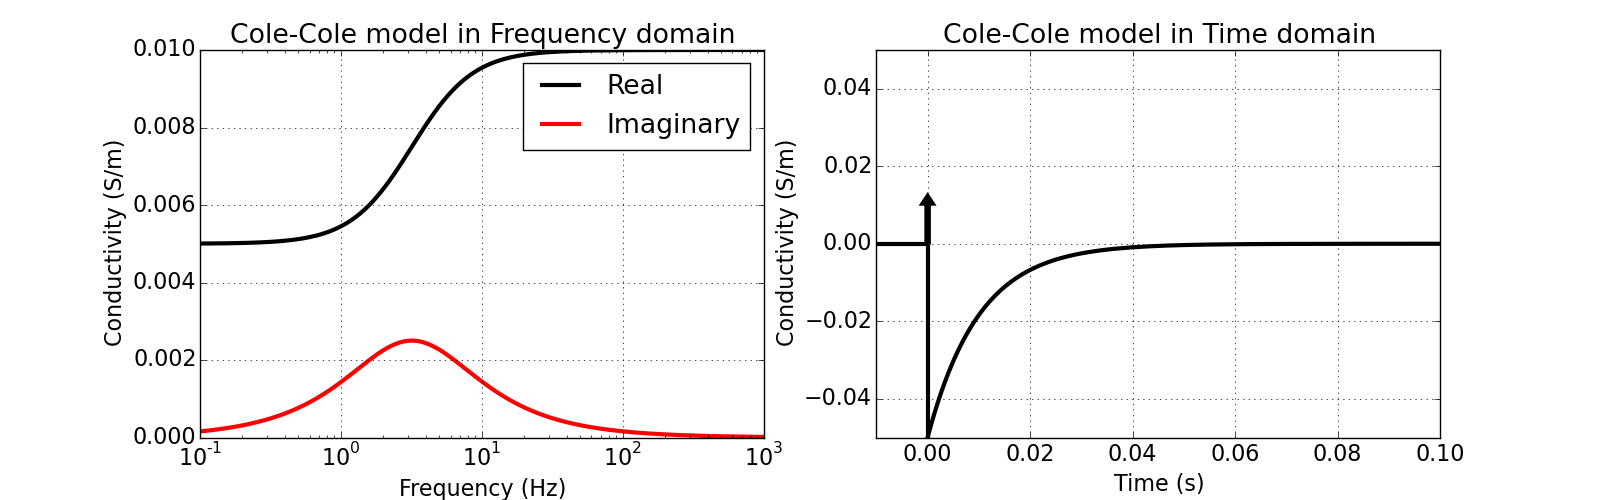
\includegraphics[width=1.0\textwidth]{figures/FDandTDCole.png}
  \caption{Cole-Cole model in frequency domain (a) and time (b) domain. }
  \label{Fig:FDandTDCole}
\end{figure}
\clearpage

%%% ===========================================================================
%%% SUBSECTION

\subsection{Convolution approach}
Consider Maxwell's equations in time domain:
\begin{equation}
  \curl{\e} = -\frac{\partial \b}{\partial t}
  \label{eq: total_farad}
\end{equation}
\begin{equation}
  \curl{\frac{1}{\mu}\b} - \j= \j_{s},
  \label{eq: total_coulomb}
\end{equation}
where $\e$ is the electric field ($V/m$), $\b$ is the magnetic flux density ($Wb/m^2$) and $\mu$ is the magnetic permeability ($H/m$). Here $\j$ is the conduction current. In the frequency domain the current density $\J$ is related to conductivity via $\J(\omega) = \sigma(\omega)\E(\omega)$ where $\E$ is the electric field. Substituting equation (\ref{eq: sigma_freq}) yields:
\begin{equation}
	\J(\omega) = \siginf\E(\omega)+\vec{J}^{pol}(\omega),
\end{equation}
where the polarization current($\J^{pol}(\omega)$) is defined as 
\begin{equation}
  \J^{pol}(\omega) = \dsig(\omega) \E(\omega)
\end{equation}.
Converting this relationship to time domain using a Fourier transform yields:
\begin{equation}
	\j(t) = \sigma(t)\otimes \e(t),
	\label{eq: ohmslaw1}
\end{equation}
where $\otimes$ indicates time convolution. For causal signals, which is defined when $t \ge 0$, convolution between $a(t)$ and $b(t)$ can be written as
\begin{equation}
	a(t) \otimes b(t) = \int_0^t a(u) b(t-u) du.
	\label{eq: convolution}
\end{equation}
That is the current density depends upon the previous history of the electric field. Substituting equation (\ref{eq: sigma_time}) yields:
\begin{equation}
	\j(t) = \siginf\e(t) + \dsig(t)\otimes\e(t) = \siginf\e(t) + \j^{pol}(t),
	\label{eq: ohmslaw2}
\end{equation}
where $\j^{pol}(t) = \dsig(t)\otimes\e(t)$.

As an example, we consider a chargeable block that is subjected to a constant electric field, $\e^{ss}$ (Figure ~\ref{Fig:ChargeableBlock}). The superscript $ss$ stands for steady-state. We assume the electric field does not change due to a chargeable body thus, $\e(t) = \e^{ss}u(t)$. Following \cite{Smith1988a}, the first term in equation (\ref{eq: ohmslaw2}) can considered as the current density if there were no polarization effects: fundamental current, $\j^{F}(t)=\siginf \e^{ss}u(t)$. By using Cole-Cole model with $c=1$  and evaluating convolution in the polarization current density, we obtain
\begin{equation}
	\j^{pol}(t) = -\eta\siginf [1-e^{-\frac{t}{(1-\eta)\tau}}]\e^{ss} = -\peta(t)\siginf\e^{ss}
	\label{eq: IPdensity}
\end{equation}
with the final value at $t = \infty$ yielding $\j^{pol}=-\eta\siginf\e^{ss}=-\eta\j^{ss}$ thus, $\eta = -\frac{\j^{pol}}{\j^{ss}}$, where $\j^{ss}=\siginf \e^{ss}$. That is, the chargeability can be considered as a fraction of the fundamental and steady-state current at the infinite time when the system reaches to the steady-state for the polarization charge builud up. However on the other times, this fraction changes in time. In general case,  we have the total current:
\begin{equation}
	\j(t) = \j^{F}(t) + \j^{pol}(t) = (1-\peta(t))\j^{ss},
  \label{eq: ohmslaw3}
\end{equation}
where the pseudo-chargeability ($\peta$) is defined as 
\begin{equation}
  \peta(t) = -\frac{\j^{pol}}{\j^{ss}} 
  \label{eq: pseudochargeability_ss}
\end{equation}
The pseudo-chargeability changes in time and end its values at t = 0 and $\infty$ are 0 and $\eta$, respectively. Here $\sigma_0=(1-\eta)\siginf$ indicates conductivity at zero frequnecy.  Figure ~\ref{Fig:Convolution_es} shows the convolution between $\sigma(t)$ and $\e(t)$. Due to the polarization currents, the total current decreases after the switch on, and it reaches to the steady state at certain late time. The reason why the total current decrease is because the minus values in time dependent conductivity ($\sigma(t)$) when $t>0$ as shown in Figure \ref{Fig:FDandTDCole}b. 

Based on this analysis, we can obtain some insights about the conventional linearization in electrical field IP (EIP) and magnetic field IP (MIP) cases (\cite{seigel1959,seigel1974}), which uses both ends of complex conductivity in frequency domain: $\sigma_0$ and $\siginf$. We can define an effective conductivity as
\begin{equation}
	\sigma_{eff}(t) = \frac{\j(t)}{\e^{ss}} = \siginf(1-\peta(t)) = \siginf + \delta\sigma(t).
  \label{eq: sigeff}
\end{equation}
For $t \rightarrow \infty$, $\peta\rightarrow \eta$ (the intrinsic chargeability) and $\sigma_{eff} = \sigma_0 = \siginf(1-\eta)$, which is well used result.
Conversely, based on equation (\ref{eq: sigeff}), we define an perturbed conductivity as
\begin{equation}
  \delta\sigma(t) = -\siginf\peta(t) =\frac{\dsig(t)\otimes \e(t)}{\e^{ss}}.
  \label{eq: sigpert}
\end{equation}
Then we can rewrite equation (\ref{eq: ohmslaw3}) as
\begin{equation}
  \j(t) = (\siginf + \delta\sigma(t))\e(t).
\end{equation}
This is a principal statement of the linearization in time domain EIP and MIP responses, since it allows us to expand Maxwell's operator in terms of $\sigpert(t)$ for each time channel. Although the assumption about constant electric field allows us to have some insights about the polarization due to a chargeable body; however, it is not directly applicable to the general cases where the electric field changes due to not only the chargeable body, but also the conductive or resistive body. Therefore, this assumption should be released, and this will be treated later.

\begin{figure}[htb]
  \centering
  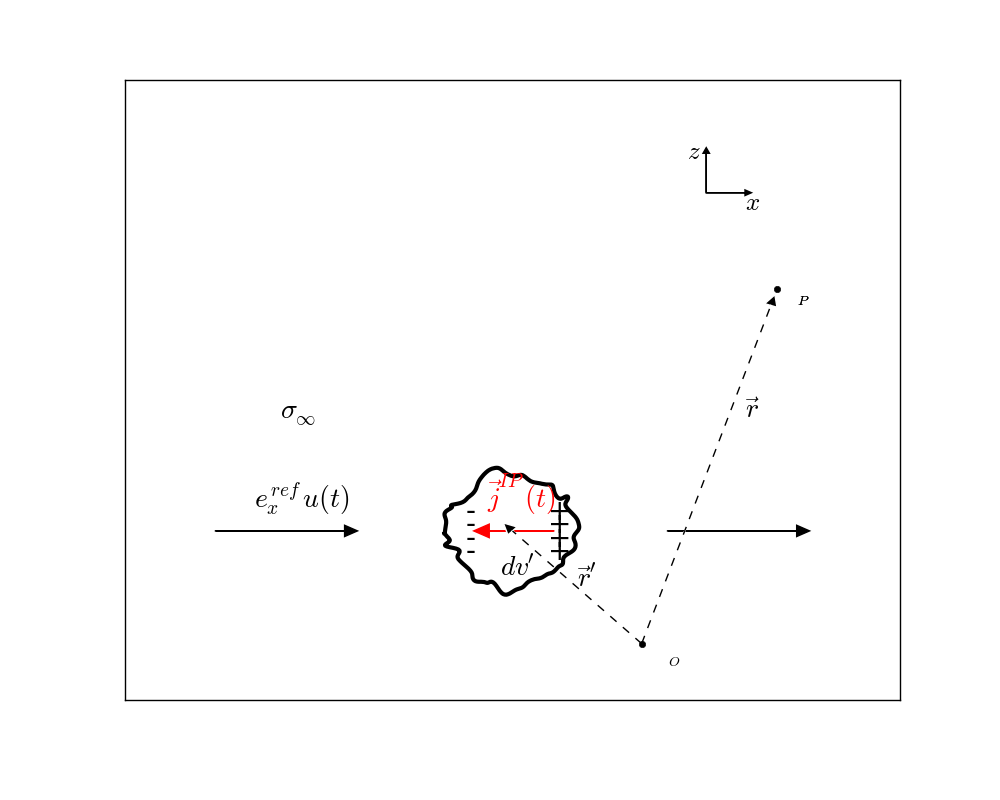
\includegraphics[width=0.6\textwidth]{figures/ChargeableBlock.png}
  \caption{A chargeable block with the complex conductivity, which is subjected to a constant electric field, $\e^{ss}$.}
  \label{Fig:ChargeableBlock}
\end{figure}
\begin{figure}[htb]
  \centering
  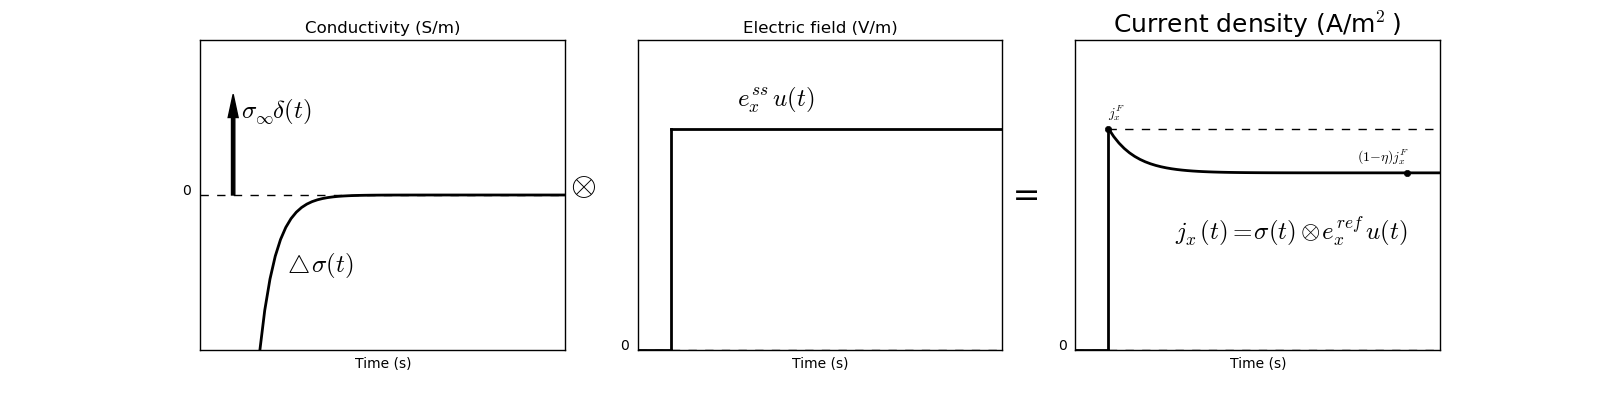
\includegraphics[width=1.0\textwidth]{figures/Convolution_es.png}
  \caption{Convolution of time dependent conductivity ($\sigma(t)$) and step-on electric field in $x$-direction ($e^{ss}_x$). }
  \label{Fig:Convolution_es}
\end{figure}

\clearpage
%%% ===========================================================================
%%% SUBSECTION

\subsection{Decomposition of EM responses}
The basic ideas and notation presented thus far form the foundation of more general cases for grounded and airborne IP measurements. The difference arises because diffusion of the fields into the subsurface need to be taken into account and also electric fields due to the polarization can become important. As in \cite{Smith1988a}, we let total fields as $\e = \e^{F} + \e^{IP}$, $\b = \b^{F} + \b^{IP}$ and $\j = \j^{F} + \j^{IP}$, where superscript $F$ indicates fundamental and $IP$ is induced polarization.
Substituting into equations (\ref{eq: total_farad}) and (\ref{eq: total_coulomb}) yields the following sequences:
\begin{equation}
  \curl({\e^{F}+\e^{IP}}) = -\frac{\partial}{\partial t} (\b^{F}+\b^{IP}),
\end{equation}
\begin{equation}
  \curl\frac{1}{\mu}(\b^{F}+\b^{IP}) - (\j^{F}+\j^{IP})= \j_{s}.
\end{equation}
By canceling out vectors associated with $EM$ terms, we have
\begin{equation}
  \curl \e^{IP} = -\frac{\partial \b^{IP}}{\partial t},
  \label{eq: eq_secondary_farad}
\end{equation}
\begin{equation}
  \curl{\frac{1}{\mu}\b^{IP}} = \j^{IP}.
  \label{eq: eq_secondary_coulomb}
\end{equation}
In addition, associated $EM$ equations can be written as
\begin{equation}
  \curl \e^{F} = -\frac{\partial \b^{F}}{\partial t},
  \label{eq: eq_primary_farad}
\end{equation}
\begin{equation}
  \curl{\frac{1}{\mu}\b^{F}} -\j^{F} = \j_s.
  \label{eq: eq_primary_coulomb}
\end{equation}
Here
\begin{equation}
  \j^{F} = \siginf\e^{F},
  \label{eq: jF}
\end{equation}
\begin{equation}
  \j^{IP} = \siginf\e^{IP} + \j^{pol}.
  \label{eq: jIP}
\end{equation}
Note that the IP current density, $\j^{IP}$ is the summation of the polarization current and $\siginf\e^{IP}$. Previously in convolution approach, we did not have this term because we assumed constant electric field ($\e(t) = \e^{ss}u(t)$). However, in general case, we need to consider this extra term due to polarization charge build up in the electric field.

Let $F[\cdot]$ denote operator associated with Maxwell’s equations and let $d$ denote the observed electromagnetic field thus, this incldues both EM and IP effects. Keeping the same notation, we also write $d = d^{F} + \dip$. Therefore, we define IP datum as
\begin{equation}
	\dip = d - d^{F} = F[\siginf\delta(t)+\dsig(t)]-F[\siginf\delta(t)].
    \label{eq: IPdatum_syn}
\end{equation}
This subtraction process acts as an EM decoupling process, which reduces the EM effects in the measured responses. This formed the basics of work by \cite{routh2001}. Thus, assuming that we have a reasonable estimation for the distribution of $\siginf$ in 3D space, we can identify  IP datum, which are embedded in the observed responses. 
\bigskip
\todo[inline, color=yellow!40]{
\noindent\textbf{Questions 1: Is it true that we have only IP effect with this subtraction process?} ç\newline
Doug: We need to show under what circumstances this is true. It is tied in with the statement that $\curl\e^{IP} = 0$. i.e. the polarization decays do not cause EM induction. Handling this matter here simplified much of the following paper.\medskip\newline
\textcolor{blue}{Answer: I think that EM induction due to polarization decays are also IP effect, which is due to time dependent conductivity.}
}

% \bigskip
% \todo[inline, color=green!20]{
% \noindent\textbf{Issue1: Naming issues of $\vec{p}$ and $\j^{IP}$. How about $\j^{pol}$?}
% Solved: we use $\j^{pol}$
% }

%%% ===========================================================================
%%% SUBSECTION

\subsection{Thoughts on IP and polarization currents}
With consideration of time dependent conductivity, current density was written as
\begin{eqnarray*}
    \j(t) = \siginf\e(t)+\j^{pol}(t),
\end{eqnarray*}
where $\j^{pol}(t)=\dsig(t)\otimes\e(t)$. Or this can be rewritten as
\begin{equation*}
    \j(t) = \j^{F}(t) + \j^{IP}(t),
\end{equation*}
where $\j^{F}(t)=\siginf\e^{F}(t)$ and
\begin{eqnarray}
		\j^{IP}(t) = \siginf\e^{IP}(t) + \j^{pol}(t).
        \label{eq: jip_with_ja}
\end{eqnarray}
We first consider the polarization current ($\j^{pol}$). Using the integral equation form for equations (\ref{eq: eq_secondary_farad} and \ref{eq: eq_secondary_coulomb}), $\e^{IP}$ and $\b^{IP}$ can be expressed as 
\begin{equation}
    \e^{IP}(\vec{r}; t) = \int_{\Omega} \bar{\mathbf{G}}^{E}(\vec{r}, \vec{r}_s)\otimes\j^{pol}(\vec{r}_s; t) d\vec{r}_s,
\end{equation}
\begin{equation}
    \b^{IP}(\vec{r}; t) = \int_{\Omega} \bar{\mathbf{G}}^{B}(\vec{r}, \vec{r}_s)\otimes\j^{pol}(\vec{r}_s; t) d\vec{r}_s,
\end{equation}
where $\bar{\mathbf{G}}^{E}$ and $\bar{\mathbf{G}}^{B}$ are electric and magnetic green's tensors. Here $\j^{pol}$ can be considered as a source term. Assuming that we know the polarization current and the above green's tensors, we can compute $\e^{IP}$ and $\b^{IP}$ by evaluating those integrals. This emphasizes the importance of the polarization current for the IP responses. In convolution approach, $\j^{pol}$ was defined as
\begin{equation}
    \j^{pol}(t) = -\peta(t)\siginf\e^{ss}=-\peta(t)\j^{\ ref},
\end{equation}
where the reference current density is $\j^{\ ref} = \j^{ss} = \siginf\e^{ss}$.
This allows to build up a conceptual model of the IP responses: an IP body acts like a dipole which has opposite direction to reference current density, and proportional to $\peta$. This conceptual model is analogous to Seigel's one (\cite{seigel1959}).

Second, we treat IP current density $\j^{IP}$. Based on equation (\ref{eq: eq_secondary_coulomb}), we can apply Biot-Savart law:
\begin{equation}
  \b^{IP}(\vec{r}; t) = \frac{\mu_0}{4\pi}\int_{\Omega}  \frac{\j^{IP}(\vec{r}_s; t)\times\hat{r}}{|\vec{r}-\vec{r}_s|^2}d\vec{r}_s. 
\end{equation}
This equation shows that  we can compute $\b^{IP}$ using $\j^{IP}$. Different from the magnetic greens tensor ($\bar{\mathbf{G}}^B$), a kernel in Biot-Savart law is purely geometric. However we need to know the additional term $\siginf\e^{IP}$ to compute $\b^{IP}$ using Biot-Savart law. This is caused by difference between $\bar{\mathbf{G}}^B$ and kernel function of Biot-Savart law. Both approaches can be useful in spite of some different features. These two kernels can be same for a specific case where we do not have any conductivity contrast in $\siginf$ without any EM induction effect. Biot-savart law can have different form (CITE):
\begin{equation}
  \b^{IP}(\vec{r}; t) = \frac{\mu_0}{4\pi}\int_{\Omega}  \frac{\vec{\nabla}_s \times \j^{IP}(\vec{r}_s; t)}{|\vec{r}-\vec{r}_s|}d\vec{r}_s.
  \label{eq: Biot}
\end{equation}
If we let $\e^{IP} = -\grad\phi^{IP}$ and $\siginf$ is constant, then we can substitute $\j^{IP}$ in above equation as $\j^{pol}$ because $\curl \grad \phi^{IP} = 0$. This result shows that we do not need to know $\siginf \e^{IP}$ term to compute $\b^{IP}$ for this specific case. 

We have recognized that $\j^{IP}$ can be a fundamental element of understanding IP responses. In order to get some insights of $\j^{IP}$, we decompose $\j^{IP}$ as
\begin{equation}
    \j^{IP}(t) = \siginf\e^{IP}(t) + \dsig(t)\otimes\e^{F}(t)+ \dsig(t)\otimes\e^{IP}(t).
    \label{eq: jip_three}
\end{equation}
For notational convenience, we respectively refer to $\siginf\e^{IP}(t)$, $\dsig(t)\otimes\e^{F}(t)$ and $\dsig(t)\otimes\e^{IP}(t)$ as $\j^{IP}_1$, $\j^{IP}_2$ and $\j^{IP}_3$. Characteristics of each current density are following. We start with $\j^{IP}_1$. This is defined everywhere. This is the term makes a difference between $\j^{IP}$ and $\j^{pol}$. Recalling Smith’s approximate convolution approach (\cite{Smith1988a}), he assumed $\j^{IP}_1$ and $\j^{IP}_3$ are negligible, which makes $\j^{IP} = \j^{pol}$. In his case, an IP body was surrounded by the free space and $\eta \ll 1$.  However, in general case where the background medium is not free space, this term may not be negligible in that $\j^{IP}_2$ and $\j^{IP}_3$ are only defined in the IP body because $\dsig(t)$ is zero except for the IP body. This shows that $\j^{IP}_2$ is going to be the main term of $\j^{IP}$ in the IP body as the conductivity of background medium and $\eta$ decrease. In addition, $\j^{IP}_3$ might be negligible when we have small $\eta$. However, it is hard to suggest that when we have considerable $\eta$, since this is convoluted property of $\e^{IP}$ and $\dsig(t)$.

%%% ===========================================================================
%%% SECTION 3. MAIN
%%% ===========================================================================

\section{Linearization of IP responses}

%%% ===========================================================================
%%% SUBSECTION

\subsection{Linearization in EIP and MIP}
For the linearization of IP response, it is useful to think in terms of EIP or MIP experiment where we apply a direct current into the ground. We use step-on waveform. Neglecting induction, $F[\siginf]=F_{DC}[\siginf] \rightarrow \e^{ss}_{\siginf}$, where $F_{DC}[\cdot]$ indicates steady-state Maxwell's operator. Recalling the definitions of $\delta\sigma$ and $\sigma_{eff}$ that we have made in convolution approach, we approximately rewrite total current density, $\j$ as
\begin{eqnarray}
	\j(t) \approx (\siginf + \delta\sigma(t))\e(t) = \sigma_{eff}(t)\e(t).
  	\label{eq: ohmslaw4}
\end{eqnarray}
The perturbed conductivity and effective conductivity were defined as $\delta\sigma = \frac{\dsig(t)\otimes\e(t)}{\e^{ss}}$ and $\sigma_{eff} = \frac{\j}{\e^{ss}}$. Considering that we use step-on waveform, this is reasonable approximation, since $\e(t)\approx \e^{ss}u(t)$ when $\eta \ll 1$. By substituting $\vec{e}^{ss}$ in $\delta\sigma(t)$ with $\vec{e}(t)$, equation (\ref{eq: ohmslaw4}) can be converted to an equality equation. By substituting the constant electric field $\e^{ss}$ as $\e_{\siginf}^{ss}$, we let
\begin{equation}
  \dsig(t)\otimes\e(t) = \j^{pol}(t) \approx \delta\sigma(t)\e(t).
  \label{eq: jpol_approx}
\end{equation}
Based on this assumption for EIP problem, IP response at any time $t>0$ can be expressed as $F_{DC}[\sigma_{eff}(t)]$. Then we make Taylor expansion and obtain
\begin{equation}
  F_{DC}[\siginf + \delta\sigma_i] = F_{DC}[\siginf] + \frac{\partial F_{DC}[\siginf]}{\partial\siginf}\delta\sigma_i + O(\delta\sigma_i^2),
  \label{eq: TaylorDC}
\end{equation}
where subscript $i$ indicates $i^{th}$ time channel. By ignoring the second order term in equation (\ref{eq: TaylorDC}) with some linear algebra, we obtain the IP datum at $i^{th}$ time channel:
\begin{equation}
  \dip_i = F_{DC}[\siginf + \delta\sigma_i] - F_{DC}[\siginf] \approx -\frac{\partial F_{DC}[\siginf]}{\partial log(\siginf)}\peta_i,
  \label{eq: EIPlinear1}
\end{equation}
where $\peta_i = -\frac{\sigpert_i}{\siginf}$. This constructs a general formulation of linear inverse problem in EIP (\cite{Yuval1997}, \cite{Hordt2006}). In addition, this still applicable to MIP case (\cite{seigel1974,Chen2003}).

Conversely, all of our derivations has been done for a step-on current. Then what happen if the data are measured in the off-time? Off time response ($\dip_{off}$) can be simply computed using on-time response ($\dip_{on}$), using the following relationship:
\begin{equation}
  \dip_{off}(t) = \dip_{on}(t=\infty) - \dip_{on}(t) = F_{DC}[\sigma_0] - \dip_{on}(t),
\end{equation}
where $\sigma_0 = \siginf(1-\eta)$, which is the low frequency limit of Cole-Cole model. This indicates that we can still use equation (\ref{eq: EIPlinear1}), because the off-time result is directly related to the on-time as illustrated in Figure ~\ref{Fig:EIPcurve}. However, in practice, the input current waveform can be arbitrary as shown in Figure \ref{Fig:Oscillating_e}. We let a current waveform as $I_0w(t)$, where $I_0$ is the magnitude of the current and $w(t)$ is that of the time dependency. The maximum charging will occur when a uniform field has been applied for a duration $t \gg \tau$. Let $\e^{ss}$ represents the steady state field associated with $I(t) = I_0u(t)$. In this case, the assumption that we made for $\j^{pol}$ (equation (\ref{eq: jpol_approx})) may not be reasonable, because the total electric field, $\e(t)$ can dynamically change due to $w(t)$ so that the electric field at $i^{th}$ time channel, $\e_i$ can be quite different from $\e^{ss}$ as shown in Figure ~\ref{Fig:Oscillating_e}. Therefore, for this general waveform, it is not straight forward to linearize EIP responses with the current framework. 

\begin{figure}[htb]
  \centering
  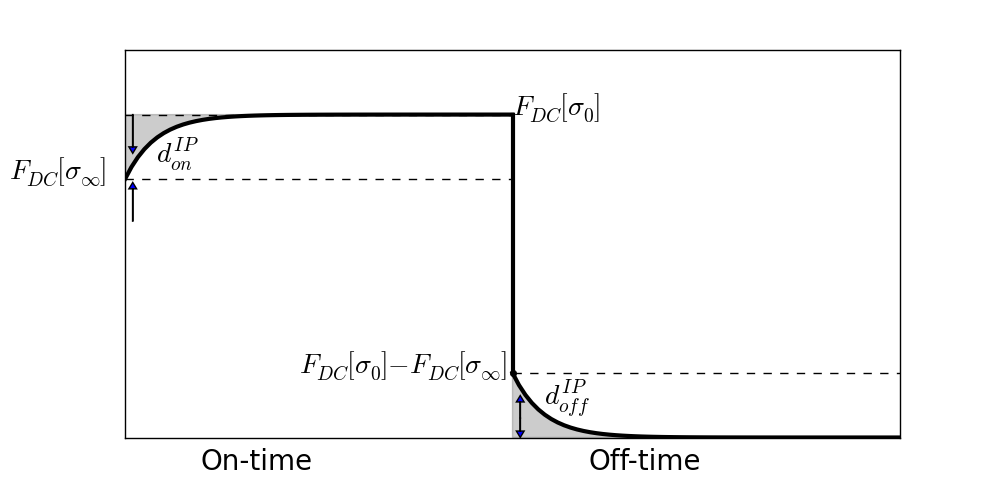
\includegraphics[width=0.8\textwidth]{figures/EIPcurve.png}
  \caption{Time domain EIP curve. }
  \label{Fig:EIPcurve}
\end{figure}
\begin{figure}[htb]
  \centering
  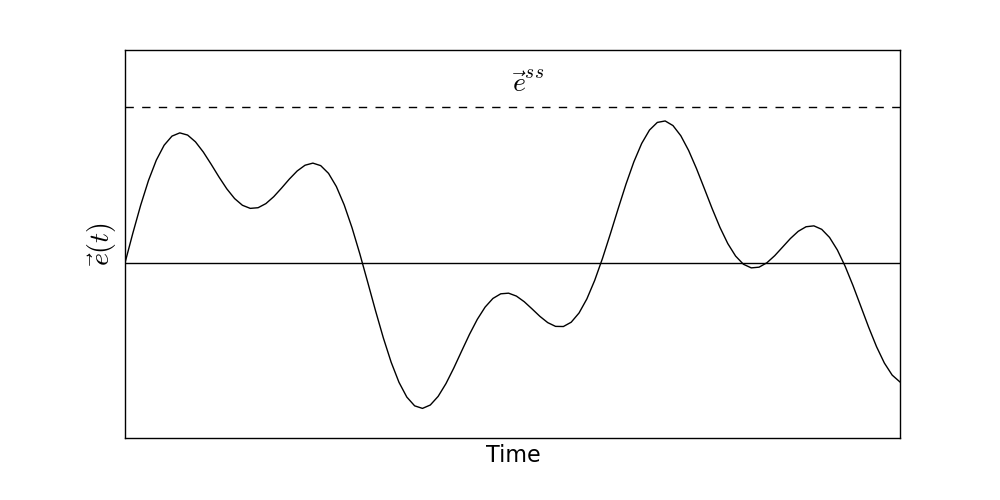
\includegraphics[width=0.8\textwidth]{figures/Oscillating_e.png}
  \caption{Conceptual diagram of oscillating electric field.}
  \label{Fig:Oscillating_e}
\end{figure}
\clearpage

%%% ===========================================================================
%%% SUBSECTION
\subsection{Linearization in TEM-IP}
In previous two sections, we have treated the linearization of the IP responses without consideration of the EM induction effect. The fundamental responses of EIP and Mip cases with step-on or step-off waveform were independent on time thus, any time dependent responses are due to the IP effect. However, ignoring EM induction effect may not be easonable, in particular, inductive source TEM case can be a representative example because the EM induction is the driving force of the system. Therefore, we need to release this assumption to handle those situations where we cannot ignore EM induction effect. Now a principal difference from the steady-state IP case is not only the IP-related fields, but also the fundamental fields can be time dependent. However, we still want to use a similar linearization approach from the steady-state case, which expands Maxwell's operator in terms of $\sigpert(t)$. A significant problem here is the EM induction term ($\frac{\partial \b}{\partial t}$) in equation (\ref{eq: total_farad}). This term makes a coupling between the current and previous time channels, thus expanding this operator in terms of $\sigpert(t)$:
\begin{equation*}
  F[\siginf+\dsig(t)] \approx F[\siginf] + \frac{\partial F[\siginf]}{\partial \siginf}\sigpert
\end{equation*}
is not valid. Accordingly, we need a different approach to tackle this problem, although most of the principal methodologies used in the EIP and MIP case can be similarly applied.

Nonetheless, our goal is stil similar as before: we want to express $\dip$ as a function of the pseudo-chargeability $(\peta(t))$ in time. Therefore, we can have a form of linear equation like $\dip(t) = -J[\peta(t)]$, where $J[\cdot]$ is a linear operator, which is independent on time. For this, we consider a general system whether we can consider either grounded or inductive source and any types of measured field. Let the total electric field, $\e(t)$ can be approximated as
\begin{equation}
  \e(t) \approx \e^{\ ref}w^e(t),
  \label{eq: e_with_eref}
\end{equation}
where $w^e(t)$ is defined as:
% \begin{equation}
%   w^e(t) = \frac{\e(t)\cdot\e^{\ ref}}{\e^{\ ref}\cdot\e^{\ ref}}.
%   \label{eq: we}
% \end{equation}
\begin{equation}
  w^e(t) = \left\{ 
  \begin{array}{l l}
    w^{ref}(t) & w^{ref}(t) \ge 0 \\
    0 & \text{if } w^{ref}(t) < 0, 
  \end{array}\right.
  \label{eq: we}
\end{equation}
with
\begin{equation}
  w^{ref}(t) = \frac{\e(t)\cdot\e^{\ ref}}{\e^{\ ref}\cdot\e^{\ ref}}.
  % \label{eq: we}
\end{equation}
Here $w^{ref}(t)$ is a dimensionless function that prescribes the time history of the electric field at each location and the reference electric field ($\e^{\ ref}$) is an appropriate scaling for the electric field, which is independent on time. 
This indicates that the direction of the electric field does not change in time. 
In addition, by the definition of $w^e(t)$, we projects negatives values of  $w^{ref}(t)$ to zero.
Note that this assumption is only applied to the second term on right-hand side of equation (\ref{eq: jIP}). 
Substituting this into equation (\ref{eq: jIP}) yields
\begin{eqnarray*}
  \j^{IP}(t) \approx \siginf\e^{IP}(t) + \frac{\dsig(t)\otimes w^e(t)}{\siginf}\j^{\ ref},
\end{eqnarray*}
where the reference current density is defined as
\begin{equation}
  \j^{ref} = \siginf\e^{\ ref}.
\end{equation}
Letting pseudo-chargeability as
\begin{equation}
    \peta(t) = -\frac{\dsig(t)\otimes w^e(t)}{\siginf} \approx -\frac{\j^{pol}}{\j^{\ ref}},
    \label{eq: pseudochargeability}
\end{equation}
we obtain
\begin{eqnarray}
  \j^{IP}(t) = \siginf\e^{IP}(t) + \j^{pol}(t) \approx \siginf\e^{IP}(t) -\j^{\ ref}\peta(t).
  \label{eq: jip_EMIP}
\end{eqnarray}
A physical insight about the pseudo-chargeability is that a fraction of polarization current and reference current. Because the reference current is time-independent property, any time-dependency in the pseudo-chargeability is from the polarization current. Using Helmholtz decomposition, $\e$ can be decomposed as $\e=-\vec{a}-\grad\phi$, where $\vec{a}$ and $\phi$ is electric vector and scalar potentials, respectively and $\div\vec{a}=0$. Physically, those two terms indicate charge-build up and EM induction effects, which induce galvanic and vortex currents, respectively. So, $\e^{IP}$ can be decomposed as
\begin{equation}
  \e^{IP}=-\vec{a}^{IP}-\grad\phi^{IP}.
\end{equation}
Now we make an another assumption:
\begin{equation}
  \e^{IP} \approx  \e^{IP}_{approx} = -\grad\phi^{IP},
  \label{eq: eip_approx}
\end{equation}
which means $\e^{IP}$ term in equation (\ref{eq: jip_EMIP}) is dominated by galvanic effect ($\frac{\partial\b^{IP}}{\partial t}\approx 0$). First taking $\div$ to equation (\ref{eq: jip_EMIP}) then by substituting  $\e^{IP}$ with equation (\ref{eq: eip_approx}) with some linear algebra, we obtain
\begin{equation}
  \phi^{IP}(t) \approx -[\div \siginf\grad]^{-1}\div\j^{\ ref}\peta(t).
  \label{eq: phiIPapprox_general}
\end{equation}
By taking $\grad$ to this equation we have
\begin{equation}
    \e^{IP}_{approx} = \grad[\div \siginf\grad]^{-1}\div\j^{\ ref}\peta(t).
    \label{eq: eip_approx_full}
\end{equation}
Thus, the electric field due to the IP effect can be expressed as a function of $\peta(t)$ in time.

The observd data can be $\b$ or $\frac{\partial \b}{\partial t}$ in some cases thus, we need to compute $\b^{IP}$ or $\frac{\partial \b^{IP}}{\partial t}$. For this, we first compute $\j^{IP}$ then use Biot-Savart law to compute $\b^{IP}$ or $\frac{\partial \b^{IP}}{\partial t}$. Substituting equation (\ref{eq: phiIPapprox_general}) into equation (\ref{eq: jip_EMIP}), approximated IP current density, $\j^{IP}_{approx}$ can be expressed as
\begin{equation}
  \j^{IP}(t) \approx \j^{IP}_{approx} = -\bar{S}\siginf\e^{\ ref}\peta(t),
  \label{eq: jip_approx}
\end{equation}
where
\begin{equation}
  \bar{S} = -\siginf\grad[\div \siginf\grad]^{-1}\div+\bar{I}
\end{equation}
and $\bar{I}$ is an identity tensor. Then by using Biot-Savart law we have:
\begin{equation}
  \b^{IP}_{approx}(\vec{r}; t) = -\frac{\mu_0}{4\pi}\int_{\Omega}  \frac{\bar{S}\e^{\ ref}(\vec{r}_s)\times\hat{r}}{|\vec{r}-\vec{r}_s|^2}\peta(t)d\vec{r}_s.
  \label{eq: BiotbIP_approx}
\end{equation}
By taking time derivative to the above equation we have
\begin{equation}
  \frac{\partial\b^{IP}_{approx}}{\partial t}(\vec{r}) = -\frac{\mu_0}{4\pi} \int_{\Omega}  \frac{\bar{S}\e^{\ ref}(\vec{r}_s)\times\hat{r}}{|\vec{r}-\vec{r}_s|^2}\frac{\partial}{\partial t}\peta(t)d\vec{r}_s.
  \label{eq: BiotbIPdt_approx}
\end{equation}
Both equations (\ref{eq: BiotbIP_approx}) and (\ref{eq: BiotbIPdt_approx}) are function of $\peta(t)$, and the time dependency only rises from $\peta(t)$. 
To summarize, with the assumption that $\e^{IP}$ is mostly galvanic, we show that electromagnetic fields due to IP effects can be expressed as instantaneous property, which have linear relationship with $\peta(t)$. Therefore, $\dip$ responses, which can be any type of electromagnetic fields, can be represented as $\dip(t) = -J[\peta(t)]$. In discretized space this can be expressed as
\begin{equation}
  \mathbf{d}^{IP}_i = -\mathbf{J}\peta_i,
  \label{eq: dIP_lineareq}
\end{equation}
where $\mathbf{J}$ is corresponding sensitivity matrix and the subscript $i$ indicates $i^{th}$ time channel. Boldface of upper and lower cases indicate a matrix and column vector in discretized space. Since $\dip$ can be any types of electromagnetic fields, our approach to linearize time domain IP responses is applicable for any types of TEM surveys, whereas some details for practical application might be somewhat different. However, the fundamental concept will be same.

On the other hand, we must carefully investigate the assumptions that we have made to formulate this linear relationship, and a fundamental characteristics of what we are recovering; thus, we need to identify four fundamental points. We made two assumptions: (a) we know exact background conductivity model ($\siginf$). (b) Inductive effect in $\e^{IP}$ is negligible. (c) $\dsig(t)\otimes \e(t) = -\peta(t)\j^{\ ref}$, In addition, (d) we recognized that $\peta(t)$ is convoluted property with $\e(t)$ and distributed IP parameters. Those four points are not trivial to be validated in physical or mathematical ways; thus each of them should be carefully tested with numerical experiments for different types TEM surveys like grounded or inductive source TEM methods and different conductivity structures.

%%% ===========================================================================
%%% SUBSECTION
\subsection{Discussions}
%%% ===========================================================================
%%% SUBSUBSECTION
\subsubsection{Choice of reference electric field}
We first consider the choice of the reference electric field for the grounded source IP case. Although we have the EM induction effect for the grounded source case, here we assume the EM induction effect is minor to the galvanic effect. Thus, the time behaviour of the fundamental electric field with step-on and -off waveform will be same as that of the input current as shown in Figure \ref{F:DCEM_F_current}a. The choice of the reference electric field in this case is intuitive, because the fundamental electric field is constant on on-time period. That is, we choose the electric field at the steady-state with $\siginf$ ($\e^{ss}_{\siginf}$) as $\e^{\ ref}$. This will be a reasonable choice for the grounded source case even if we consider EM induction effect. 

A fundamental difference from galvanic and inductive source arises from the property, $\div\j_s$.  If this is zero then it is inductive source or if not, it is galvanic source. In order to get some insight, consider DC problem for inductive source:
\begin{eqnarray*}
    -\div\j^{ss} = \div\j_s = 0, \\
    \div \siginf \grad \phi^{ss}_{\siginf} = -\div\j_s = 0.
\end{eqnarray*}
Since the right-hand side of the above equation is zero, thus, $\phi^{ss}_{\siginf}$ = 0 and $\e^{ss}_{\siginf}=0$. This shows that there are no DC fields for inductive source case. 

For the inductive source case, we cannot ignore the EM induction effect because it is the driving force of the system. We consider the magnitude of the electric field at a single pixel in the earth with a step-off waveform. As shown in Figure \ref{F:DCEM_F_current}b, this will start from zero, reaches to the maximum then decays. We choose the fundamental electric field at the maximum as the reference electric field. Mathematical representation of this choice can be written as 
\begin{equation}
  \e^{\ ref} = \e^{F}_{max} = \e^{F}(t) \otimes \delta(t-t^{max}),
\end{equation}
where $t^{max}$ is the time when the magnitude of the fundamental electric fields reach to the maximum. Note that $t_{max}$ is variable in 3D space, since the electric field at each pixel in 3D space can have different time decaying feature due to the source location and conductivity distribution. The reason why we define the reference electric field is due to the approximation for the polarization currents: $\j^{pol} = -\j^{\ ref}\peta$, where $\j^{\ ref} = \siginf \e^{\ ref}$. An important reasoning behind this approximation is that the amplitude of the polarization current is proportional to the reference current, and that of the direction does not change dramatically in time. Therefore, choosing the fundamental electric field at the time when it reaches to the maximum indicates that the amplitude of the polarization current is proportional to the reference current at this time, and the direction of of the polarization current is similar to that of the reference current. This explanation is applicable for both galvanic and inductive source IP cases. The reference electric field for the galvanic source cases can be the fundamental electric field at the maximum as well ($\e^{F}_{max}$). 

\begin{figure}[htb]
  \centering  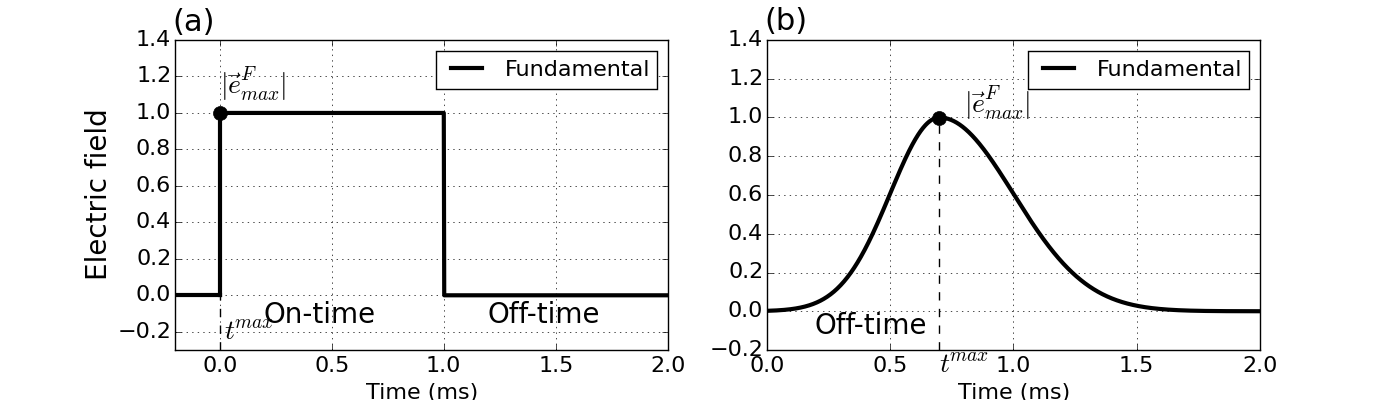
\includegraphics[width=1.0\textwidth]{figures/DCEM_F_current.png}
  \caption{Conceptual diagram for the amplitude of the fundamental electric fields. (a) Galvanic and (b) inductive source IP cases.}
  \label{F:DCEM_F_current}
\end{figure}

\todo[inline, color=green!20]{
\noindent\textbf{Constant ramp for the inductive source: obtain same analogy for grounded source case (constant electric field)}\newline\newline
Polarization charge build up reaches to the steady state
}
\clearpage

%%% ===========================================================================
%%% SUBSUBSECTION
\subsubsection{Revisitation of EIP and MIP}
In previous section, we suggested a linearization methodology, which can be applied to general TEM problems. Using this methodology, we revisit the linearization of the IP responses in EIP and MIP cases. Recall that we had a challenge in linearization when we have general current waveform.

As we mentioned on previous section, a proper reference electric field for EIP and MIP cases can be $\e^{ss}_{\siginf}$, so we modify equation (\ref{eq: e_with_eref}) as
\begin{equation*}
    \e(t) \approx \e^{ss}_{\siginf}w^e(t).
\end{equation*}
Then $\phi^{IP}(t)$ shown in equation (\ref{eq: phiIPapprox_general}), can be rewritten as
\begin{eqnarray*}
  \phi^{IP}(t) \approx \phi^{IP}_{approx} =  -[\div\siginf\grad]^{-1}\div\grad\phi^{ss}_{\siginf}(\dsig(t)\otimes w^e(t)) \\
               =\frac{\partial \phi^{ss}_{\siginf}}{\partial \siginf}\dsig(t)\otimes w^e(t)
\end{eqnarray*}
and finally we have
\begin{eqnarray}
    \phi^{IP}_{approx}(t) = \frac{\partial \phi^{ss}_{\siginf}}{\partial \siginf}\dsig(t)\otimes w^e(t) \nonumber\\
                 =\frac{\partial \phi^{ss}_{\siginf}}{\partial \siginf}\sigpert(t)
\end{eqnarray}
where $\sigpert(t) = \frac{\dsig(t)\otimes \e(t)}{\e^{ss}_{\siginf}}=\dsig(t)\otimes w^e(t)$ and
\begin{equation}
    \frac{\partial \phi^{ss}_{\siginf}}{\partial \siginf} = -[\div\siginf\grad]^{-1}\div\grad\phi^{ss}_{\siginf}.
    \label{eq: senseDC}
\end{equation}
Detailed derivation of equation (\ref{eq: senseDC}) in discretized space is given in appendix ??. Substituting equation (\ref{eq: pseudochargeability}) to (\ref{eq: senseDC}), we have
\begin{equation}
    \phi^{IP}_{approx}(t) = -\frac{\partial \phi^{ss}_{\siginf}}{\partial log(\siginf)}\peta(t),
    \label{eq: phiIPapprox}
\end{equation}
which is the same result from equation (\ref{eq: EIPlinear1}) for electrical potential. Therefore, we can derive same result with conventional linearization in EIP case using suggested methodology. $\e^{IP}$ can also be linearized in the same way, since we can just take gradient to the above equation and obtain $\e^{IP}$.

For MIP case, we measure the magnetic flux density, and we linearized $\b^{IP}$ by expanding Maxwell's operator. However, in this time we use the suggested linearization aproach for the general case. Modifying equation (\ref{eq: jip_EMIP}), we obtain
\begin{eqnarray}
    \j^{IP}(t) = \siginf\e^{IP}(t) + \dsig(t)\otimes w^e(t)\e^{ss}_{\siginf} \nonumber \\
            = -\bar{S}\siginf\e^{ss}_{\siginf}\peta(t).
\end{eqnarray}
Applying Biot-Savart law yields
\begin{equation}
  \b^{IP}(\vec{r}; t) = -\frac{\mu_0}{4\pi}\int_{\Omega}  \frac{\bar{S}\e^{ss}_{\siginf}(\vec{r}_s)\times\hat{r}}{|\vec{r}-\vec{r}_s|^2}\peta(t)d\vec{r}_s.
  \label{eq: BiotbIP_ss}
\end{equation}
Different from conventional linearization approach used in EIP and MIP cases, applicability of our linearization method is not limited to step-on or step-off waveform, but general. Therefore, even when we have general waveform, which can be oscillating as shown in Figure ~\ref{Fig:Oscillating_e}, the linearzation of EIP or MIP can still proceed. Furthermore, considering an oscillating input current as shown in Figure ~\ref{Fig:Oscillating_e} also supports this statement, because $|\delta(t)| \ll \siginf\eta$.

%%% ===========================================================================
%%% SUBSUBSECTION
\subsubsection{Ignoring inductive IP effect}

In constrolled-source EM (CSEM) experiments, we can have two types of sources: grounded and inductive sources. We first consider this assumption for grounded source. Ignoring inductive part of IP effect $\frac{\partial \b^{IP}}{\partial t}\approx 0$, might be reasonable for grounded source case, since galvanic effect can be dominant ($\grad\phi^{IP} \gg \vec{a}^{IP}$) in most cases, but this should be carefully tested because it depends on the conductivity structure and time. 

Different from the galvanic source, for the inductive source case, the EM induction is the main driving force of the system. Therefore, we need to be more careful when we ignore inductie IP effect. Consider a situation where we have homogeneous background conductivity model ($\siginf$=constant). Recall $\j^{IP}$ with Helmholtz decomposition:
\begin{eqnarray*}
    \j^{IP} = \siginf\e^{IP} + \dsig(t)\otimes w^{e}(t)\e^{\ ref} \\
            = -\siginf(\grad\phi^{IP}+\vec{a}^{IP}) + \dsig(t)\otimes w^{e}(t)\e^{\ ref}
\end{eqnarray*}
By taking $\div$ we have
\begin{equation*}
    -\div\siginf\grad\phi^{IP}-\div\siginf\vec{a}^{IP} = -\div\dsig(t)\otimes w^{e}(t)\e^{\ ref}.
\end{equation*}
Since $\siginf$ is constant in space, then we rewrite
\begin{equation*}
    \div\siginf\grad\phi^{IP} = \j^{pol}_{approx},
\end{equation*}
where $\div\vec{a}^{IP}=0$ and $\j^{pol}_{approx}  = \div\dsig(t)\otimes w^{e}(t)\e^{\ ref}$. Therefore, once we do not have any conductivity variation in our background conductivity model, we can obtain reasonable $\phi^{IP}$ by solving above sytem. This indicates we can compute IP responses, which are related to galvanic effect, while we still can have significant induction portion, $\vec{a}^{IP}$ in $\e^{IP}$. Note that $\div\vec{a}^{IP}=0$ does not mean $\vec{a}^{IP}=0$. Further in general case where we have conductivity constrast in the earth, $\div \siginf \vec{a}^{IP}$ may not be zero, thus the relative strength of  $\siginf \vec{a}^{IP}$ to $\j^{pol}_{approx}$ should be minor to make our assumption reasonable. Intuitively, we know that EM induction effect is going to decay faster than galvanic effect so that they are going to small in late time channels. To account for this effect, we consider Faraday's law
\begin{eqnarray*}
    \curl \vec{a}^{IP}(t) = \frac{\partial \b^{IP}(t)}{\partial t},
\end{eqnarray*}
since $\curl \grad \phi^{IP} = 0$. This tells us time varying magnetic flux density generate rotational electric field, that is $\vec{a}^{IP}$. This induced IP effect may have an influnence on polarization charge build up ($\phi^{IP}$) due to the term $\div\siginf\vec{a}^{IP}$, when we have conductivity constrast in the earth. Relative influence of this term will vary for different conductivity structures. 
In frequency domain equation, we have
\begin{equation*}
    \curl \vec{A}^{IP}(\omega) = \imath\omega\B^{IP}(\omega).
\end{equation*}
The magnitude of $\vec{A}^{IP}$ is proportional to $\omega$ in frequency domain. As $\omega$ decrease, EM induction effect gets smaller. Accordingly, $\vec{a}^{IP}$ in $\e^{IP}$ gets smaller as we move on to late time channels, thus galvanic term $\phi^{IP}$ can be dominant term in $\e^{IP}$ at certain late time channels. Those are possible situations that we are interested for IP signals and we might have some chances to apply our linearization methodology.


% which can be used in actual paper
%==============================================================================
% Due to the consideration of time dependent conductivity, current density includes convolution term (\ref{eq: ohmslaw1}), and this can make significant complexity in computing forward response of this EM system. Intuitively, inverse problem to recover distribution of time dependent conductivity can also be much more complex. Although we can directly derive inverse problem to recover 4D distribution of time dependent conductivity or distributed Cole-Cole parameters; however, we choose a linearization approach to simplify this inverse problem. Based on the experience in DC-IP inversion in  the past couple decades, we believe that the linearization approach can be a more robust solution to approach this inverse problem.

% Principal flow of linearization of time domain IP responses for inductive source has two steps: (a) The most principal component of our linearization is polarization current density, $\j^{IP}$. We linearize $\j^{IP}$ and express in terms of pseudo chargeability.  (b) Once we have $\j^{IP}$ then $\b^{IP}$ of $\frac{\partial\b^{IP}}{\partial t}$ can be computed using Biot-Savart law. Recalling that measured data for inductive source are $\b$ or $\frac{\partial\b}{\partial t}$, TEM responses can be linearized as a function of pseudo-chargeability.

% where $t^{max}$ is the time when the magnitude of fundamental electric fields reach to the maximum. Note that $t_{max}$ and $w(t)$ are variable in 3D space, since electric field at each pixel in 3D space can have different time decaying feature due to Tx-Rx configuration and background conductivity.

% Conversely, we consider that we measure $\b$ or $\frac{\partial \b}{\partial t}$ when we use inductive source for time domain EM survey. Given that we know how to compute $\j^{IP}$, we use Biot-Savart law to compute $\b^{IP}$ and $\frac{\partial\b^{IP}}{\partial t}$:

% Following the notation in \cite{Smith1988a}, we rewrite equation(\ref{eq: ohmslaw2}) as
% \begin{equation}
% 	\j = \j^{F}  + \j^{IP},
% \end{equation}
% where $\j^F$ is the fundamental current density if there were no polarization effects, and $\j^{IP}$ is the IP current density. In the same manner, $\e$ can be decomposed as $\e^{F}+\e^{IP}$, thus we have $\j^{F} = \siginf\e^{F}$ and $\j^{IP} = \siginf\e^{IP}+\dsig(t)\otimes\e(t)$.

% Therefore, in the end, by substituting equation (\ref{F: jip_approx}) to equations (\ref{F: BiotbIP}) and (\ref{F: BiotbIPdt}), we can set a linear inverse problem, which restore each time channel of $\peta(t)$, separately. For this, it is important that we need to know 3D distribution of $\siginf$, which is not trivial in practice. However, we have some chances that we can restore reasonable $\siginf$ distribution by applying 3D inversion to the measured ATEM data with exception of significantly contaminated data by IP effect (CITEyang2014).
\clearpage


%% ===========================================================================
%% SECTION
%% ===========================================================================
\section{IP inversion methodology}
\subsection{IP inversion procedure}
Considering practical point of view, the IP inversion of TEM data can have multiple steps including some processings and the application of the 3D inversion. Therefore, we suggest a procedure of the 3D IP inversion for TEM data as following.

To obtain the fundamental EM response, $d^F$, (a) invert ATEM data and recover a 3D conductivity model ($\sigma_{est}$). This may involve omitting data that are obviously contaminated
with IP signals, such as the existence of negative transients in coincident loop surveys. (b)Forward modelling then yields an approximate value of $d^F$ and subtract it from the observations, $d$. However, we cannot get the correct $d^F$, since the estimated conductivity is not exact. (c) Therefore the computed $\dip$ data may have some errors containing both a residual field due to the incorrect conductivity ($\triangle d[\siginf](t)$) and some noises ($n(t)$). 
To examine these more closely we write
\begin{equation}
  \dip_{obs}(t) = d(t) - d[\sigma_{est}](t) = \dip(t) + \triangle d[\siginf](t) + n(t),
  \label{eq: IPdatum_obs}
\end{equation}
where $\dip_{obs}$ is raw $\dip$ data, $\dip$ is the true IP data, $n$ is additive noise, and $\triangle d[\siginf]$ ($=d^{F}-d[\sigma_{est}]$) is the error caused because of poor estimate of $\siginf$. We assume this residual field is a large-scale smoothly varying perturbation to the $\dip$ data and refer to it as regional field. A simple approach that we can possibly estimate this: fit the computed $\dip_{obs}$ data with a low order polynomial. Then subtract that from the $\dip$ data. This regional removal process can be expressed as
\begin{equation}
    \dip_{obs}(t) - \triangle d[\siginf](t) = \dip + n(t)
\end{equation}
(d) The final data are linearly related to a pseudo-chargeability through a sensitivity function shown in equation (\ref{eq: dIP_lineareq}). (e) The $\dip$ at various time channels can be inverted individually. The pseudo-chargeability models may be useful in themselves or they may be further processed to estimate Cole-Cole, or equivalent parameters.


\subsection{3D IP inversion with linearized kernel}
To set up an linear inverse problem we rewrite equation (\ref{eq: dIP_lineareq}) as
\begin{eqnarray}
  \mathbf{d}^{pred} = \mathbf{A}\mathbf{m},
  \label{eq9}
\end{eqnarray}
where $\mathbf{A}$ is sensitivity matrix of linear problem, which corresponds to $\mathbf{J}$ shown in equation (\ref{eq: dIP_lineareq}), $\mathbf{d}^{pred}$ is IP responses at $k^{th}$ time channel ($\mathbf{d}^{IP}_k$), $\mathbf{m}$ is distributed model parameters, which can be either $\peta_{k}$ or $\frac{\partial}{\partial t}\peta_{k}$. This presents that we invert each time channel of $\dip$, separately. Our inversion methodology is based upon that described in \cite{doug1994}. The solution to the inverse problem is the model $\mathbf{m}$ that solves the optimization problem
\begin{eqnarray}
  minimize \ \phi =  \phi_d(\mathbf{m}) + \phi_m(\mathbf{m})\nonumber \\
  s.t. \ 0 \le \mathbf{m},
  \label{eq10}
\end{eqnarray}
where $\phi_d$ is a measure of data misfit, $\phi_m$ is a user defined model objective function and $\beta$ is regularization or trade-off parameter. We use the sum of the squares to measure data misfit
\begin{eqnarray}
  \phi_d = \| \mathbf{W_d}(\mathbf{A}\mathbf{m}-d|)\|^2_2 =
  \sum^N_{j=1}(\frac{\mathbf{d}^{pred}_j-\mathbf{d}^{obs}_j}{\epsilon_j}),
  \label{eq11}
\end{eqnarray}
where $N$ is the number of the observed data and $\mathbf{W_d}$ is a diagonal data weighting matrix which contains the reciprocal of the esitmated uncertainty of each datum (
$\epsilon_j$) on the main diagonal,  $\mathbf{d}^{obs}$ is a vector containing the observed data, $\mathbf{d}^{pred}$ is a vector containing calculated data from a linear equation given in equation (\ref{eq9}).
The model objective function, $\phi_m$ is a measure of amount structure in the model and, upon minimization, will generate a smooth model which is close to a reference model, $m_{ref}$. We define $\phi_m$ as
\begin{eqnarray}
  \phi_m = \alpha_s\| \mathbf{W}_s\mathbf{W}(\mathbf{m}-\mathbf{m}_{ref})\|^2_2+
       \alpha_x\| \mathbf{W}_x\mathbf{W}(\mathbf{m}-\mathbf{m}_{ref})\|^2_2+ \nonumber \\
       \alpha_y\| \mathbf{W}_y\mathbf{W}(\mathbf{m}-\mathbf{m}_{ref})\|^2_2+
       \alpha_z\| \mathbf{W}_z\mathbf{W}(\mathbf{m}-\mathbf{m}_{ref})\|^2_2,
  \label{eq12}
\end{eqnarray}
where $\mathbf{W}_s$ is a diagonal matrix, and $\mathbf{W}_x$, $\mathbf{W}_y$ and $\mathbf{W}_z$ are discrete approximations of the first derivative operator in $x$, $y$ and $z$ directions, respectively.  The $\alpha$'s are weighting parameters that balance the relative importance of producing small or smooth models. Model weighting matrix, $\mathbf{W}$ is defined as
\begin{equation}
    \mathbf{W} = \mathbf{diag}(\mathbf{w}),
    \label{eq: weight_mat}
\end{equation}
where $\mathbf{w}$ is a column vector for weighting each model parameters.

%% =======================================================================
%% SECTION
%% =======================================================================

\section{Application: airborne time domain EM}
In order to investigate the suggested methodologies to restore distributed IP parameters from the IP responses in airborne time domain EM (ATEM) problem, we compose an IP body model, which includes the IP body in the half-space as shown in Figure~\ref{F: IPModel}. Cole-Cole parameters of this IP body are fixed to $\eta=$0.2, $\tau=$0.005 and $c=$1. Conductivity value of the half-space, ($\sigma_1$) is fixed to $10^{-3}$ S/m, whereas $\siginf$, which is same as $\sigma_2$ for the IP body varies. We have three different models, which we named canonical ($\sigma_2=\sigma_1$), conductive ($\sigma_2=10^2\times\sigma_1$) and resistive models ($\sigma_2=10^{-2}\times\sigma_1$).   For the discretization of 3D earth, $50\times50\times50$ m core cell is used and the number of cell in the domain is $41\times41\times40$. The size of the IP body is $250\times250\times250$ m and the top boundary of this IP body is located at $50$ m below the surface. In order to generate synthetic ATEM-IP data, we use EMTDIP code developed by \cite{Marchant2014}

Survey geometry include 11 soundings in each 11 lines as shown in Figure \ref{F: IPModel}a. We use coincident-loop system and both Tx and Rx are located 30 m above the surface; the radius of the loop is 10 m. Step-off transmitter waveform is used and the range of the observed time channel is 0.01-10 ms. The observed responses can be either vertical component of $\b$ or $\frac{\partial \b}{\partial t}$ fields. Based on this set up, in this section, first we analyze ATEM responses with IP effect and identify $\dip$ embedded in the observed data. Second, we validate approximations in our linearization idea by comparing $\j^{IP}$ and $\j^{IP}_{approx}$. Furthermore, for the inverse problem, we will not recover pseudo-chargeability for each soundings but a representative pseudo-chargeability, which is same for every sounding. We also treat this issue while we are verifying our assumptions. 
Based on this validation, third, we apply linear inversion to each time channel of $\dip$ data separately and restore 3D distribution of pseudo-chargeability for each time channel. Finally, we investigate the possibility of extracting intrinsic IP parameters from pseudo-chargeability with deconvolution approach. 

\begin{figure}[htb]
  \centering
  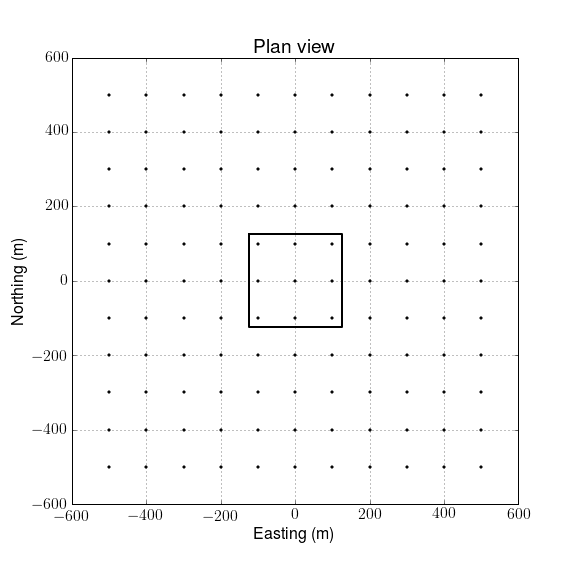
\includegraphics[width=0.5\textwidth]{figures/threecasesresp/Planview.png} \\
  (a) \\
  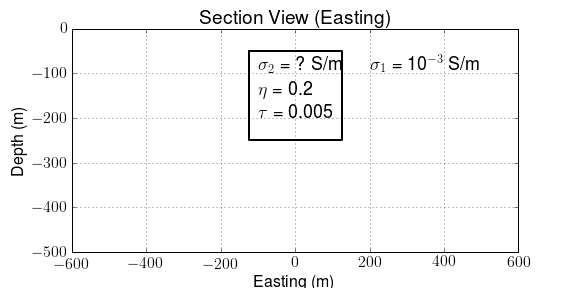
\includegraphics[width=0.5\textwidth]{figures/threecasesresp/Sectionview.png} \\
  (b)
  \caption{Plan (a) and section b) views of the IP model. Dashed line in (a) contours the boundary of the IP body. Solid circles in (a) denotes the location of stations.}
  \label{F: IPModel}
\end{figure}
\clearpage

\subsection{Analyses of ATEM-IP responses}
IP responses in ATEM data are different from different conductivity structure. Understanding different characteristics in IP response due to different conductivity can provide us important background physics. We use three different conductivity models: canonical, conductive and resistive. Then,  we proceed EM decoupling approach, which subtract $d^F$ from $d$,  assuming that we know true conductivity ($\siginf$), for all three cases and discuss features of IP response from different conductivity. 

For the coincident loop system, the most clear IP response is negative transients. Simply, we consider that our ATEM data contain IP effects when we observe negative transients. For three different cases, we start with analyzing time decaying curves at the center sounding locations (0 m easting and 0 m northing). Figure \ref{F:IPrespCurves} shows the observed ($d$), fundamental ($d^{F}$), and IP ($\dip$) responses at the center sounding location for (a) canonical, (b) conductive and (c) resistive models. We provided both $b_z$ (left panel) and $\frac{\partial b_z}{\partial t}$ (right panel). We focus on $b_z$ in following studies because of its direct connection with the IP current shown in equation (\ref{eq: BiotbIP_approx}). Polarization charge build-up may have two main phases: charging and discharging. The IP current may increase in the charging phase, and decrease in the discharging phase. This phenomenon will be proportional on $b^{IP}_z$ response thus, we choose a time when $b^{IP}_z$ has maximum amplitude with negative values. The reason behind that we only use negative values to choose reference time is based on the background that the IP current has reversed direction to the reference current (\ref{eq: jip_approx}). This moment may indicate the time when the earth has the maximum polarization charge build up. Based on this time named as the reference time ($t^{ref}$), we divide charging and discharging phases.  We first consider the canonical model ($\sigma_2 = \sigma_1$) shown in Figure \ref{F:IPrespCurves}a. In the observed data ($d$), we do not have any negative transients. However, due to the IP effect, the observed data shows rapid decay on late time channel after 1 ms. $\dip$ responses computed by the subtraction of $d^F$ from $d$, have negative sign for all times, and the reference time is $~$0.1 ms. Even at this time, $d^{F}$ is far greater than $\dip$ thus, EM induction is dominant. However, at late time after 1 ms, magnitude of $\dip$ response is considerable to that of $d^{F}$. $\frac{\partial b^{IP}_z}{\partial t}$ response show sign reversal from positive to negative at the reference time.

Second case has more conductive IP body than the background ($\sigma_2 = 10^{2}\sigma_1$). As shown in Figure \ref{F:IPrespCurves}b, we observe negative transients after $~$1 ms. Compared to canonical model, fundamental response has greater amplitude in whole time range. The maximum amplitude of $d^{F}$ is about $10^{1}$ times greater than canonical case.  In addition, $\dip$ response is greater than that of canonical case. The maximum $\dip$ is about $10^{3}$ times greater than canonical case.  The reference time occur at earlier time ($~$0.05ms) than canonical case ($~$0.1 ms), and the gradients of $\dip$ on charging and discharging are much greater than canonical case. Similar to canonical case, $\frac{\partial b^{IP}_z}{\partial t}$ response show sign reversal at the reference time. 

Third and last case is more resistive IP body than the background ($\sigma_2 = 10^{-2}\sigma_1$). Similar to the canonical case, the observed data does not have any negative values. The amplitude of the fundamental response is almost same as the canonical case. However, $\dip$ response show different phenomenon from the previous cases. $\dip$ has positive values at early time ($~$0.01 ms), and shows sign reversal at $~$0.1ms. The maximum amplitude of negative $\dip$ occurs at $~$0.4 ms. For the resistive case, there might be another level of complexity that we need to investigate based on the positive $\dip$ response at early time. We will clarify this phenomenon later by investigating the IP currents in the earth. 

While analysis of time decaying curves at one sounding location provided time behaviour of ATEM-IP response, this does not provide the geometric features of IP anomaly from all sounding locations. In order to investigate the geometric features of $\dip$ response, we show maps of $d$, $d^F$ and $\dip$ responses at early and late times from all sounding locations.  Date type here is $b_z$ (nT). Left ($d$), middle ($d^F$) and right ($\dip$) panels of Figure \ref{F:IPresp1}a shows maps for canonical model at the early time when $t=$0.03 ms. Because the canonical model does not have any conductivity contrast, $\d$ and $d^F$ at this early time does not show any anomalous response. Although $\dip$ response exists in the observed data, relative strength of $\dip$ to $d^F$ is much smaller. Figure \ref{F:IPresp1}b show three responses for conductive case. Due to  induced vortex current, which increases total current, in the the conductive body, we can observe higher anomaly both on $d$ and $d^F$ at this early time. Compared to canonical case, $\dip$ map for conductive case shows more compact distribution. Figure \ref{F:IPresp1}c show three responses for resistive case. Due to the galvanic current, which reduces total current, both $d$ and $d^{F}$ have lower anomaly. This anomalous response compared to conductive case show more spreaded distribution. Different from both canonical and conductive cases, $\dip$ response for this case shows positive anomaly, which is consistent from the observation from transient curves. For all three cases at this early time, $d^F$ is much greater than $\dip$. 

For the later time when $t=$ 7.08 ms, we provided same maps in Figure \ref{F:IPresp2}. At this time $\dip$ is greater than $d^{F}$ for all three cases. Although we do not observe any negative values on both canonical and resistive cases, by the EM decoupling process we can identify IP response embedded in the observation. Anomalous $\dip$ response for both canonical and resistive cases show more spreaded distribution than conductive case. 

To summarize, the conductive case has the strongest IP signal due to the greater amplitude of $d^{F}$ compared to other cases. $b^{IP}_z$ response has minus sign for all time range except for the resistive case, and has charging and discharging phase. For the resistive case, $\dip$ shows positive values at early times. At certain late time, IP response is considerable to the fundamental one, whereas at the early time this is challenging because the fundamental response is dominant. Therefore, an effective time range for EM decoupling can be after certain late time when the IP response is considerable to the fundamental one. At the reference time when we may have maximum polarization charge build-up, $\frac{\partial b^{IP}_z}{\partial t}$ shows zero-crossing where sign reversal occurs for all three cases. $\dip$ response from conductive case show more compact distribution on map view compared to canonical and resistive cases. 

\begin{figure}[htb]
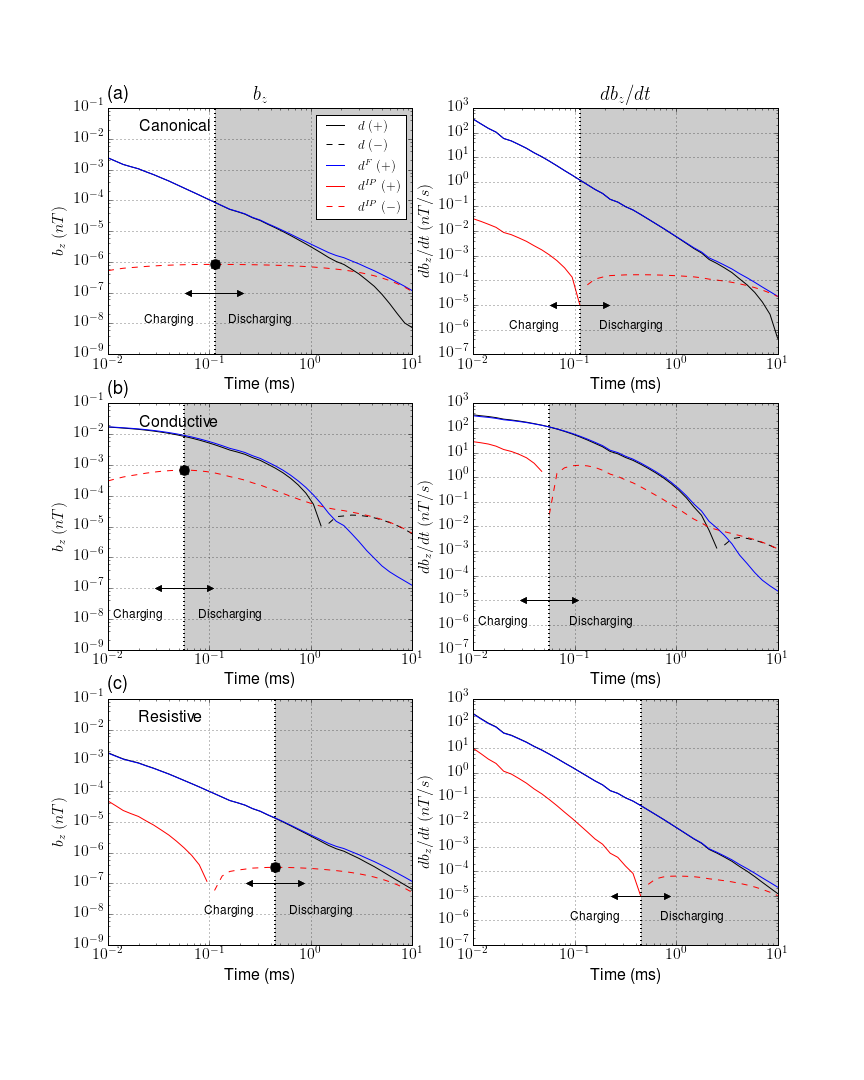
\includegraphics[width=1.0\textwidth]{figures/threecasesresp/EMIP_threecases.png}
  \centering
  \caption{Time decaying curves of $d$ (black line), $d^F$ (blue line) and $\dip$ (red line) responses for three cases: (a) canonical, (b) conductive and (c) resistive. Right and left panels show $b_z$ and $\frac{\partial b_z}{\partial t}$. }
  \label{F:IPrespCurves}
\end{figure}


\begin{figure}[htb]
  \centering  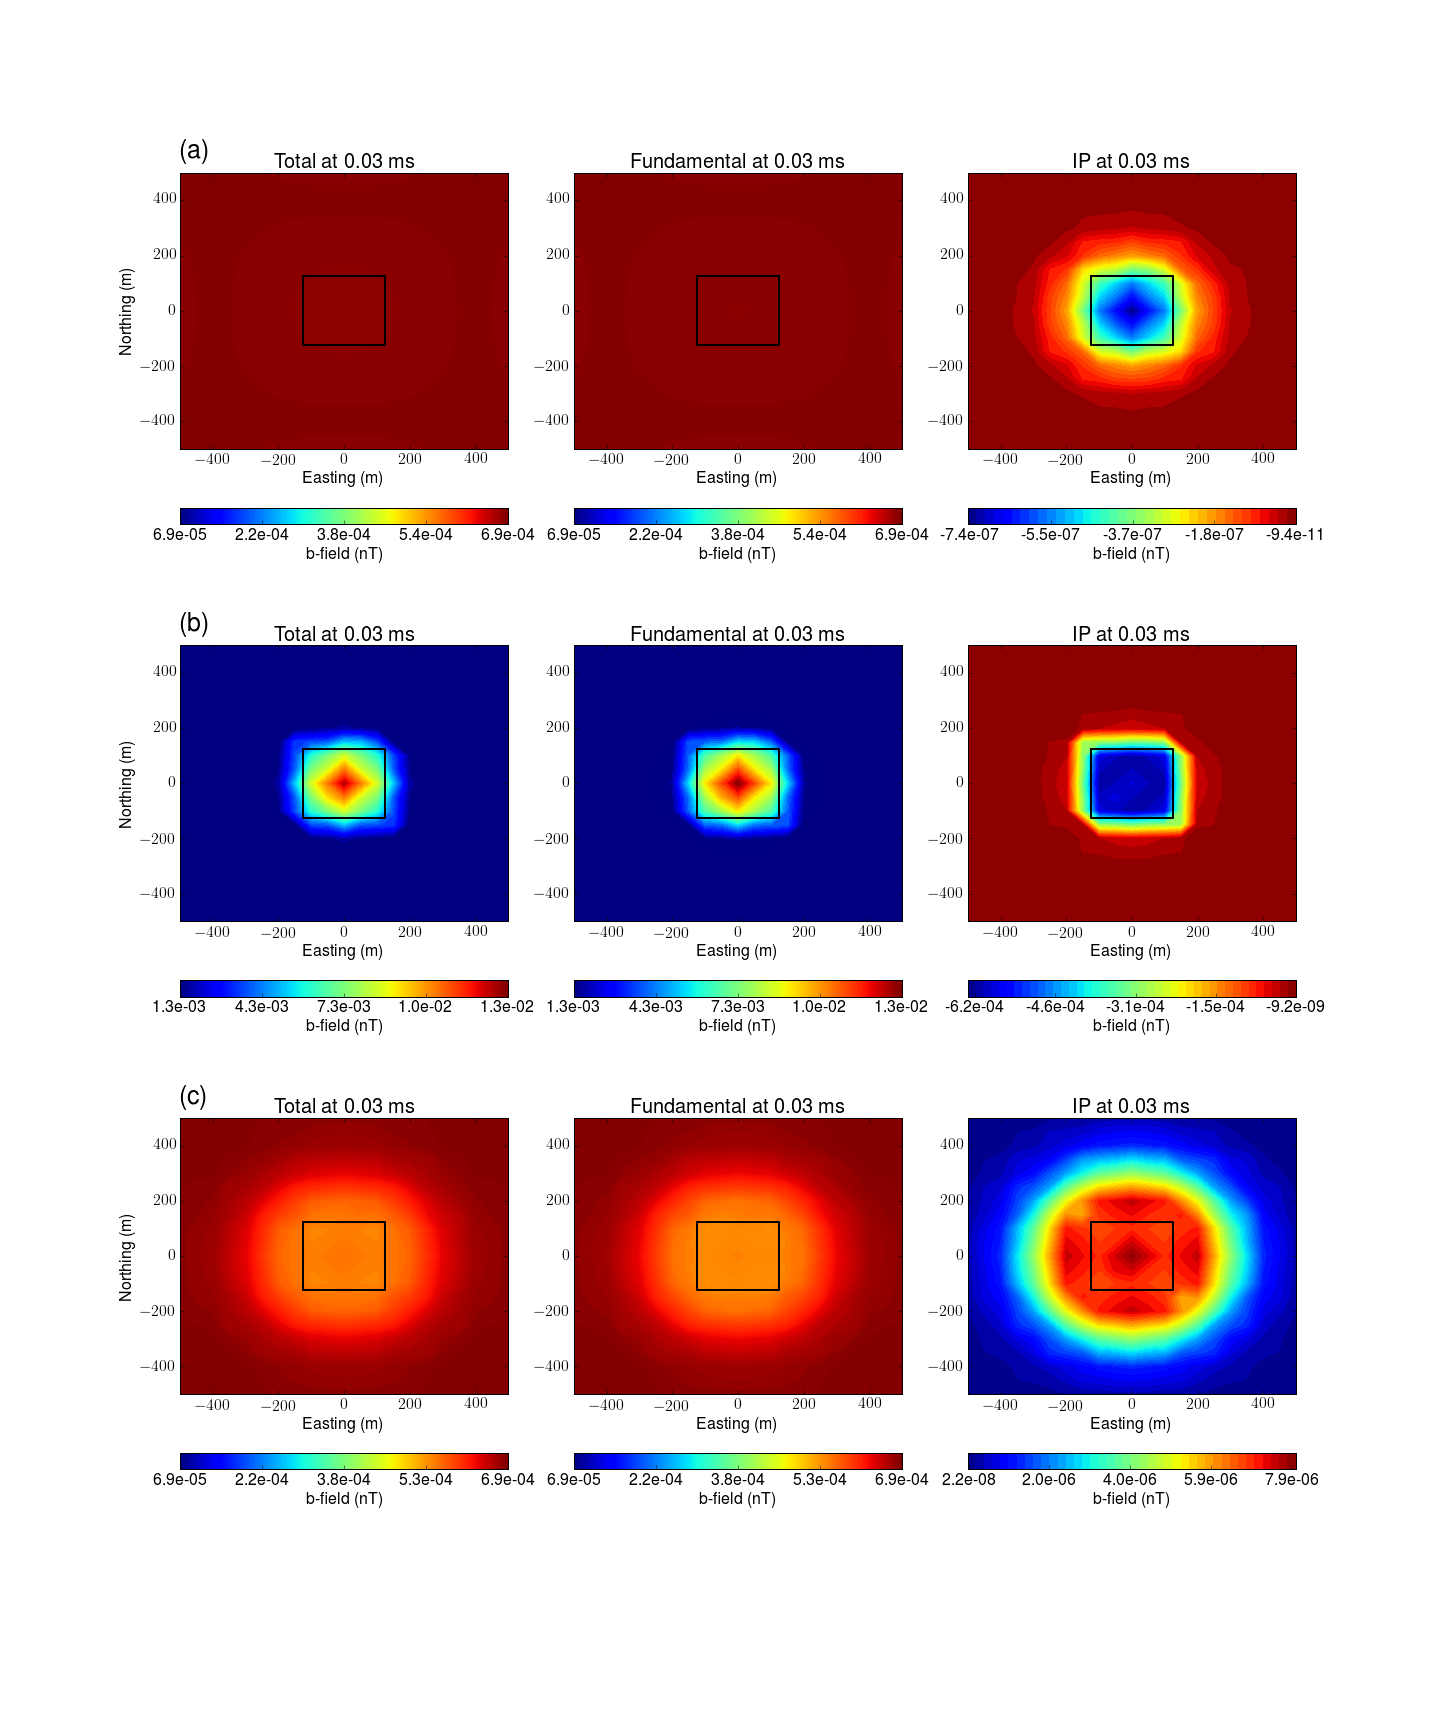
\includegraphics[width=1.0\textwidth]{figures/threecasesresp/IPresp_ch6.png}
  \caption{Response map of $d$ (left panel), $d^{F}$ (middle panel) and $\dip$ (right panel) at early time. Three maps for  (a) Canonical, (b) conductive and (c) resistive cases are shown at 0.03 ms.}
  \label{F:IPresp1}
\end{figure}

\begin{figure}[htb]
  \centering  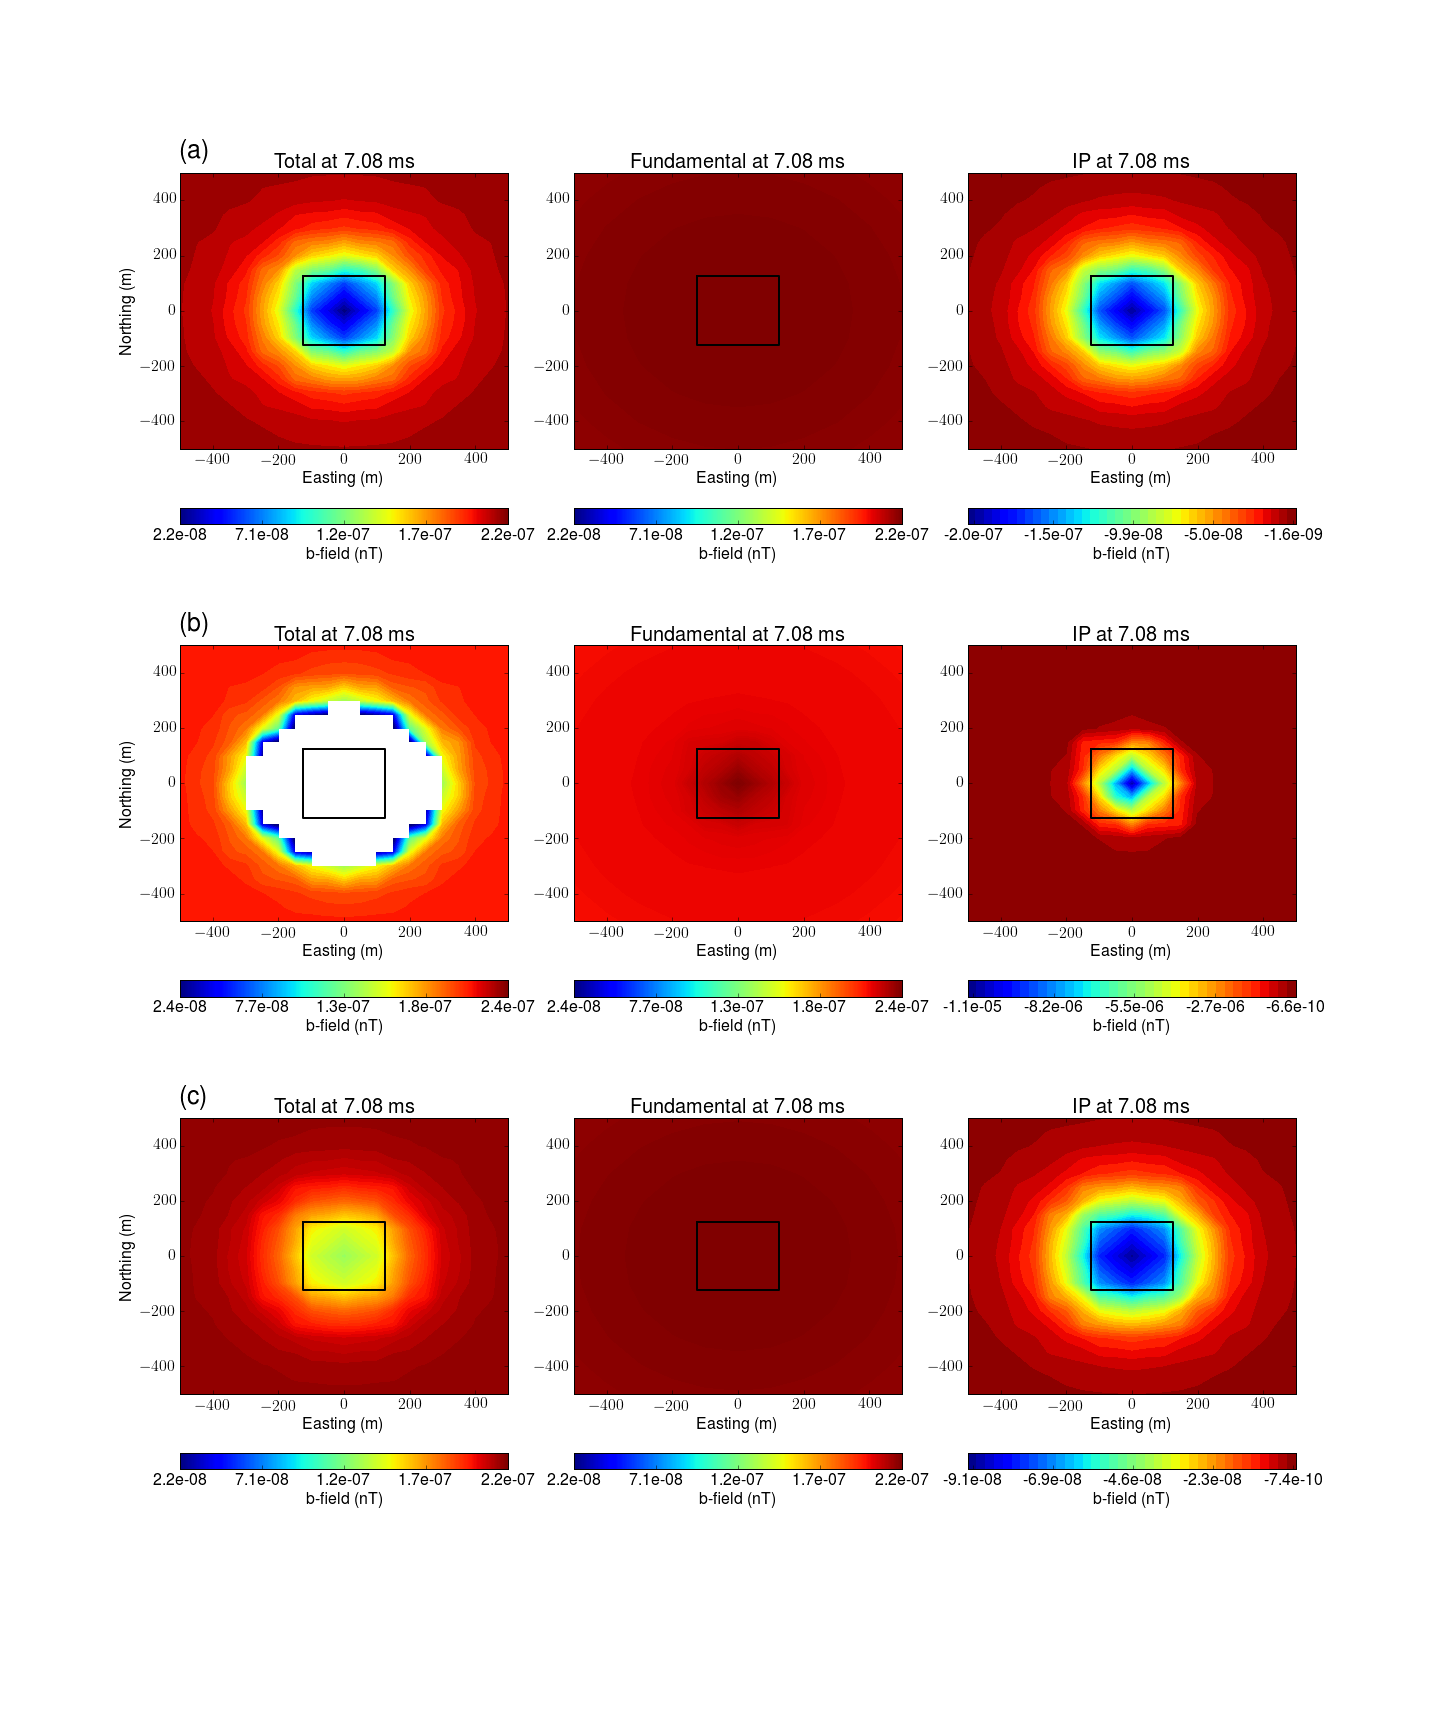
\includegraphics[width=1.0\textwidth]{figures/threecasesresp/IPresp_ch38.png}
  \caption{Response map of $d$ (left panel), $d^{F}$ (middle panel) and $\dip$ (right panel) at early time. Three maps for  (a) Canonical, (b) conductive and (c) resistive cases are shown at 7.08 ms.}
  \label{F:IPresp2}
\end{figure}
\clearpage

%Seog commenti: This mainly because galvanic current is the main source of the IP effects for both canonical and resistive cases, while for conductive case vortex current is the main source of the IP effect. 

%% =======================================================================
%% SUBSECTION
%% =======================================================================
\subsection{Analyses of IP currents}
In previous section, we analyzed the IP responses for the three different conductivity models: canonical, conductive and resistive. Although we systematically analyzed IP response for each case, investigation of the IP currents in the earth can provide us more in-depth understanding of the IP phenomenon. In addition, we had one remainig question from the previous section: $\dip$ response for the resistive case has positive values at early time. This question possibly be related to different types of IP currents: galvanic (charge build-up) and vortex (EM induction) currents. Because these two currents have different geometric shape, we can easily recognize each effect by observing the IP current in the earth. Both currents will generate magnetic field at receiver locations. We investigate total, fundamental and IP currents where transmitter loop is located at (0 m, -200 m, 30 m). 

Figure \ref{F:IPcurrents1} shows plan view maps of total (left panel), fundamental (middle panel) and IP (right panel) currents at the early time (0.03 ms).  Those currents for three different cases: (a) canonical, (b) conductive and (c) resistive are shown. From the equation (\ref{eq: jip_approx}), we can expect that the amplitude of the IP current may proportional to that of the reference currents. Direction of the IP current may be opposite to fundamental currents. Because the canonical case does not have conductivity contrast, the direction of the reference current may be similar to the fundamental current for all times. We can recognzie this expectation on three currents for the canonical case

From the geometric shape of the IP current, we recognize that the major effect of the IP current for this case is due to galvanic IP. For conductive case, we observe more localized fundamental current distribution in the conductive body. Vortex current generated in the conductive body has the same direction to fundamental current thus, this induced current increases total current.  The IP current for this case show more compact distribution in the conductive IP body than canonical case, whereas the direction of the IP currents for both cases is similar at least have opposite directions to the fundamental currents. Similarly, the galvanic IP effect is dominant in conductive case. Different from the conductive case, the fundamental current for the resistive case show reduced amplitude due to the resistive body. Furthemore, the IP current has higher amplitude outside of the body, and the direction of the IP current has the opposite directions from those of the canonical and conductive cases. Especially near the transmitter location, which is outside of the body, we recognize the vortex IP current in the direction of the fundamental current thus, the IP current increases the total current. This observation shows the reason why we have positive IP response for the resistive case at the early time. For the resistive case, both galvanic and vortex IP currents has considerable amplitude. At this early time, IP currents for all three cases show two common features: a) amplitude of the IP current is much less than the fundamental current. b) galvanic IP effect is dominant in the IP current. 

Figure \ref{F:IPcurrents2}, show the same three currents on plan view maps, but at the late time (7.08 ms). For all three cases, at this late time, the IP currents are dominant compared to the fundamental currents. Here, we recognize natural separation of EM and IP effects in time: EM effect is dominant in the early time, but decays faster than IP effect.  Thus, we observe dominant IP effect at certain late time. Considering this, we recognize the effective time range of EM decoupling will be when the relative strength of IP effect is considerable to EM effect. Although it depends upon the conductivity structure and IP parameters of the earth, but this may commonly happen at certain late time channels in practice. Geometric shape of IP currents for canonical model did not change significantly, whereas that of the amplitude decays considerably. In addition, the galvanic IP effect is dominant even at this late time. This shows the similarity with EIP case because the geometric  shape of the IP current will not change for EIP case, although it decays in time. In contrast, the IP current for the conductive case show different characteristic. Different from the early time, in the body, we observe dominant vortex IP current in late time. The IP current for conductive case has much localized distribution compared to the IP current for canonical one. Geometric shape of the IP current for the resistive case at this late time significantly changed. Even the direction of the IP current at this late time is opposite to that at the early time. This clearly shows the sign reversal in the IP responses for this case. Similar to the early time both galvanic and vortex IP current has considerable magnitudes. In contrast, the amplitude of the IP current in the body is much smaller than that in the outside of the body, whereas the canonical and conductive case has higher amplitude in the body. 

In summary, due to the natural separation of the EM and IP effects in time we can expect considerable IP effect in certain late time, and this is the time when we have some possibilities to recognize IP responses embedded in the observation. For the canonical model, the galvanic IP effect is the main driving force of the IP current. The IP current for the conductive case shows transition from galvanic to vortex currents as time increases. Both galvanic and vortex IP currents has considerable amplitude for the resistive case. Conductive case show the strongest amplitude of the IP current. Geometric shape of the IP currents for canonical case does not change significantly from early to late time, whereas those for the conductive and resistive cases show considerable changes in time. 

\begin{figure}[htb]
  \centering  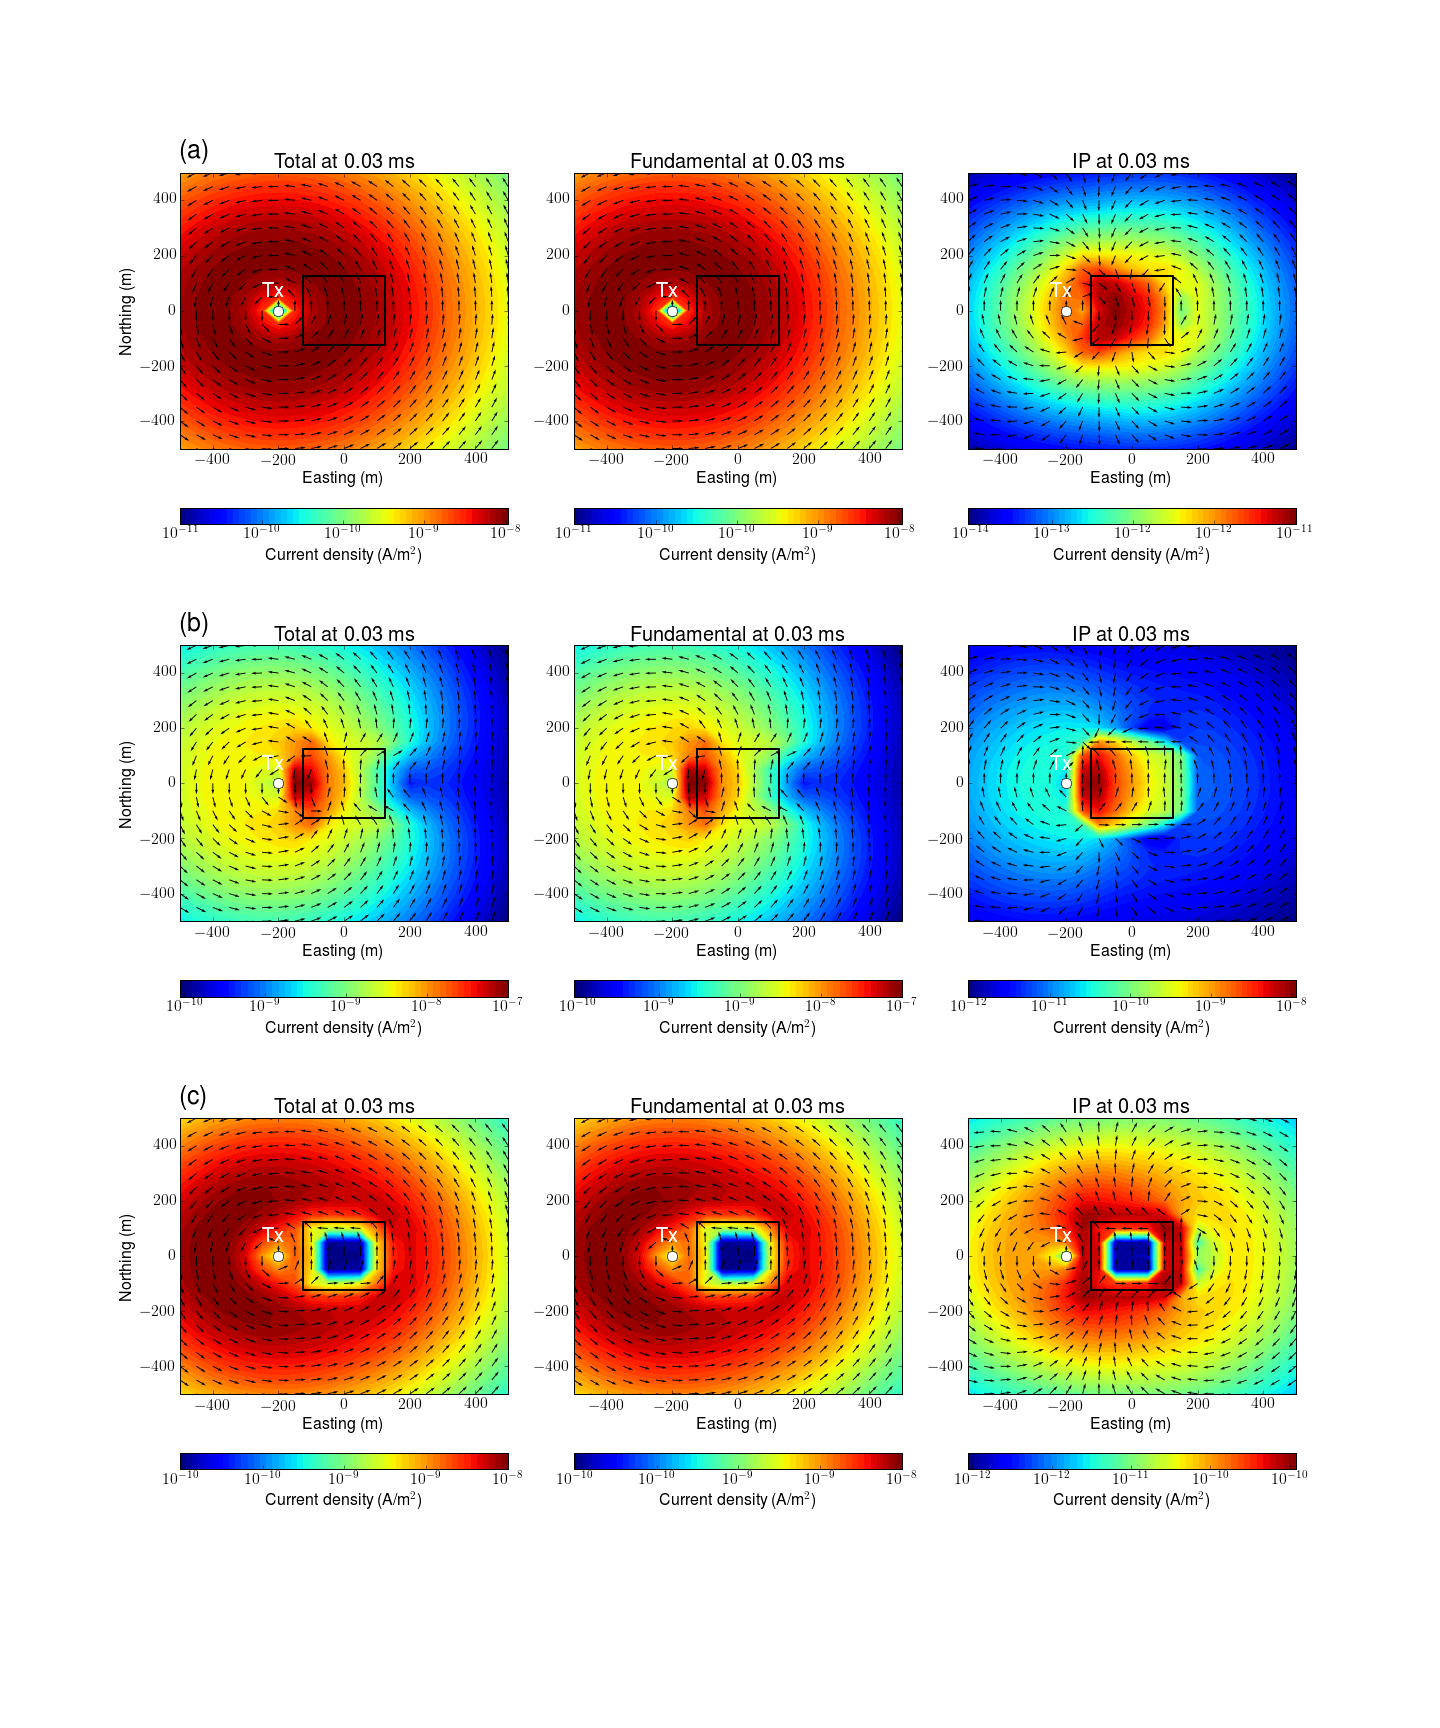
\includegraphics[width=1.0\textwidth]{figures/threecasesresp/IPcurrents_ch6.png}
  \caption{Maps of total, fundamental and IP currents at early time. Three maps for  (a) Canonical, (b) conductive and (c) resistive cases are shown at 7.08 ms.}
  \label{F:IPcurrents1}
\end{figure}
\begin{figure}[htb]
  \centering  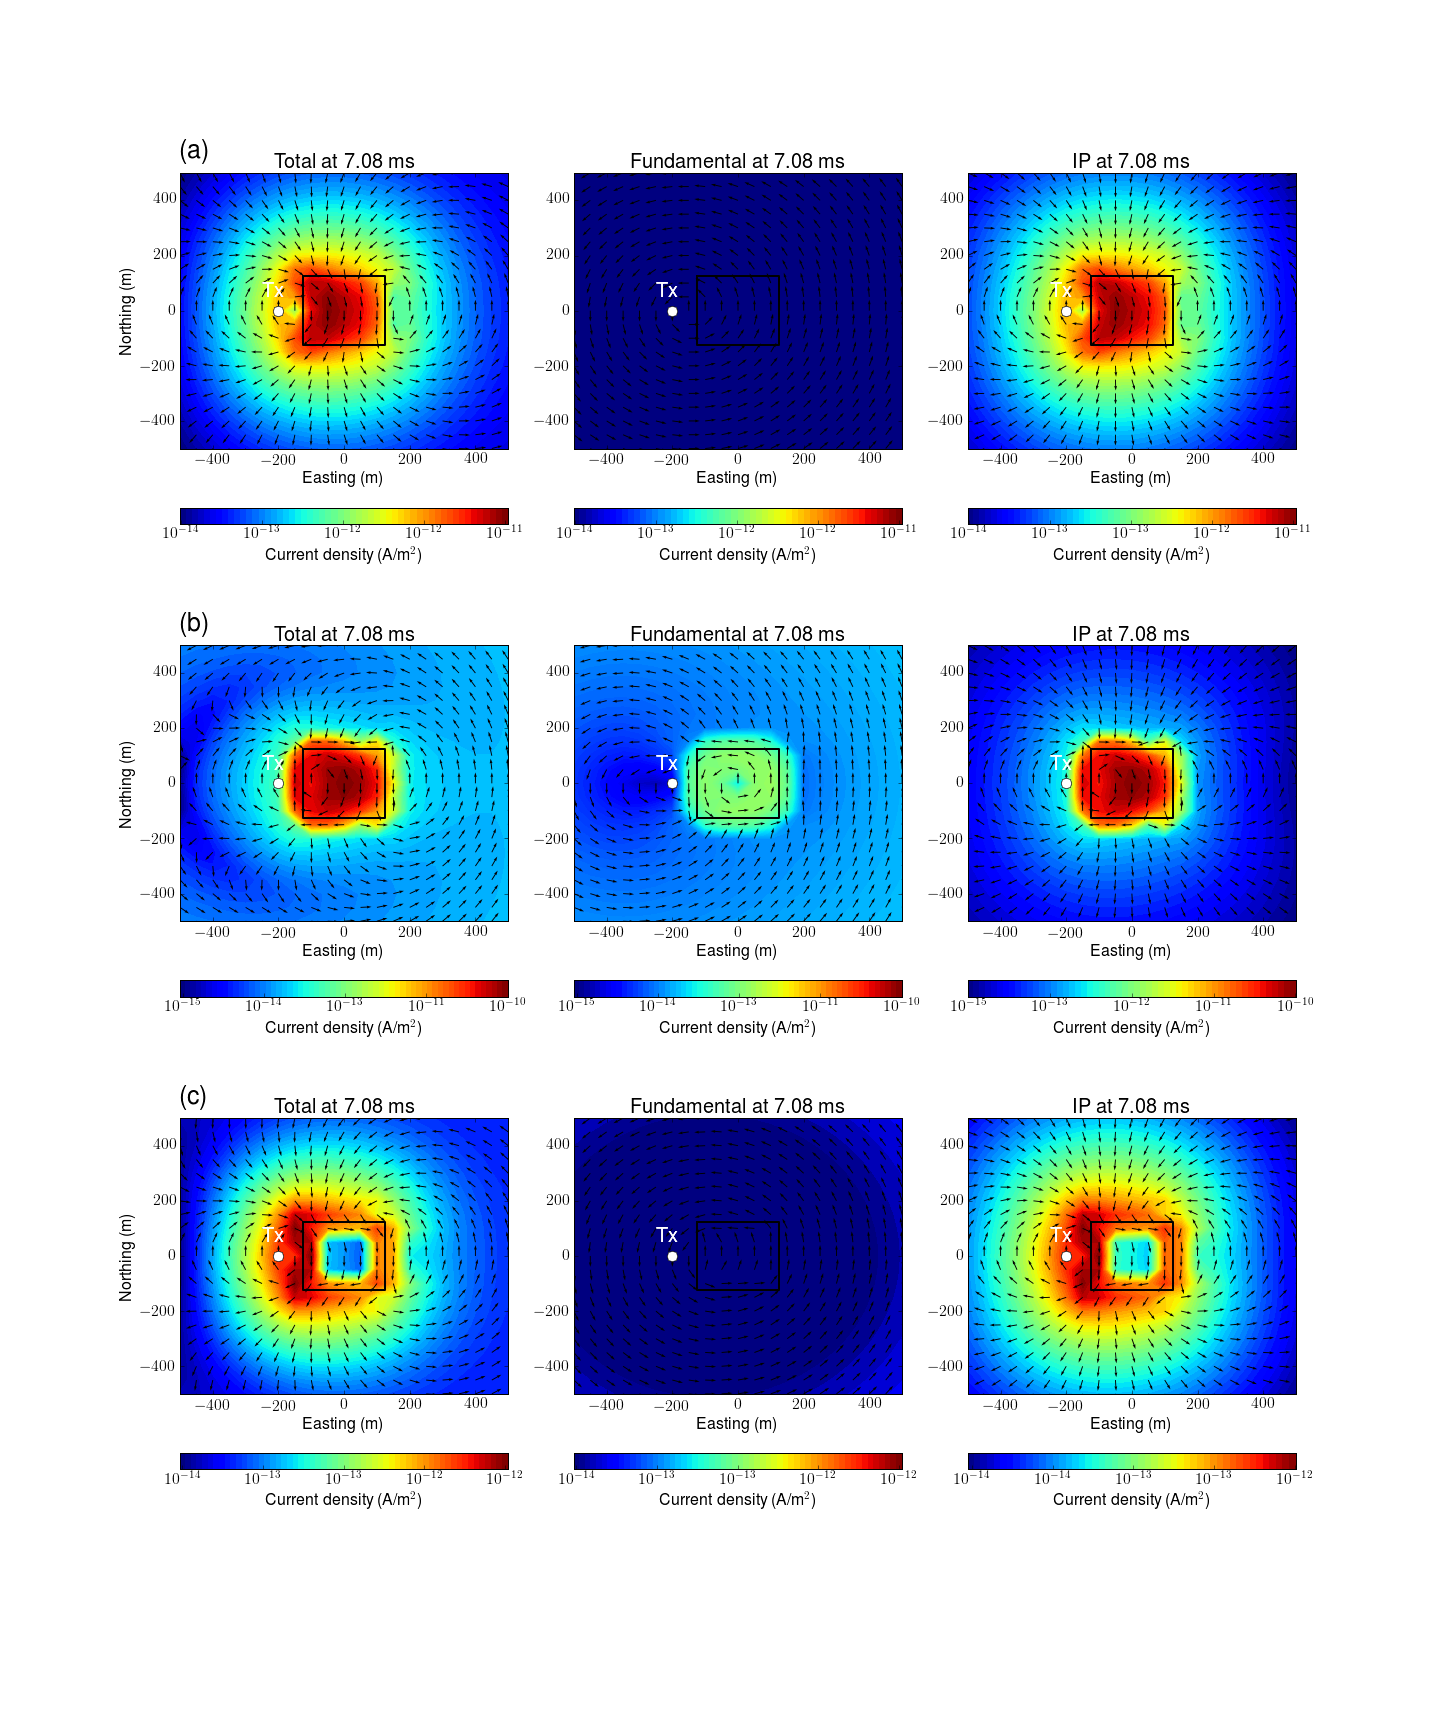
\includegraphics[width=1.0\textwidth]{figures/threecasesresp/IPcurrents_ch38.png}
  \caption{Maps of total, fundamental and IP currents at early time. Three maps for  (a) Canonical, (b) conductive and (c) resistive cases are shown at 7.08 ms.}
  \label{F:IPcurrents2}
\end{figure}

%% =======================================================================
%% SUBSECTION
%% =======================================================================
\subsection{Validation of linearization}

%% =======================================================================
%% SUBSUBSECTION
\subsubsection{IP current}
To obtain a linearized kernel in equations (\ref{eq: BiotbIP_approx}), we approximate the IP current as a function of the pseudo-chargeability. Then by using Biot-Savart law, we evaluate $\dip$ response at the receiver location. To show the applicability of our approximate solution, we compare both the IP current and $\dip$ response for the approximate solution with those for the true one. We use the same three conductivity structures to investigate these comparisons. To compute the linearized kernel function, we need to choose the time when the amplitude of fundamental current reaches to the maximum for each pixel in 3D. This time and the current were called the maximum time ($t^{max}$) and current ($\j^{F}_{max}$). For all three conductivity models, we computed these $\j^{F}_{max}$ and $t^{max}$ (Figure \ref{F:jmaxtmax}). The maximum current for canonical case show vortex current, which is centered at the transmitter location. The maximum time for this case increases as the horizontal distance from the transmitter location increases. This makes sense because a closer pixel from the transmitter location will reach the maximum before a farther pixel does. Due to the conductivity contrasts in conductive and resistive models, $\j^{F}_{max}$ and $t^{max}$ show different features from those for the canonical case. The maximum current for the conductive cases shows the increased amplitude near the transmitter location. In addition, we observe the vortex current in the conductive body due to the induced vortex current in the history of time. This is clearly shown in $t^{max}$: in the body, the current reaches to the maximum on later time. In contrast, for the resistive case, the amplitude of $\j^{F}_{max}$ is decreased both near the transmitter and in the body. Because of its resistive nature, the current reaches to the maximum time at earlier time in the body. Considering the assumption we made for the polarization current: $\j^{pol}(t) = -\j^F_{max}\peta(t)$, we can recognize that the effect of different conductivity structure in the IP current can be captured through $\j^{F}_{max}$. 

Using these maximum currents for each case with the equation (\ref{eq: jip_approx}), we can compute the approximate IP current ($\j^{IP}_{approx}$). We compare the true and approximate $\j^{IP}$. Figures \ref{F:jIPcomparison_early} and \ref{F:jIPcomparison_late} show the comparisons of the true and approximate IP currents on plan view maps at the early (0.03 ms) and late (7.08 ms) times, respectively.  In addition, we plotted time decaying curves of total, fundamental and those two IP currents in $y$-direction at a single pixel in the body (noted as Rx in the figures) on Figure \ref{F:jIPcomparison_decay} for canonical (a), conductive (b) and resistive (c) models. Thick dashed and solid lines indicate the early and late times used on above plan view maps. The true and approximate IP currents for the canonical case almost coincident not only on plan view maps at this late time (7.08 ms), but also on the early time as shown in Figures \ref{F:jIPcomparison_early} and \ref{F:jIPcomparison_late}. Furthermore, the time decaying curves of these IP currents are almost coincident on all times as shown in Figure \ref{F:jIPcomparison_decay}. Thus, for the canonical case, our assumptions on the IP current is reasonable for all time range. For the conductive case, at the late time, true and approximate IP currents show reasonable match, whereas they show significant difference at the early time (Middle column of Figures \ref{F:jIPcomparison_early} and \ref{F:jIPcomparison_late}). The approximate IP current for the conductive case converges to the true one near 2 ms (Figure \ref{F:jIPcomparison_decay}b) thus, our approximate solution is reasonable near this time for conductive case. Different from two previous cases, the IP current for resistive case have greater amplitude on the outside of the body. At the early time, the approximate solution show significant difference from true one. Even at the late time, the amplitude of true and approximate IP currents show considerable difference on the outside of the body. However, those for inside of the body show reasonable match. In addition, the direction of the true and approximate IP currents are almost identical at the late time. We summarized above comparisons in Figure (\ref{F:tableIPcurrent}). A principal assumption that we made for the polarization current was $\j^{pol}(t) \approx \j^{F}_{max}\peta(t)$. The observation that the approximate IP current in the body show good approximation for all three cases at late time suggests that the above approximation is reasonable after a certain the late time when the amplitude of the IP current is consierable to that of the fundamental current. At this late time period, the approximate IP current show good match with true one for all three cases except for the amplitude of resistive case. This makes the applicability of the linearized kernel function somewhat arguable for the resistive case. 

\begin{figure}[htb]
  \centering  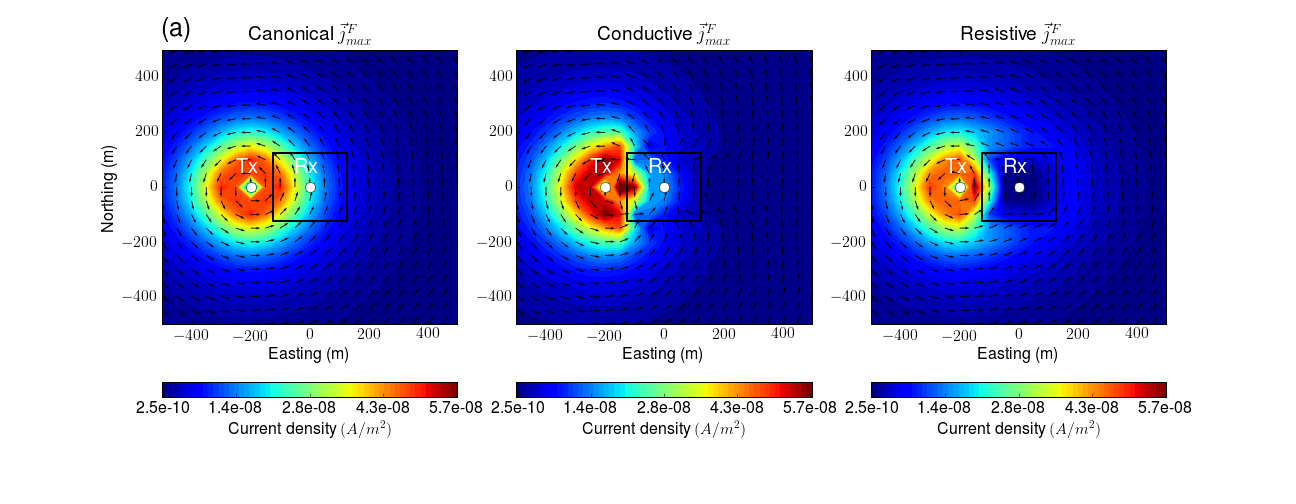
\includegraphics[width=1.0\textwidth]{figures/threecasesresp/jmax.png}\\
  \centering  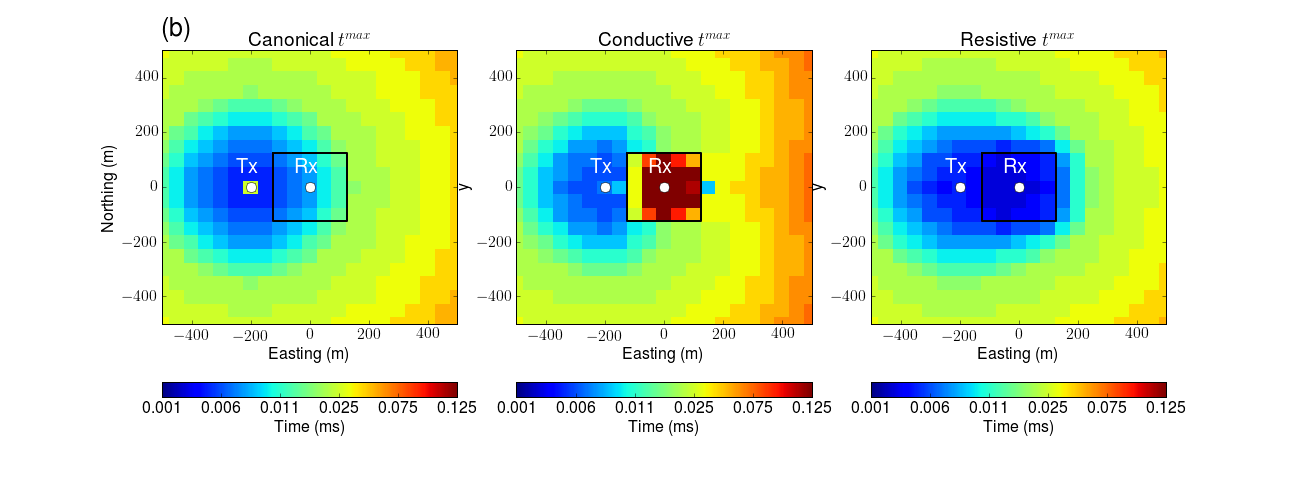
\includegraphics[width=1.0\textwidth]{figures/threecasesresp/tmax.png}
  \caption{Plan view maps of $\j^{F}_{max}$ (a) and $t^{max}$ (b) at -125 m depth. Left, middle and right panels correspondingly show those for canonical, conductive and resistive models.}
  \label{F:jmaxtmax}
\end{figure}

\begin{figure}[htb]
\centering  
    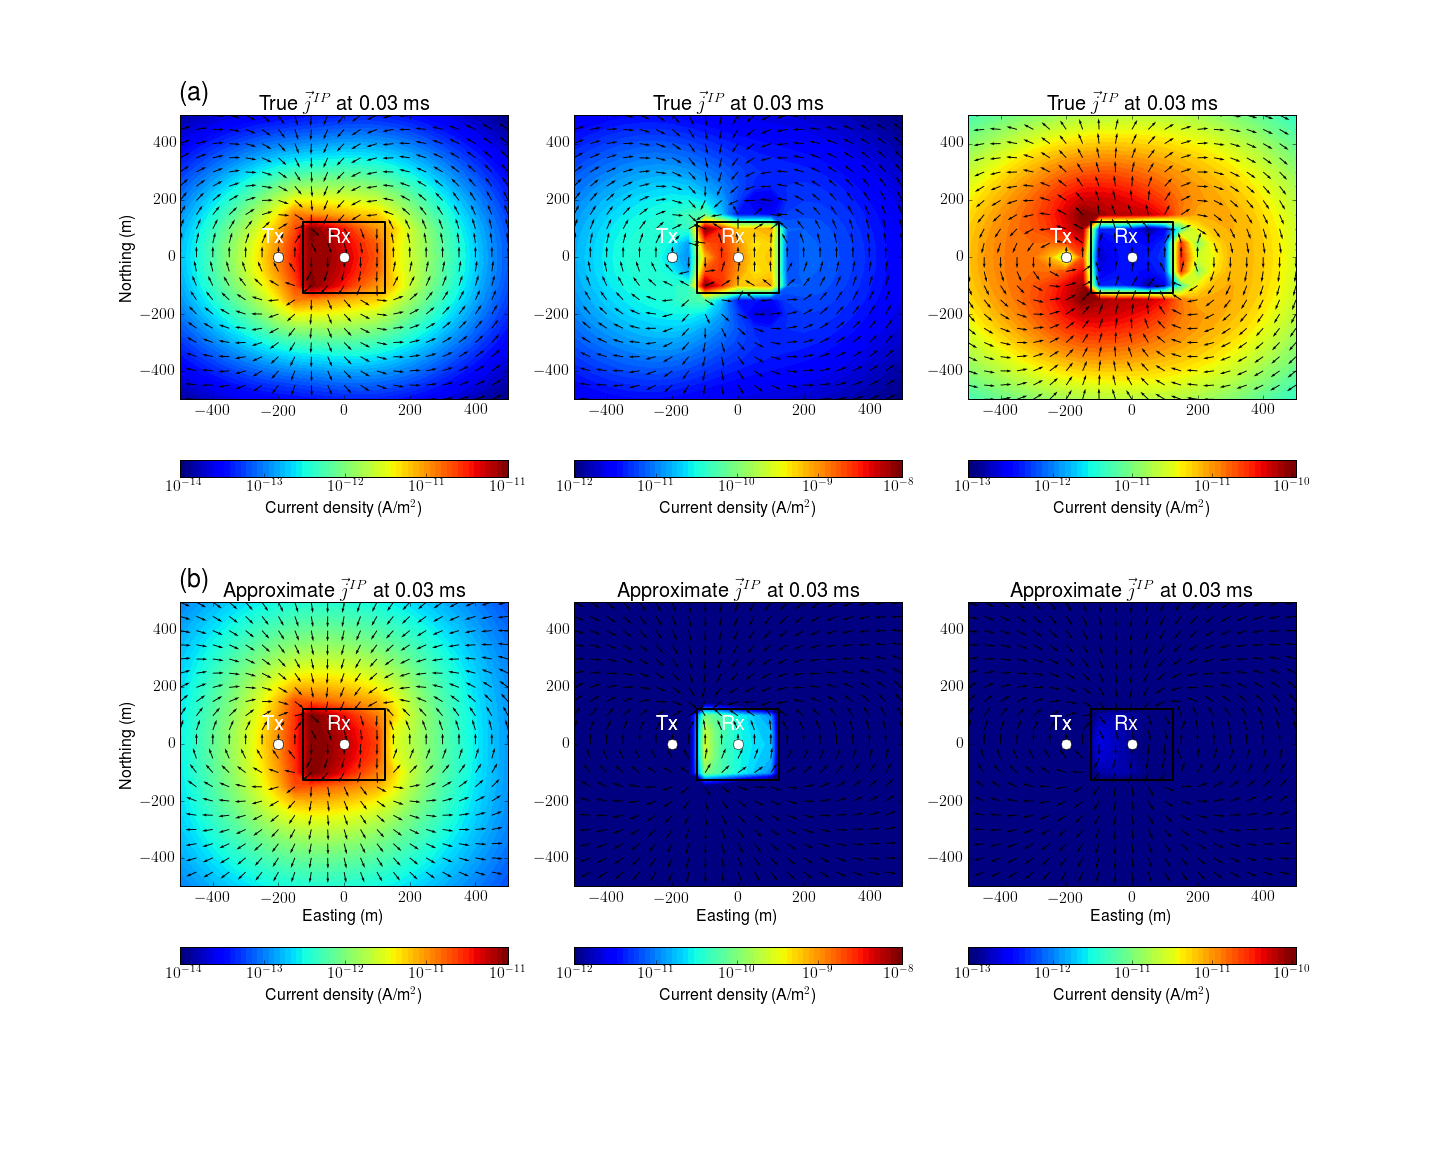
\includegraphics[width=1.0\textwidth]{figures/threecasesresp/jIPcomparison_ch6.png}
    \caption{Plan view maps of the true (a) and approximate (b) $\j^{IP}$ at -125 m depth and t=0.03 ms. Left, middle and right panels correspondingly show those for canonical, conductive and resistive models.}
  \label{F:jIPcomparison_early}
\end{figure}

\begin{figure}[htb]
  \centering  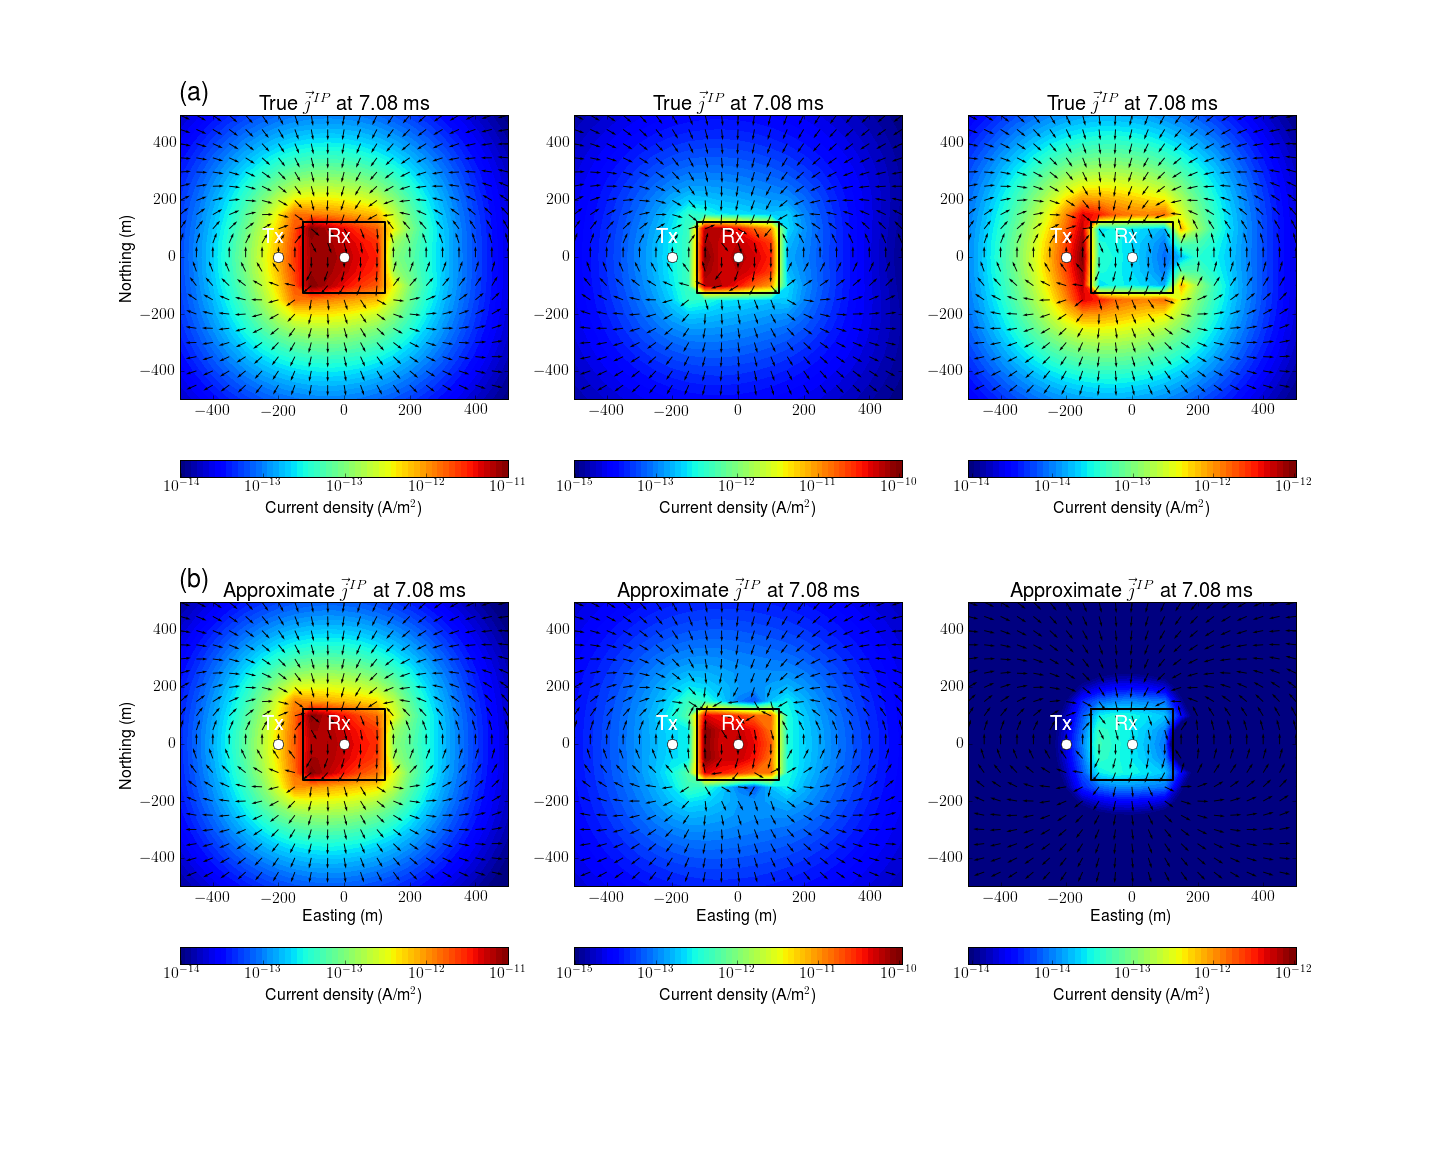
\includegraphics[width=1.0\textwidth]{figures/threecasesresp/jIPcomparison_ch38.png}
  \caption{Plan view maps of the true (a) and approximate (b) $\j^{IP}$ at -125 m depth and t=7.08 ms. Left, middle and right panels correspondingly show those for canonical, conductive and resistive models.}
  \label{F:jIPcomparison_late}
\end{figure}


\begin{figure}[htb]
  \centering  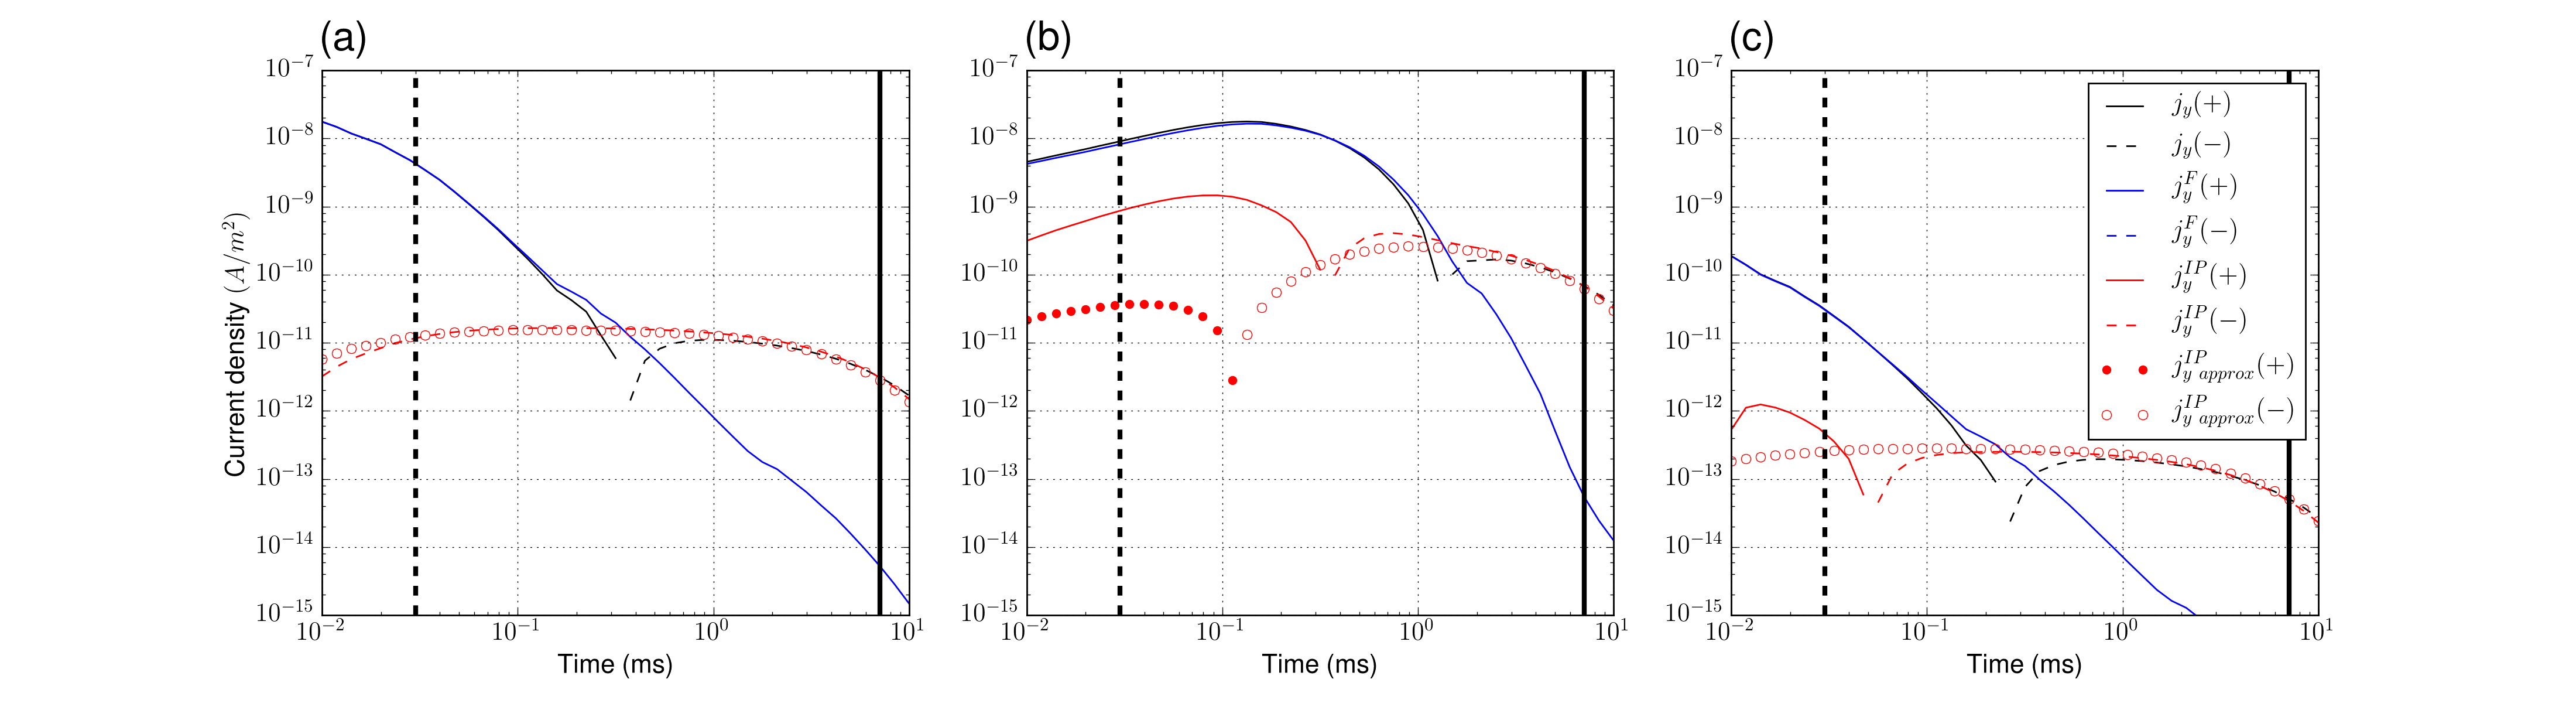
\includegraphics[width=1.0\textwidth]{figures/threecasesresp/jIPcomparison_decay.png}\\
  \caption{Plan view maps of the true (a) and approximate (b) $\j^{IP}$ at -125 m depth. Left, middle and right panels correspondingly show those for canonical, conductive and resistive models.}
  \label{F:jIPcomparison_decay}
\end{figure}

\begin{figure}[htb]
  \centering  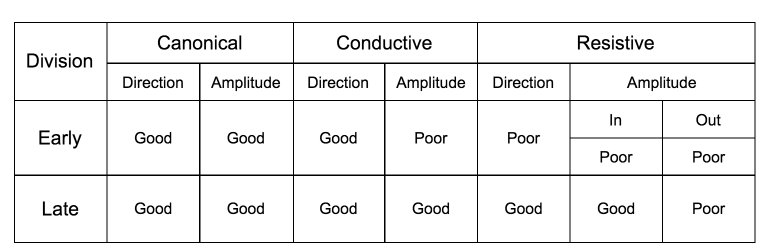
\includegraphics[width=1.0\textwidth]{figures/threecasesresp/tableIPcurrent.png}
  \caption{Comparisons of the applicability of the approximate IP currents for three different cases: canonical, conductive and resistive conductivity models. }
  \label{F:tableIPcurrent}
\end{figure}

\clearpage

%% =======================================================================
%% SUBSUBSECTION
\subsubsection{IP response}
Although the IP current is the core of the linearized kernel function, the output of this function is $\dip$ response, which was evaluated by using Biot-Savart law with the approximate IP current. In order to validate the linearized kernel, we also need to compare $\dip$ response generated by the linearized kernel function with the true $\dip$ response, which is computed by subtraction process shown in equation (\ref{eq: IPdatum_syn}). Because we use the coincident loop system the receiver location is same as the transmitter location. The data type we chose in our example is a vertical component of magnetic flux density ($b^{IP}_z$). To show the reliability of applying Biot-Savart law, we also plotted $b^{IP}_z$ response computed by using Biot-Savart law ($b^{IP}_{z \ BS}$) with the true IP current. As shown in Figure \ref{F:compIPresp}, they are almost identical to true $b^{IP}_z$. In the same figure, we compare the true and approximate $\dip$ responses for three cases. The true and approximate IP responses for the canonical model (black) shows good match on all times except for very early time ($~$0.01 ms). The approximate IP response for the conductive case (blue)  converges to the true one as we go to the later time, whereas they show significant difference on early time. This is consistent result with the phenomenon on the approximate IP current of the conductive case. The true and approximate IP responses for the resistive case show considerable difference for all times due to the poor amplitude of the approximate IP current. 

\begin{figure}[htb]
  \centering  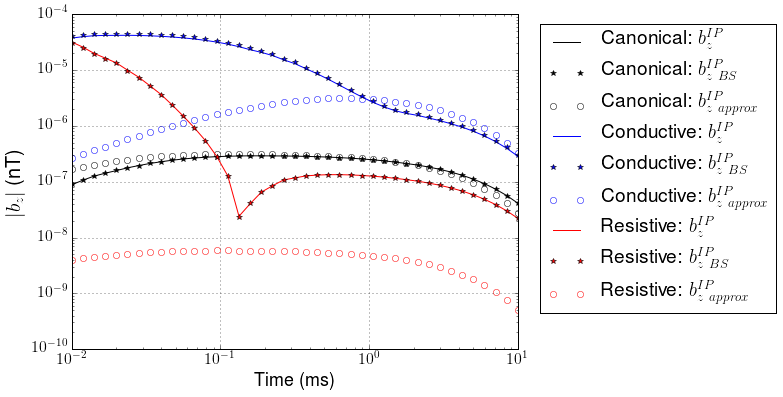
\includegraphics[width=1.0\textwidth]{figures/threecasesresp/compIPresp.png}
  \caption{Comparison of of true and approximate $\dip$ responses. The data type here is vertical component of the magnetic flux density ($b_z$). Black, blue and red color correspondingly stand for canonical, conductive and resistive cases. }
  \label{F:compIPresp}
\end{figure}
\clearpage

%% =======================================================================
%% SUBSUBSECTION
\subsubsection{Discussion for the resistive case}
Comparisons of the true and approximate solutions for the IP current and response suggest that our linearized kernel function is reasonable at certain late time except for the resistive case. This is mostly resulted from the poor approximation for the amplitude of the IP current. Then why the approximate IP current lose the amplitude? We try to explain this phenomenon by decomposing the IP current as three parts:
\begin{equation}
  \j^{IP} = \j^{pol} -\vec{a}^{IP}_J-\grad \phi^{IP}_J, 
\end{equation}
where $\siginf\e^{IP} = -\vec{a}^{IP}_J - \grad \phi^{IP}_J$. This is Helmholtz decomposition of $\siginf\e^{IP}$ thus, $\div \vec{a}^{IP}_J = 0$. Because we recognized that our approximation for  $\j^{pol}$ is good, a possible source of the reason why our assumption show poor performance for the resistive case, is $\siginf \e^{IP}$. In addition, considering Biot-savart law shown in equation (\ref{eq: Biot}), computed $\b^{IP}$ does not affected by $\grad \phi^{IP}_J$ because it is curl-free component. Therefore, if the relative strength of $\vec{a}^{IP}_J$ is greater than $\j^{pol}$, the approximate IP current may not describe the amplitude of the true IP current and this will induce same effect on the approximate $\dip$ response. Figure \ref{F:jpolvsj1IP} show $\j^{pol}$, $-\vec{a}^{IP}_J$ and $-\grad \phi^{IP}_J$ for all three cases at 7.08 ms. The amplitude of the polarization current for canonical and conductive cases at this late time are greater than those of  $\vec{a}^{IP}_J$ and $\grad \phi^{IP}_J$. However, in the resistive case, the amplitude of $\vec{a}^{IP}_J$ is greater than that of $\j^{pol}$. This shows the reason why our approximation has poor description for the amplitude of the true IP current and $\dip$ response in the resistive case. 

\begin{figure}[htb]
  \centering  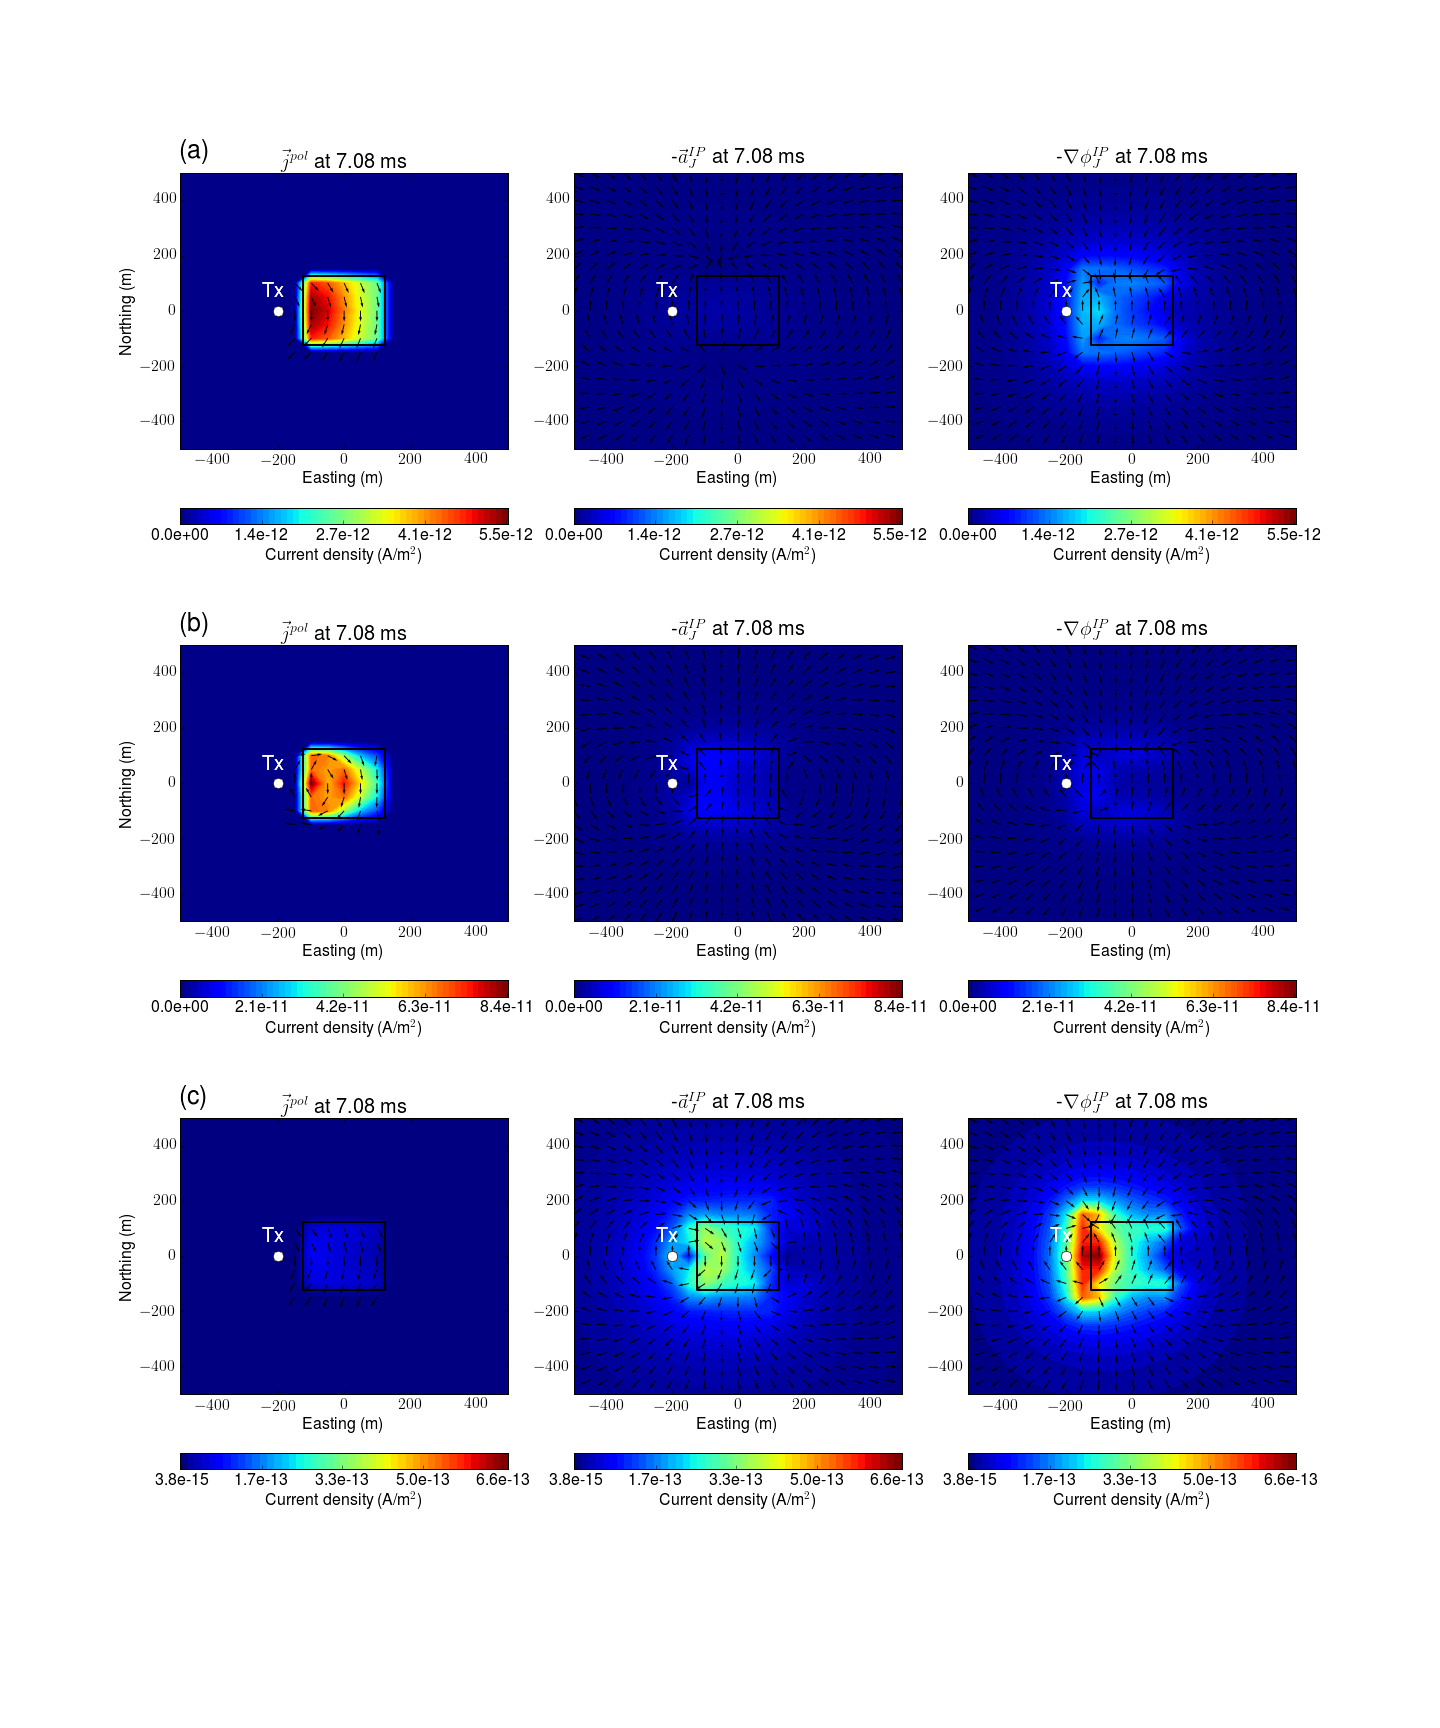
\includegraphics[width=1.0\textwidth]{figures/threecasesresp/jpolvsj1IP_ch38.png}
  \caption{Plan view maps of the true (a) and approximate (b) $\j^{IP}$ at -125 m depth and t=7.08 ms. Left, middle and right panels correspondingly show those for canonical, conductive and resistive models.}
  \label{F:jpolvsj1IP}
\end{figure}
\clearpage

%% =======================================================================
%% SUBSUBSECTION
\subsection{A potential for recovering IP parameters}

Although the physical understanding of the linearized kernel function is important, our final goal will be the IP inversion of the ATEM data. To investigate a potential of this task, we extract intrinsic IP parameters from a single pixel of the pseudo-chargeability, which is located at the center of the IP body (marked as Rx on Figures \ref{F:jIPcomparison_late}). Recalling that the pseudo-chargeability is the convolution between $\peta^{I}(t)$ and $w^{e}(t)$ (\ref{eq: pseudochargeability}), we need to solve a deconvolution problem to extract intrinsic IP parameters including $\eta$ and $\tau$. Since we consider Debye case ($c=1$) for Cole-Cole model, we assume that we know $c$. Definition of the intrinsic pseudo-chargeability is shown in equation (\ref{eq: intrinsic_peta}). We compute $\peta$ and $w^e$ for all three cases to make a synthetic data for this deconvolution problem. Using a conventional deconvolution problem, which directly recover impulse response, we can recover $\peta^{I}(t)$. However, we are more interested in Cole-Cole parameters including $\eta$ and $\tau$. Accordingly, we set these two IP parameters as our inversion model. Using the Gauss-Newton method, we optimize this problem and recover these two parameters. We consider the pseudo-chargeability at a single pixel as the observed data, and convolution between $\peta^{I}(t)$ and $w^e(t)$ as a forward problem. Figure \ref{F:wepetathree}a and b show $w^e(t)$ and comparisons of the observed and predicted data. Because $w^e(t)$ can be considered as the normalized time history of the electric field, for all cases it starts from zero and increases until it reaches to the peak.  After that it decays. Resistive case reaches to the maximum at the earliest time. Canonical and conductive cases reach at the maximum almost same time, although the conductive case show much slower decay after this time. Those phenomenon make sense considering their conductivity features in terms of the EM induction. As shown in Figure, recovered $\tau$ and $\eta$ are same as true ones, and the observed and predicted data show good matches. The true $\tau$ and $\eta$ for all three cases were 0.005 and 0.2, respectively. Considering the approximate IP currents in the body for all three cases showed good match with the true ones (Figure \ref{F:jIPcomparison_decay}), we can recognize the potential for recovering intrinsic IP parameters from airborne time domain EM data. 

\begin{figure}[htb]
  \centering  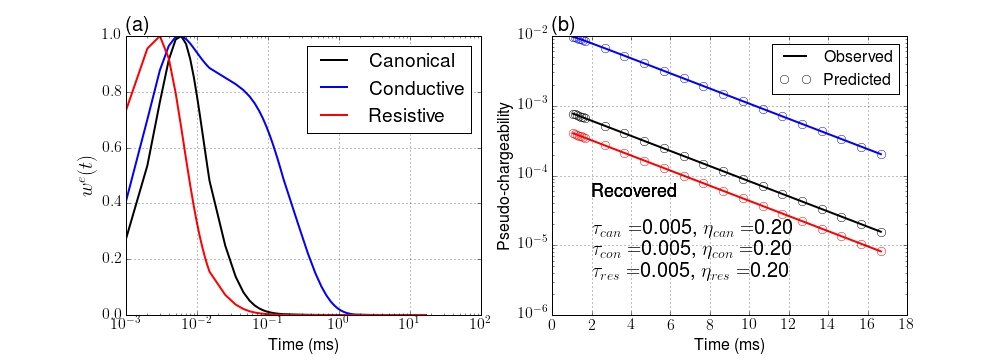
\includegraphics[width=1.0\textwidth]{figures/threecasesresp/wepetathree.png}
  \caption{(a) The normalized time history of the fundamental electric field ($w^e(t)$) for all three cases. Black, blue and red colors correspondingly indicate canonical, conductive and resistive cases. (b) Comparisons of the observed (line) and predicted (empty circles) pseudo-chargeability at the center pixel in the IP body for three cases.}
  \label{F:wepetathree}
\end{figure}

%% =======================================================================
%% SUBSUBSECTION 

% \subsection{Linear inversion}
% We apply linear inversion to restore 3D distribution of pseudo-chargeability at each time channels. In order to validate our inversion algorithm, we first generated synthetic IP data, $\dip_{syn}$ for both canonical and conductive models using forward equation shown in equation (\ref{eq: BiotbIPdt_approx}). Floor noise of $0.01max(|\mathbf{d}^{obs}|)$ was added to $\dip_{syn}$, and we set this as our uncertainty ($\epsilon$). Here data type is $\frac{\partial b_z}{\partial t}$. We use same survey configuration that we used to compute $\dip$ responses. As shown in Table 1, the number of data for each time channel is 121, since we have 121 stations. Our model parameter do not include air, thus the number of model parameters: 41$\times$41$\times$20=33620. Since our sensitivity function has higher values near the surface, we need to balance this biased sensitivity distribution. This has been carefully treated in magnetic inversion (CITE). Based on this, we use $\mathbf{w} = (\mathbf{z}+z_0)^{-1.5}$ with $z_0$=0 for model weighting shown in equation (\ref{eq: weight_mat}). Here $\mathbf{z}$ is discretized depth for all model parameters, $z_0$ indicates the depth of the earth surface. Other inversion parameters are shown in Table 1. A constant, related to initial $\beta$, $r_{\beta}$ is set to 1. To generate sensitivity matrix shown in equation (\ref{eq: dbIPdt_linear}), we used true background conductivity model for both cases. Same Cole-Cole parameters are used ($\eta$=0.2, $\tau$=0.005 and $c$=1), and for $\peta$ we used $\peta^{I}$, which was shown in equation (\ref{eq: intrinsic_peta}) when $c$=1.

% \begin{table}[ht]
% \caption{Parameters used in Projected Gauss Newton inversion.} % title of Table
% \centering % used for centering table
% \begin{tabular}{c c} % centered columns (4 columns)
% \hline\hline %inserts double horizontal lines
% Inversion parameters & Value \\
% [0.1ex] % inserts table
% \hline
% The number of data &    11$\times$11=121 \\
% The number of models &  41$\times$41$\times$20=33620 \\
% $\alpha_s$ &  $10^{-5}$\\
% $\alpha_x$ &  1\\
% $\alpha_y$ &  1\\
% $\alpha_z$ &  1\\
% Initial $\beta$ &  $r_{\beta}\frac{\mathbf{x}^T\mathbf{J}^T\mathbf{J}\mathbf{x}}{\mathbf{x}^T\mathbf{W}_m^T\mathbf{W}_m\mathbf{x}}$\\
% Decrease rate of $\beta$ &  0.5\\
% The number of $\beta$ iteration & 2\\
% $\mathbf{m}_{ref}$ & $10^{-10}$ \\
% Uncertainty & $\epsilon$=$0.01$max($|\mathbf{d}^{obs}|$) \\
% Bound constraint & $\mathbf{m} > 0$\\
% \hline %inserts single line
% \end{tabular}
% \label{table:1} % is used to refer this table in the text
% \end{table}

% Linear inversions are applied $\dip_{syn}$ data at t=4.7 ms so that corresponding $\peta^I$ value for IP body is 8.52. In Figure ~\ref{F: Peta_dipsyn_ch38}a and b, we presented inverted peudo-chargeablity models for both canonical and conductive models, respectively. To show reliability of our inversion, observed and predicted data for both canonical and conductive model were shown in Figure ~\ref{F: ObsPred_syn_ch38}a and b, respectively. Observed and predicted data for both cases show reasonable matches. Also, both inversions were reached to th target misfit. In both cases, geometry of IP body was well imaged in right location, whereas estimated $\peta$ for canonical model shows somewhat blurred image compared to that for conductive model. Recovered $\peta$ values in the IP body for both cases were $~$1.5 and $~$4.4, whereas true $\peta$ value for the IP body was 8.72. As Figure ~\ref{F: ObsPred_syn_ch38}a and b, $\dip_{syn}$ for canonical model shows broader distribution than that for conductive model, which may explain different magnitude of restored $\peta$ for both cases. These observations of recovered $\peta$ for both cases shows that recovered model from conductive model can have bigger magnitude compared to canonical model. In addition, by comparing $\dip_{syn}$ shown in the left panel of Figure ~\ref{F: ObsPred_syn_ch38}a and b with true $\dip$ data shown in the right panels of Figures ~\ref{F: EMIPresp2_case1}b and ~\ref{F: EMIPresp2_case2}b, we recognize that their geometric distribution for both cases are analogous, whereas their absolute values are different. This suggest the reliability of our linearization approach.

% \begin{figure}[htb]
%   \centering
%   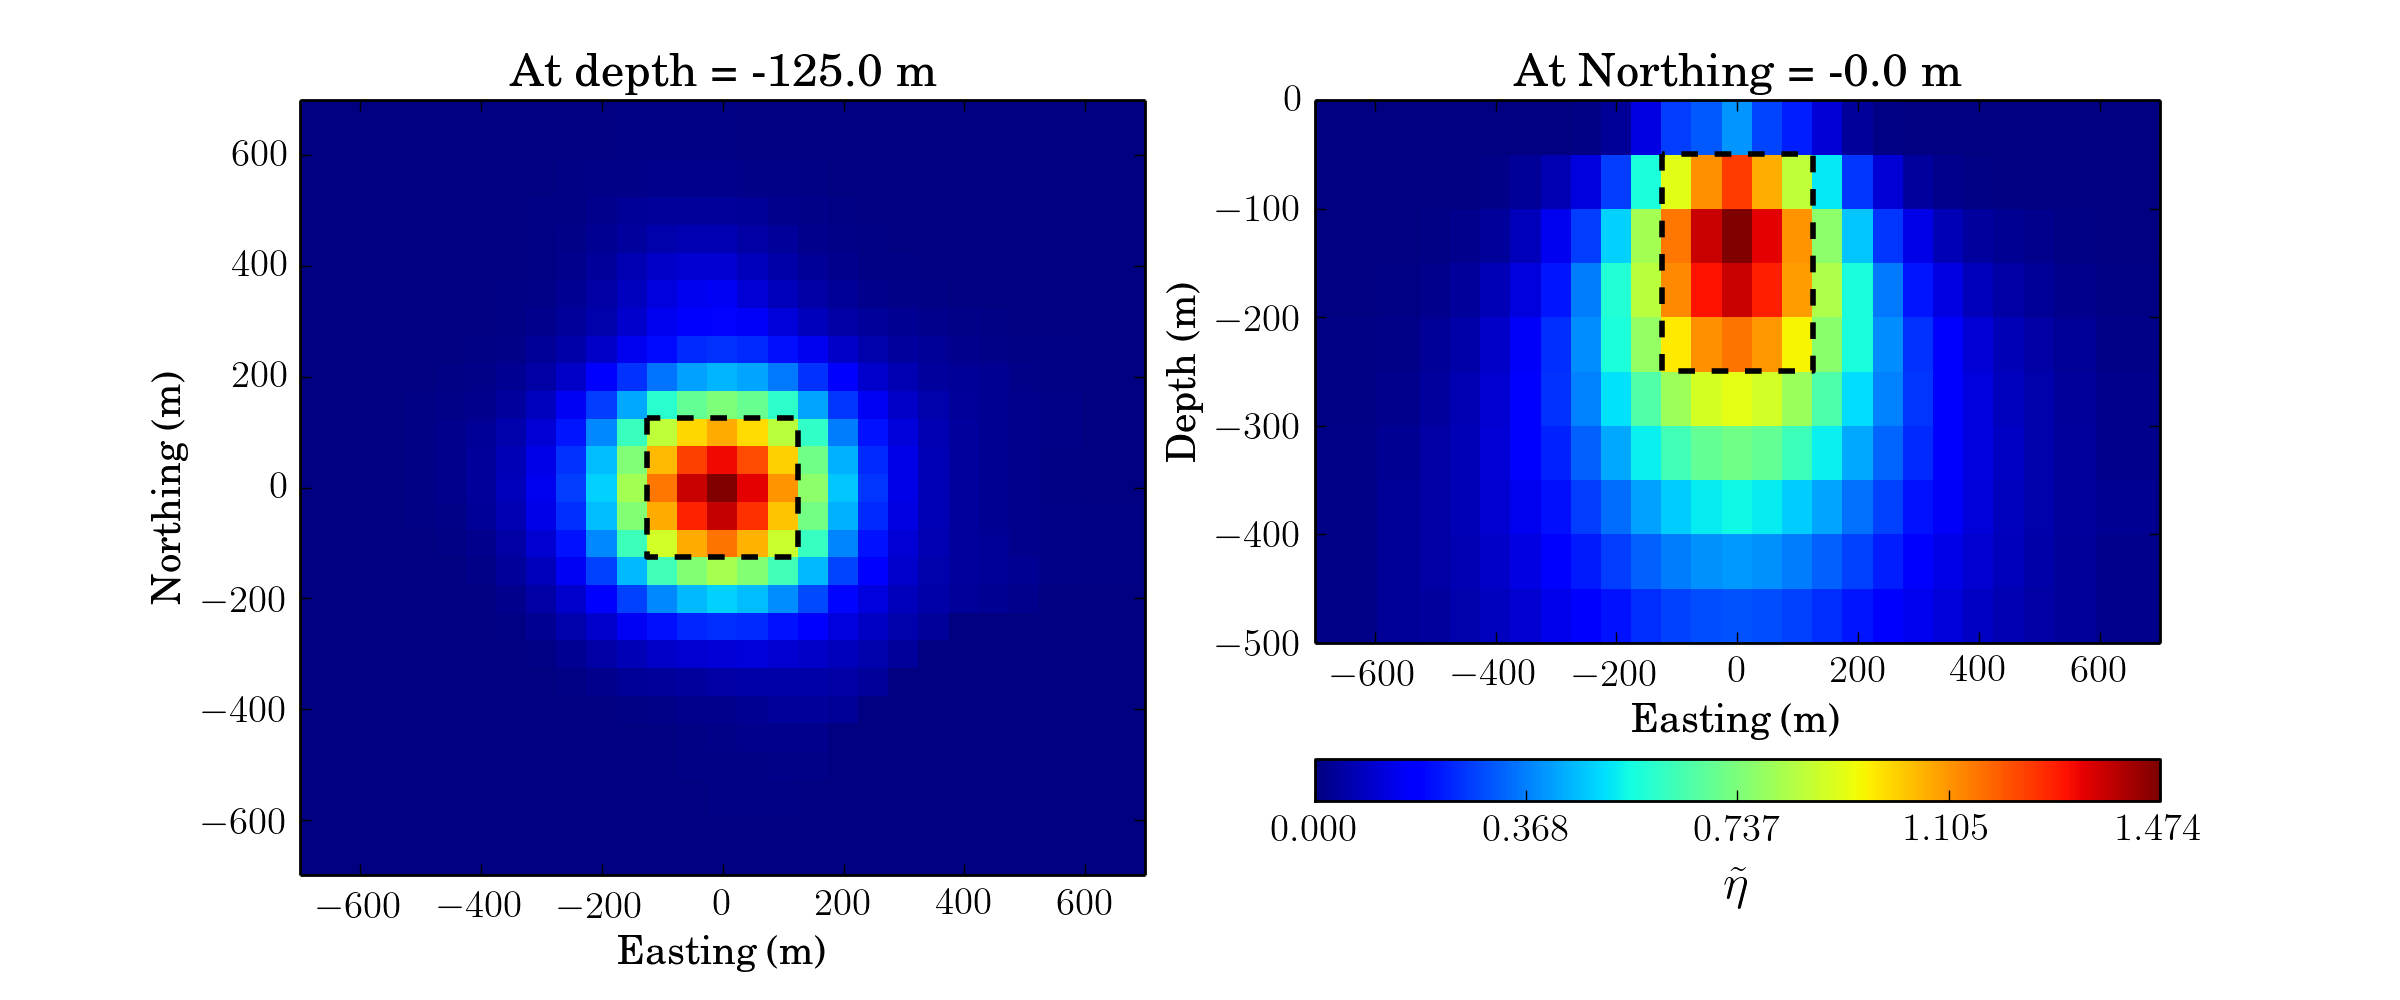
\includegraphics[width=\textwidth]{figures/synthetic/PetaCase1_syn_ch38.png}\\
%   (a)
%   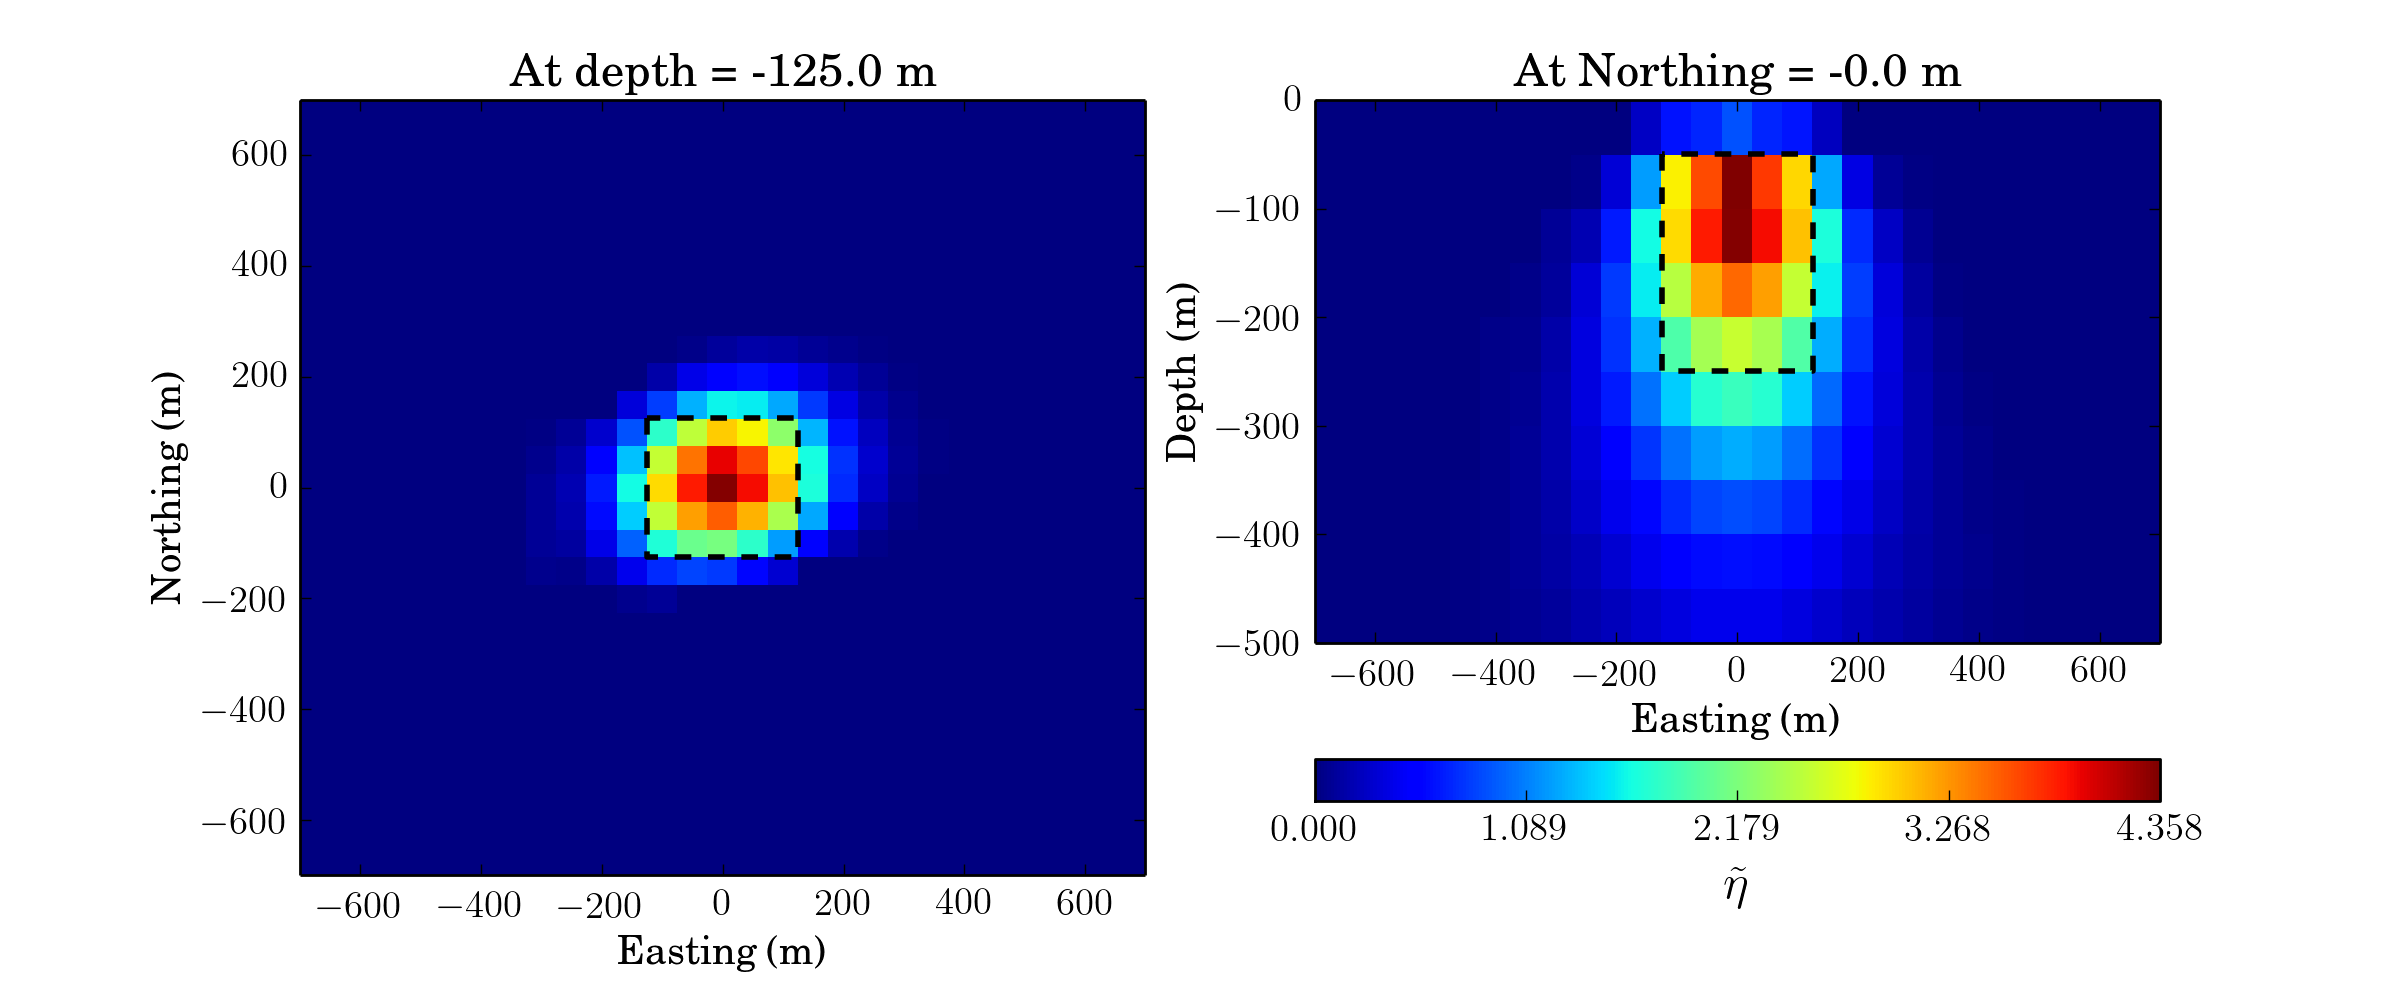
\includegraphics[width=\textwidth]{figures/synthetic/PetaCase2_syn_ch38.png}\\
%   (b)
%   \caption{Slices of estimated $\peta$ distributions at $t = $ 4.7 ms by inverting $\dip_{syn}$. (a) Canonical model. (b)  Conductive model. Left and right panel show plan and section view at -125 m depth and 0 m northing. Black dashed lines outline IP body. }
%   \label{F: Peta_dipsyn_ch38}
% \end{figure}

% \begin{figure}[htb]
%   \centering
%   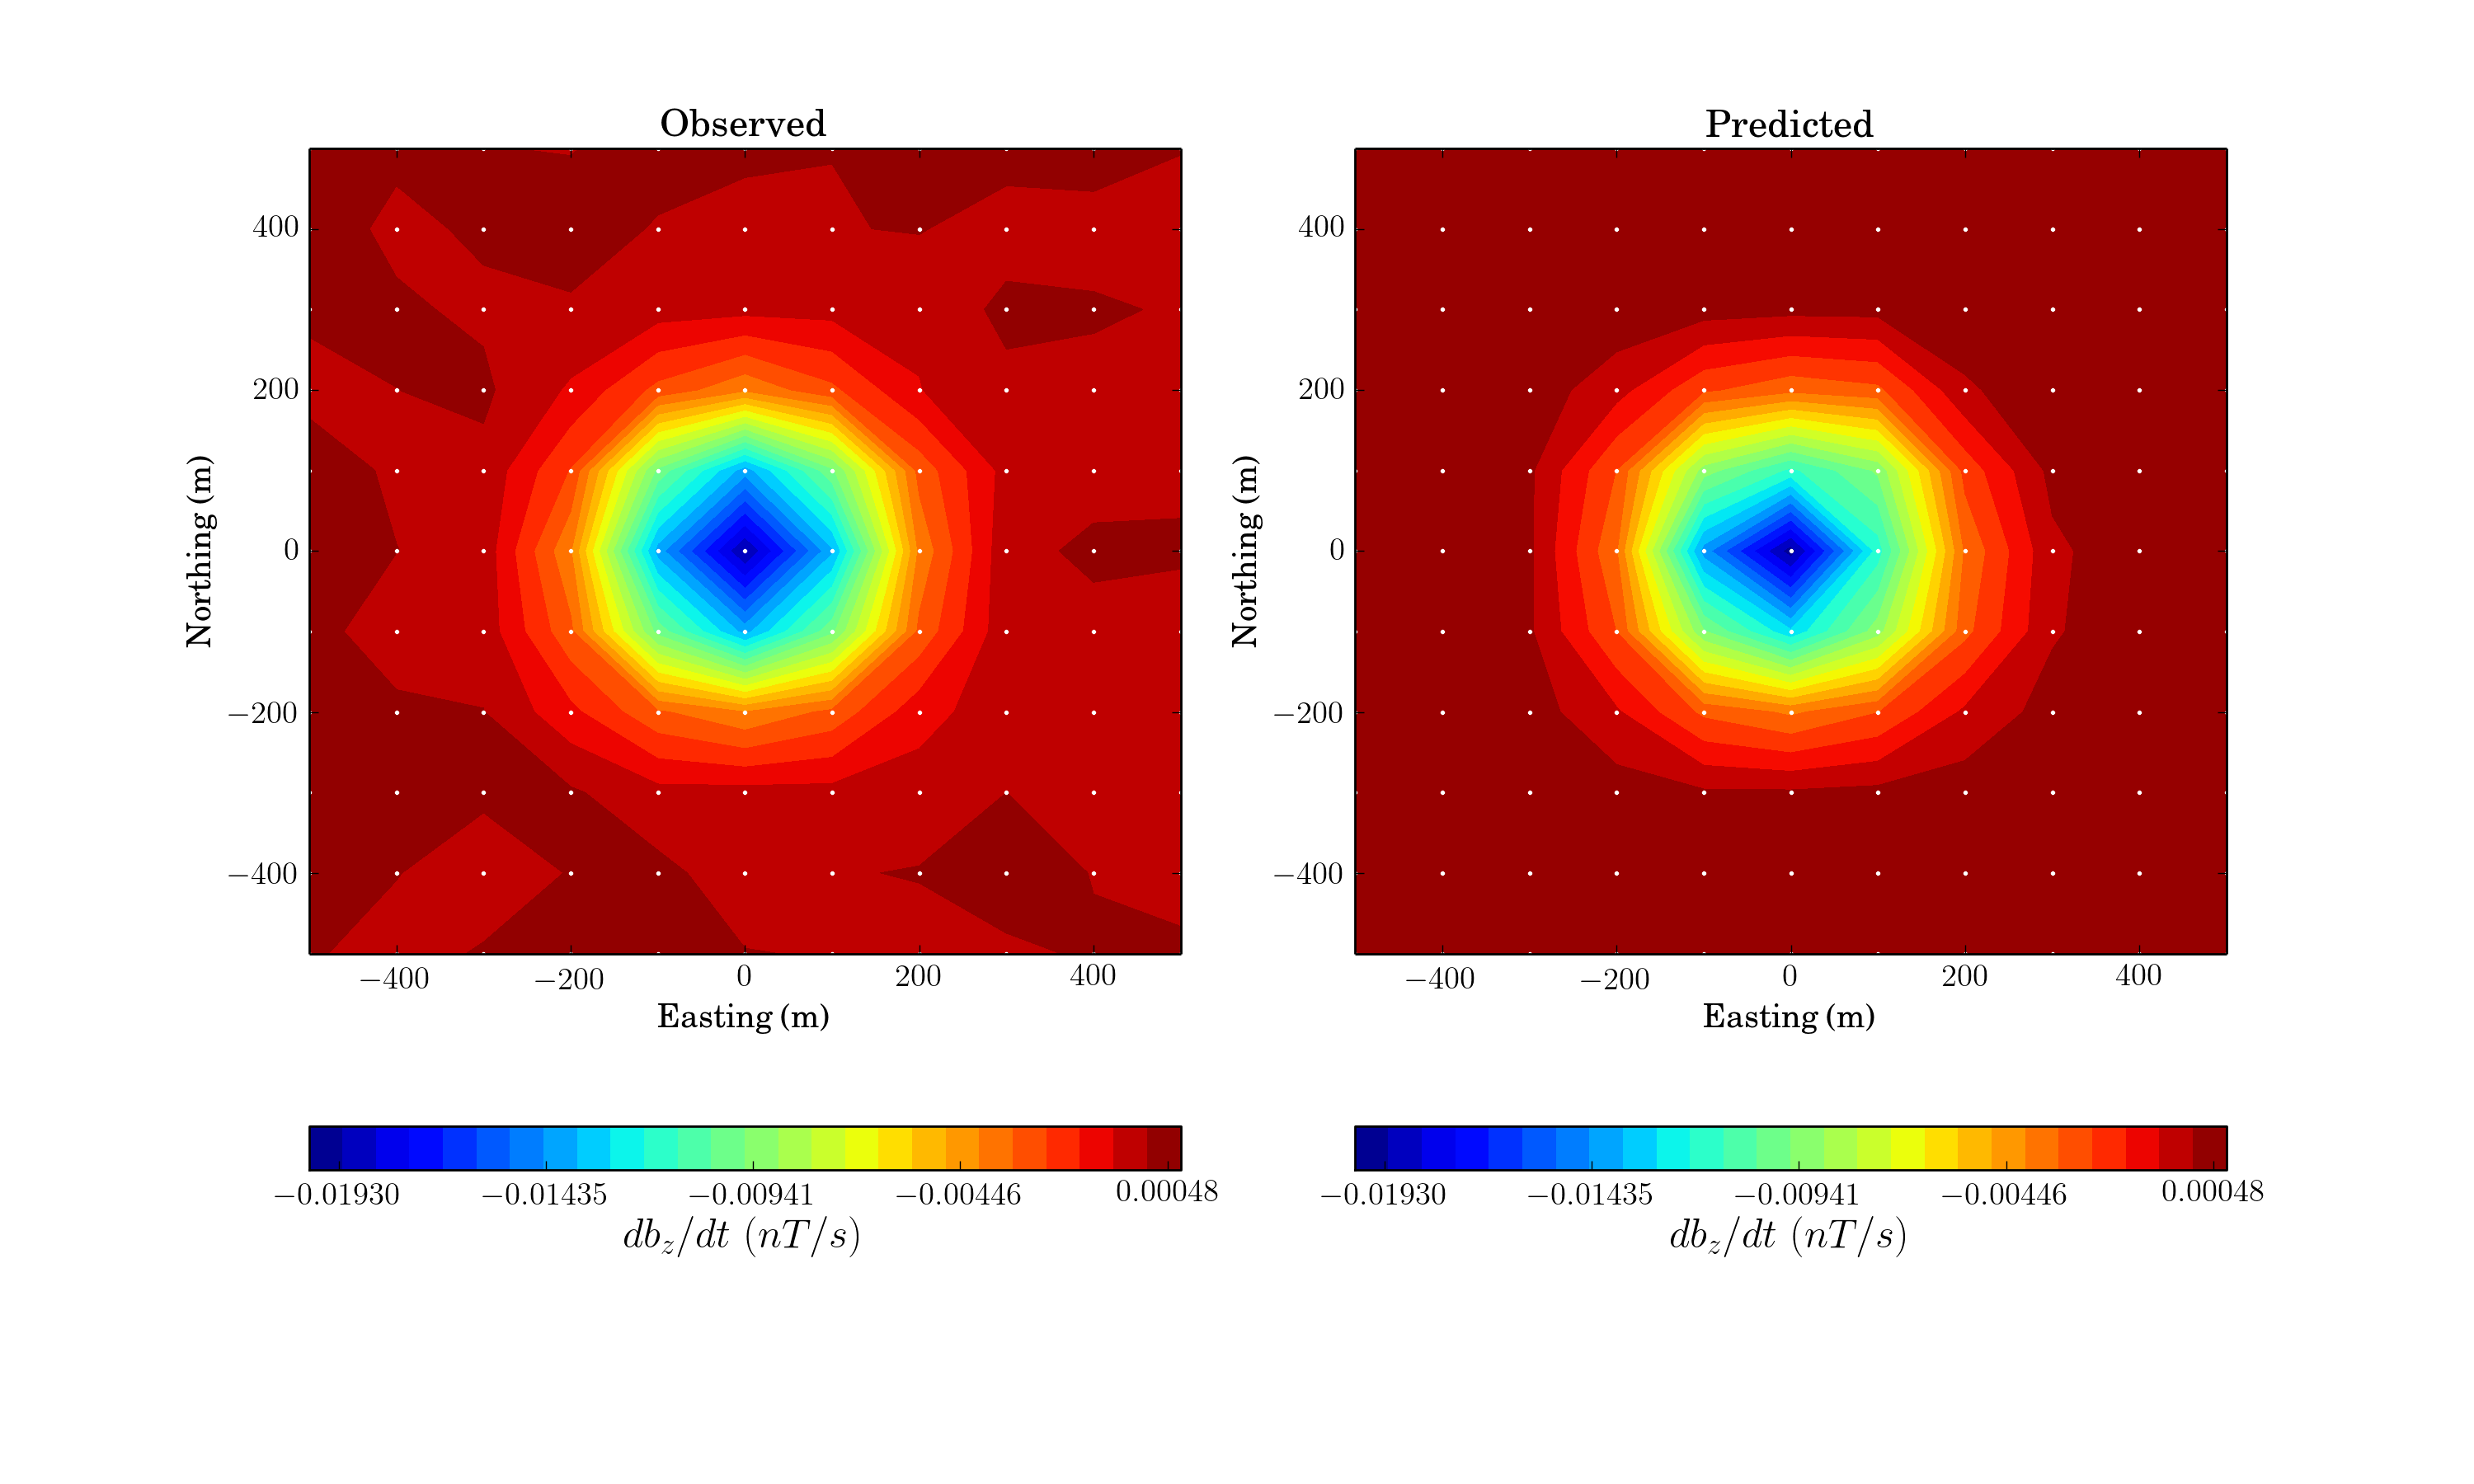
\includegraphics[width=\textwidth]{figures/synthetic/ObsPred_syn_ch38_case1.png}\\
%   (a)
%   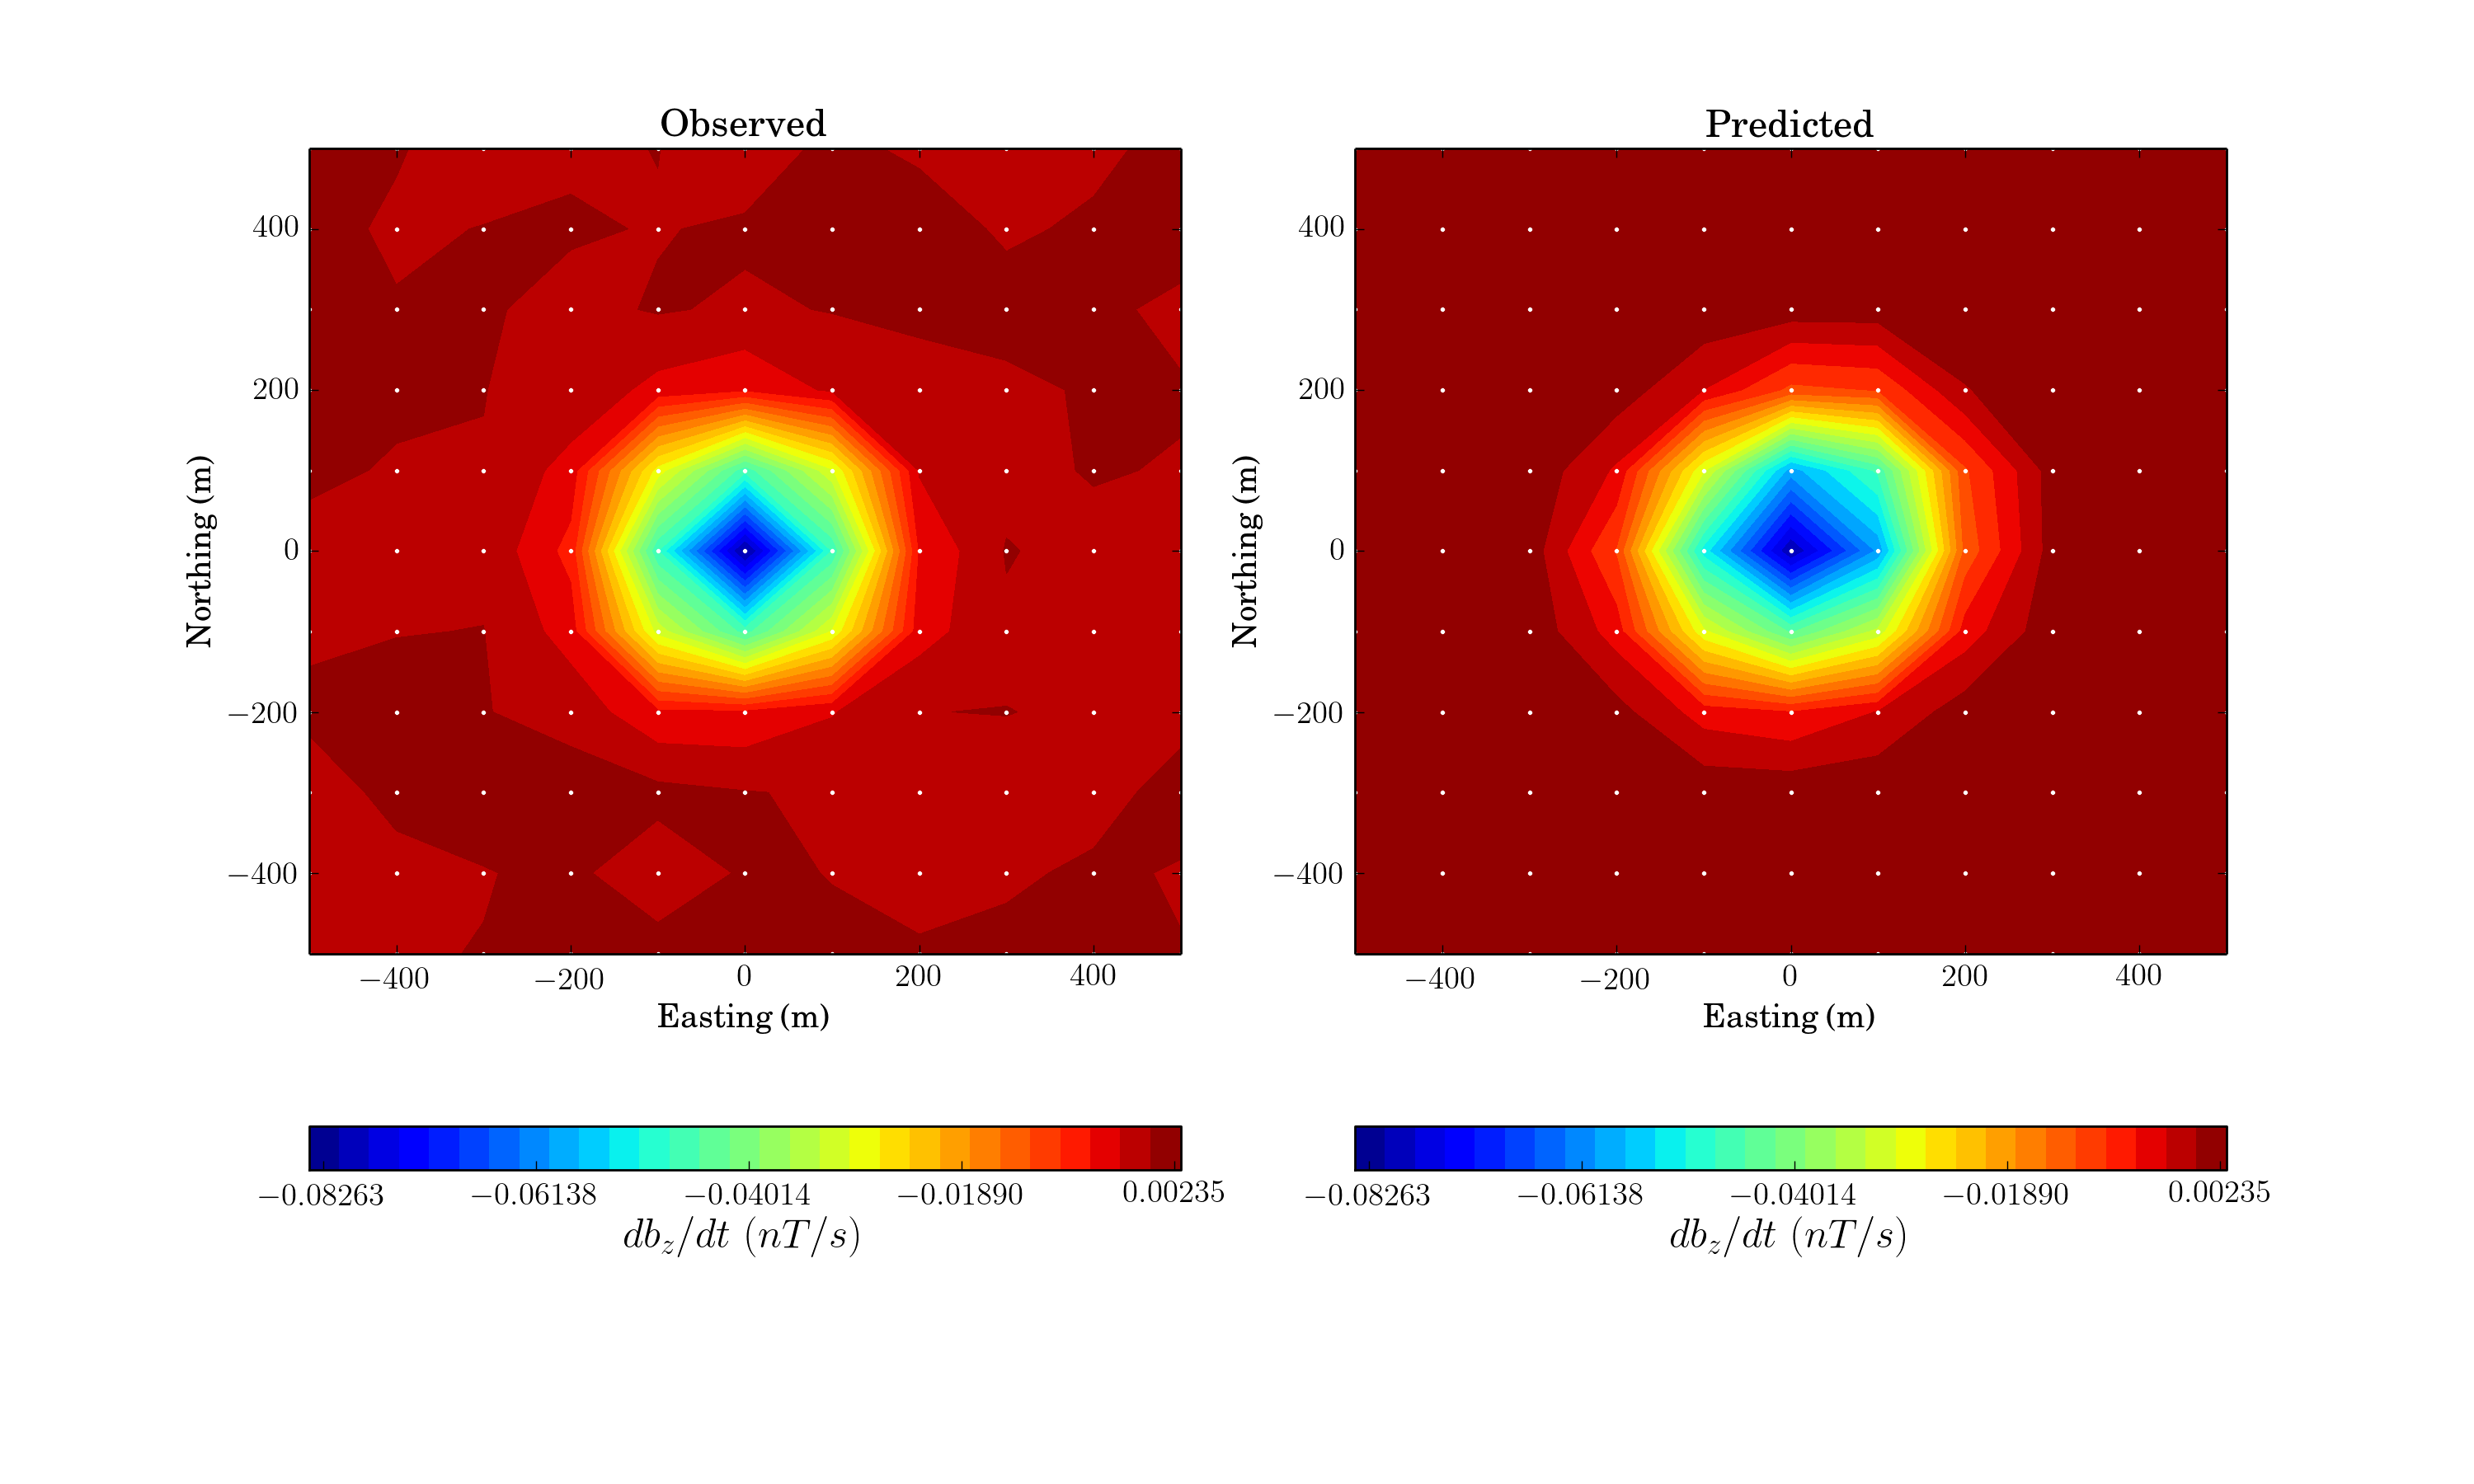
\includegraphics[width=\textwidth]{figures/synthetic/ObsPred_syn_ch38_case2.png}\\
%   (b)
%   \caption{Slices of estimated $\peta$ distributions at $t = $ 4.7 ms by inverting $\dip_{syn}$. (a) Canonical model. (b)  Conductive model. Left and right panel show plan and section view at -125 m depth and 0 m northing. Black dashed lines outline IP body. }
%   \label{F: ObsPred_syn_ch38}
% \end{figure}

% On the other hand, we consider true $\dip$ data at t=4.7 ms, which was generated by subtracting $d^{F}$ from $d$ as shown in the right panels of Figures ~\ref{F: EMIPresp2_case1}b and ~\ref{F: EMIPresp2_case2}b. Since $\peta$ is convoluted property of electric field and $\peta^{I}$, we need to evaluate restored $\peta$ can suggest meaningful information about the embedded IP body. Same survey configuration and inversion parameters were used as above examples for $\dip_{syn}$ except $r_{\beta}$=0.1. In Figure ~\ref{F: Peta_dip_ch38}a and b, we presented restored pseudo-chargeability models for both canonical and conductive models, respectively. Both inversions for canonical and conductive models were reached to the target misfit. Recovered $\peta$ models for both cases show reasonable geometry of IP body, whereas absolute magnitude of them are quite different from $\peta^{I}$. However, $\peta$ is convoluted property of $\e(t)$ and $\peta^{I}$ so that absolute value of restored $\peta$ does not have meaningful information. Therefore, restored $\peta$ can suggest geometry of IP body in the earth. Similar patterns from recovered $\peta$ models of $\dip_{syn}$ can be observed here: restored model from canonical model show broader distribution and smaller magnitude of $\peta$ than that from conductive model. Accordingly, identification of relative strength of $\peta^I$ for different IP bodies might depend on background conductivity model. In addition, to investigate effect of wrong background model, we invert $\dip$ data for conductive model using sensitivity matrix generated for canonical model. Restored $\peta$ distribution is shown in Figure ~\ref{F: Peta_case2_wrong_ch38} and it is almost same as Figure ~\ref{F: Peta_dip_ch38}b, which used correct sensitivity matrix. This shows the robustness of our inversion to background conductivity model. However, note that this effect in EM decoupling process can be more significant.

% \begin{figure}[htb]
%   \centering
%   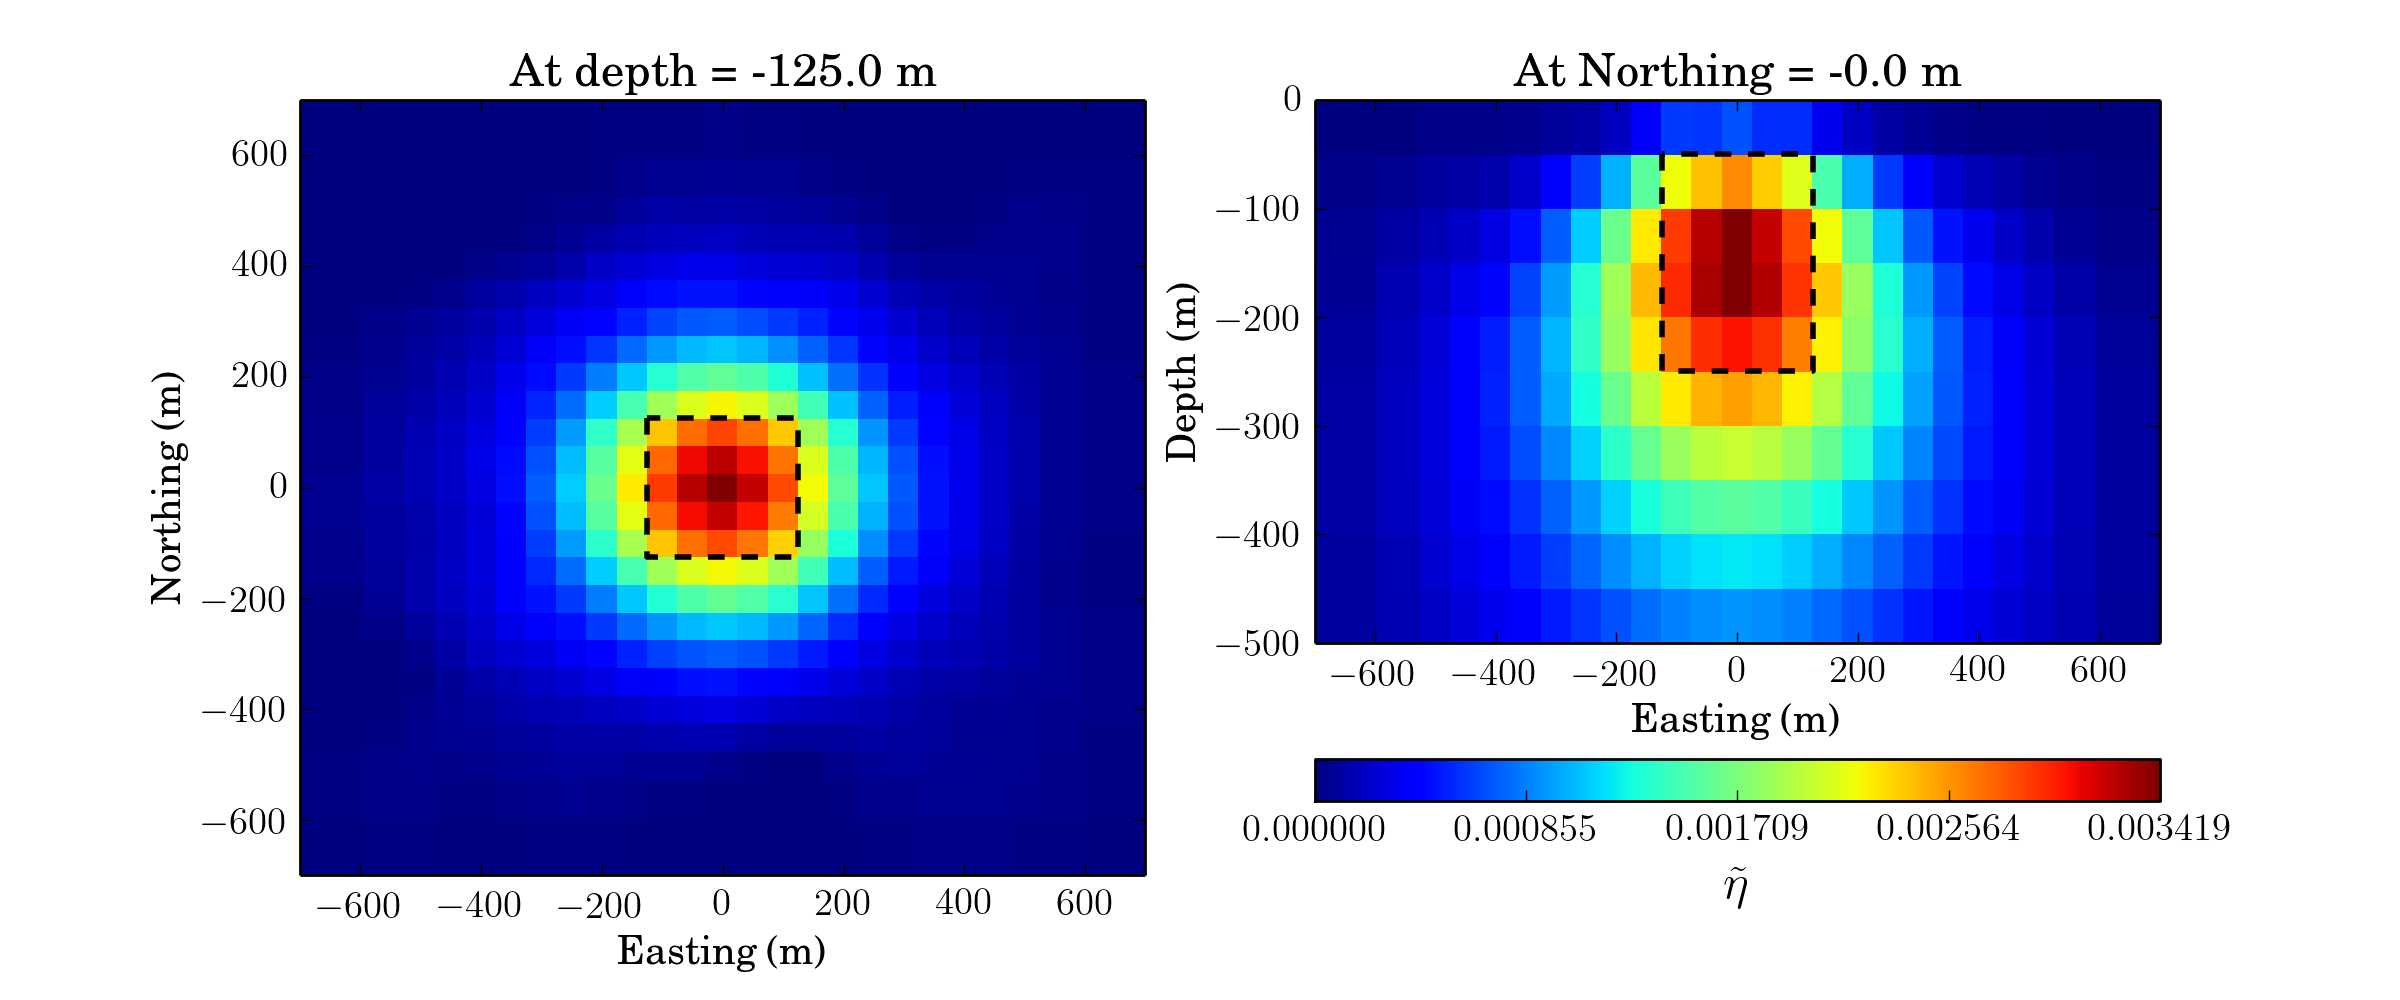
\includegraphics[width=\textwidth]{figures/synthetic/PetaCase1_true_ch38.png}\\
%   (a)
%   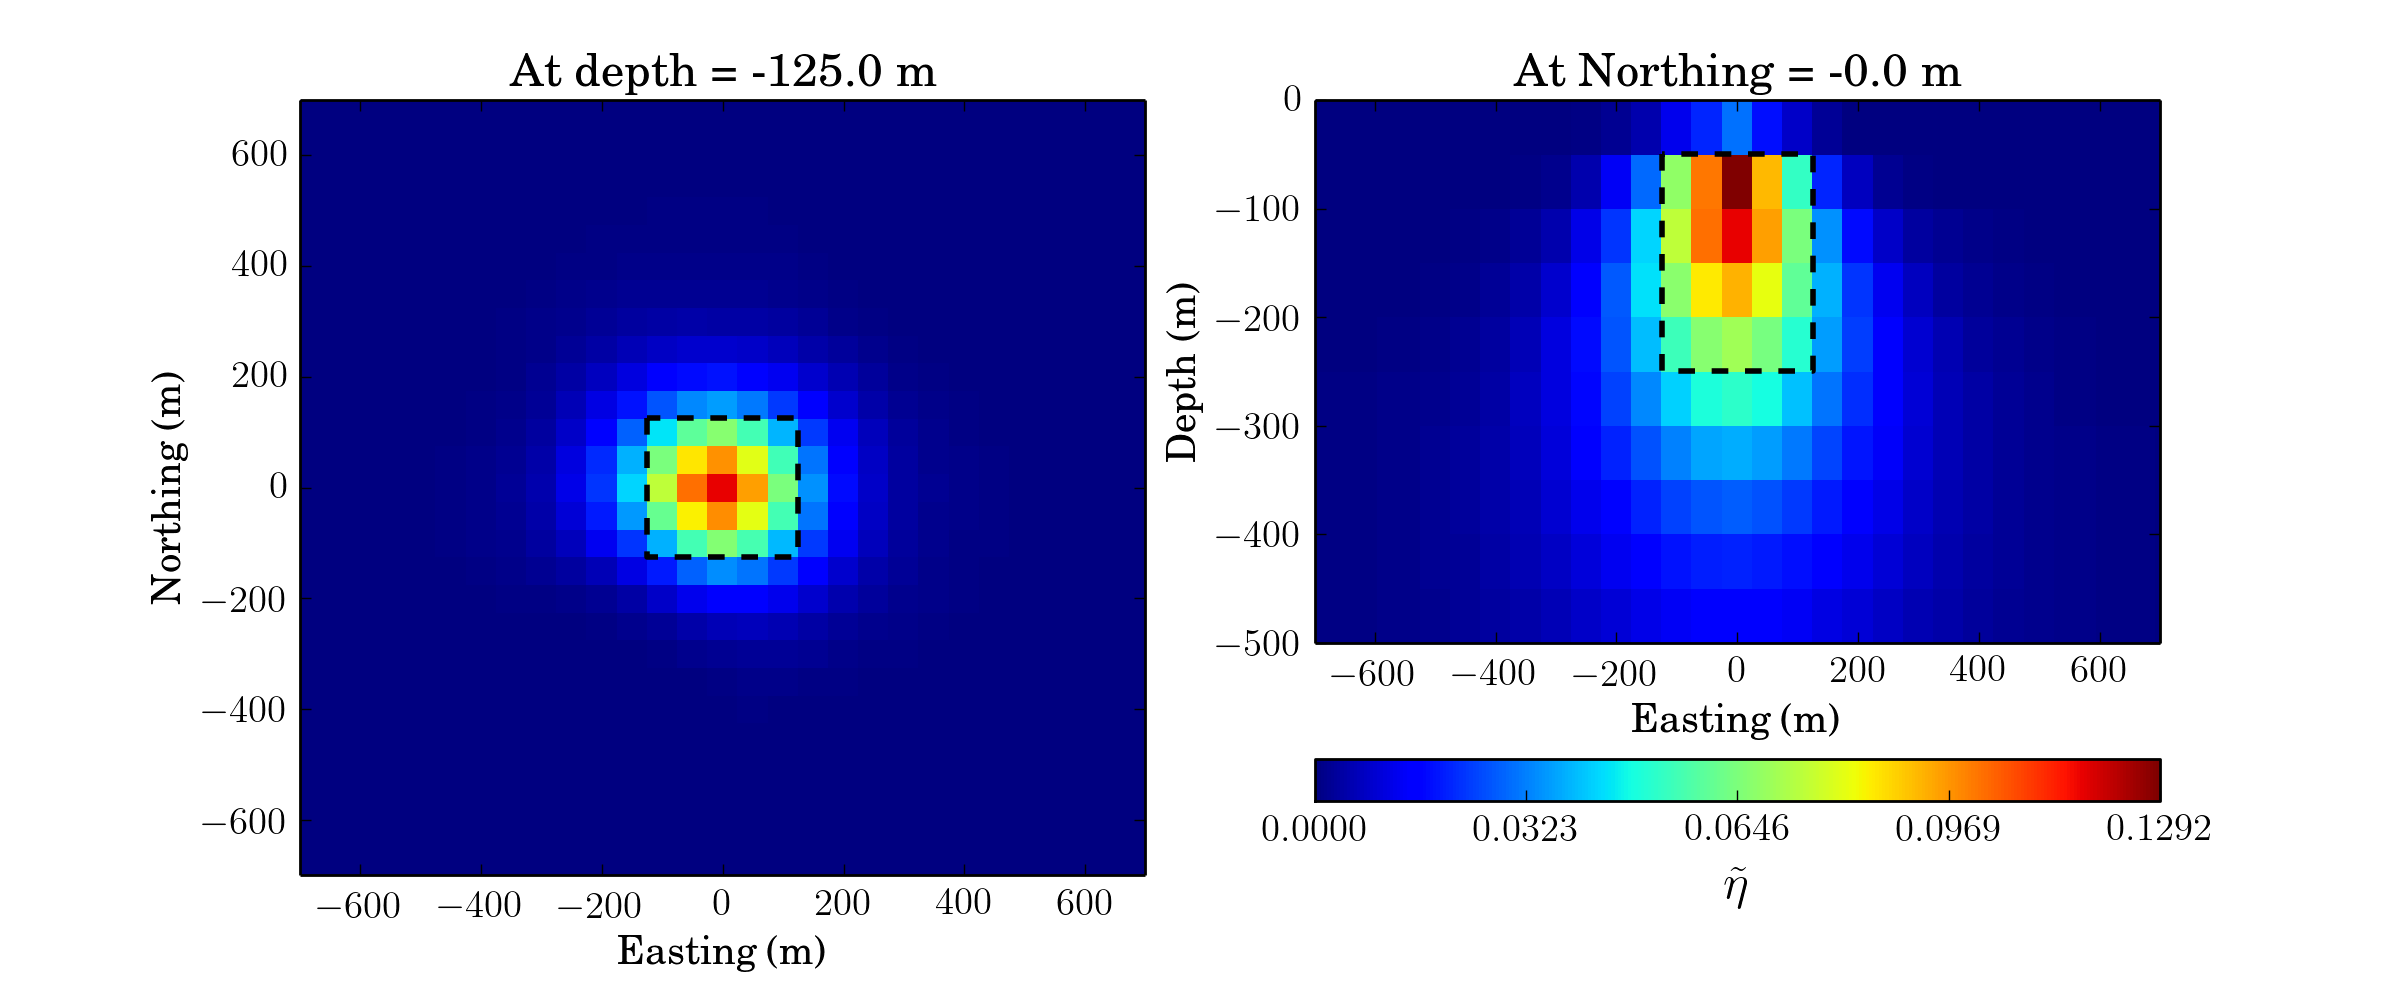
\includegraphics[width=\textwidth]{figures/synthetic/PetaCase2_true_ch38.png}\\
%   (b)
%   \caption{Slices of estimated $\peta$ distributions at $t = $ 4.7 ms  by inverting $\dip$. (a) Canonical model. (b)  Conductive model.. Left and right panel show plan and section view at -125 m depth and 0 m northing. }
%   \label{F: Peta_dip_ch38}
% \end{figure}

% \begin{figure}[htb]
%   \centering
%   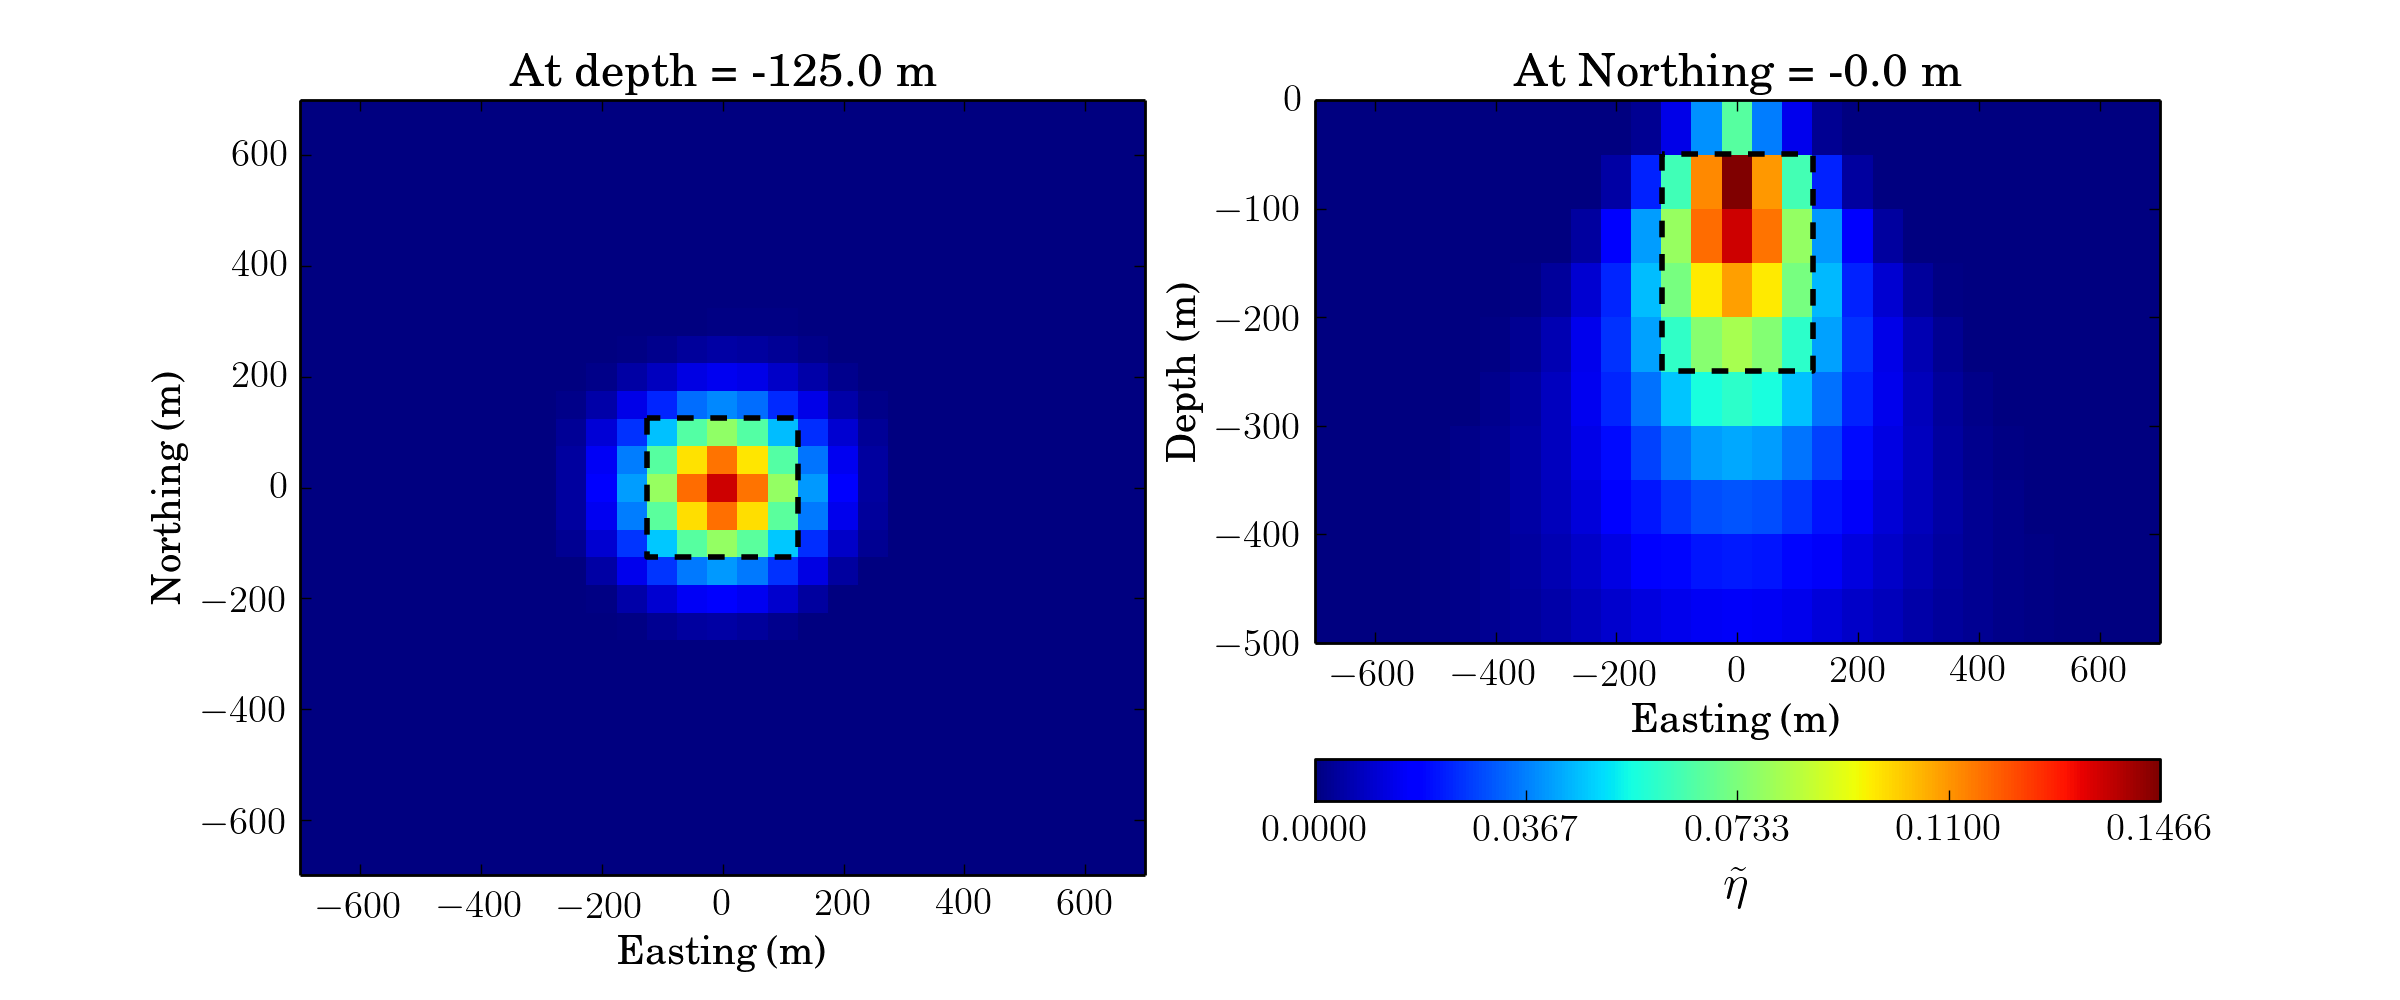
\includegraphics[width=\textwidth]{figures/synthetic/PetaCase2_wrong_ch38.png}
%   \caption{Slices of estimated $\peta$ distributions at $t = $ 4.7 ms for conductive model with incorrect background conductivity model. Left and right panel show plan and section view at -125 m depth and 0 m northing. }
%   \label{F: Peta_case2_wrong_ch38}
% \end{figure}

% Finally, using same survey and inversion set-ups, we inverted 14 time channels of $\\dip$ ranging from 1 to 10 ms for both cases. We presented time decaying curves of restored $\peta$ models at (0, 0, -125) for both cases in Figure ~\ref{F: Peta_Center}a and b. Since we already recognized absolute value of the estimated pseudo-chargeability, $\peta_{est}$ is not meaningful, significant magnitude difference between $\peta^{est}$ and $\peta^I$ makes sense. However, we identify slope of $\peta^{est}$ and $\peta^I$ looks similar in later time channels (2-10 ms) for both cases. Taking log to equation (\ref{eq: intrinsic_peta}) yields
% \begin{equation}
%     log(\peta^{I}) = log(\frac{\eta}{(1-\eta)\tau}) - \frac{1}{(1-\eta)\tau}t,
% \end{equation}
% which can be considered as linear equation. To estimate slope of the above equation, $- \frac{1}{(1-\eta)\tau}$, we fit active set of the recovered pseudo chageability, $\peta^{est}_{active}$ ranging from 2.5 ms to 10 ms. Estimated slopes for canonical and conductive models are -203 and -218 when the true slope is -250. Corresponding relative errors are 12 and 13$\%$. This is promising result, which suggests potential of restoring intrinsic Cole-Cole parameters from recovered $\peta$ model at each time channel.

% \begin{figure}[htb]
%   \centering
%   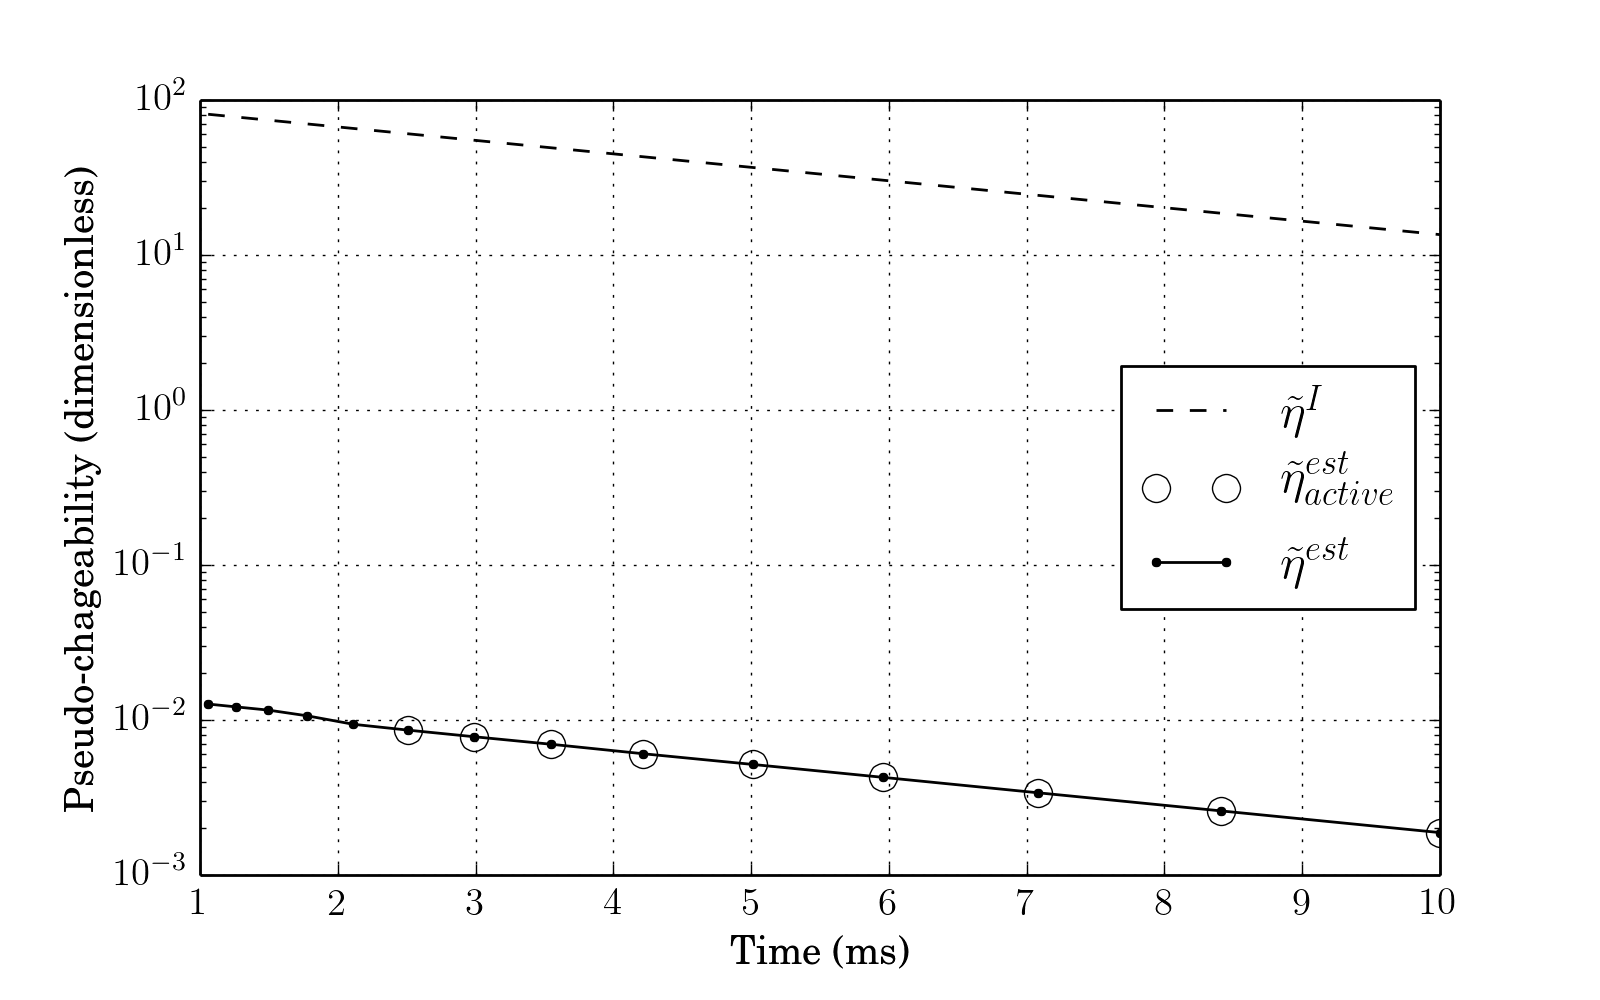
\includegraphics[width=0.8\textwidth]{figures/synthetic/PetaCase1_center.png} \\(a)\\
%   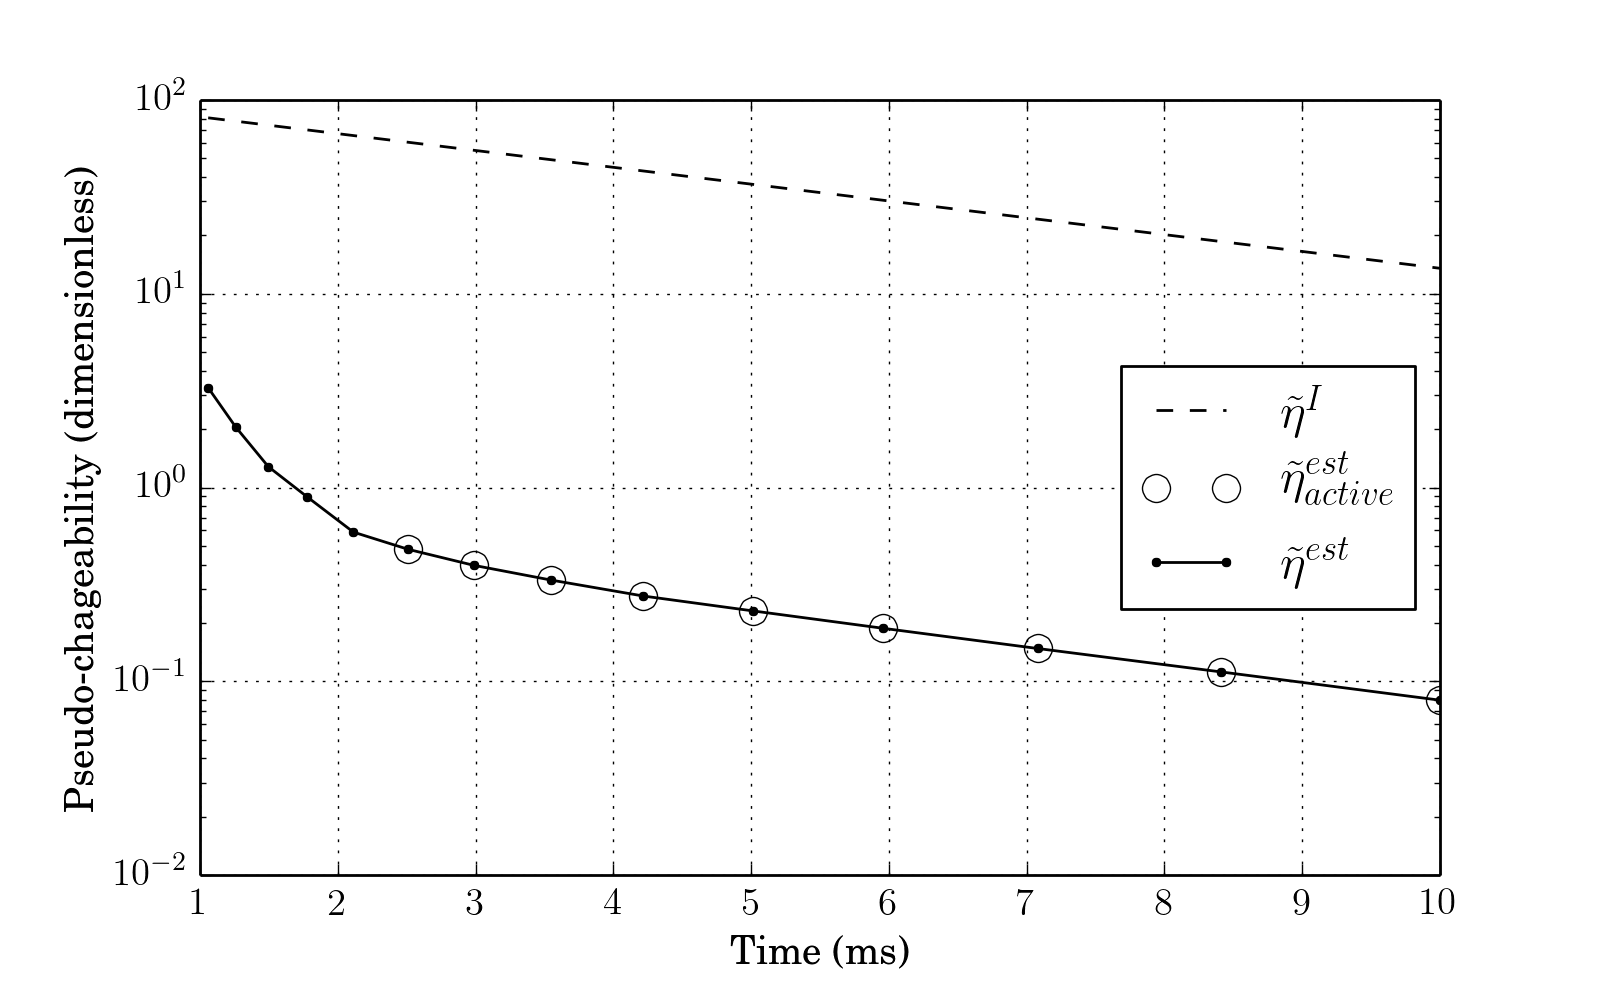
\includegraphics[width=0.8\textwidth]{figures/synthetic/PetaCase2_center.png} \\(b)
%   \caption{Time decaying curves of recovered and intrinsic pseudo chargeability at (0, 0, -125). (a) Canonical model. (b) Conductive model. Black dashed and solid line with solid circle indicate $\peta^{I}$ and $\peta^{est}$. Empty circles indicate active set of $\peta^{est}$, which are used to compute slope of time decaying $\peta^{est}$ in semi-log plot. }
%   \label{F: Peta_Center}
% \end{figure}

% \clearpage
% \subsection{Field example: Mt. Milligan}
% % \subsection{EIP}
% % \subsection{MIP}
% % \subsection{EM-IP with grounded source}
% % \subsection{EM-IP with inductive source (ATEM) }

% \clearpage

%% =======================================================================
%% SECTION (Appendix)
%% =======================================================================

% \section{Appendix}
% \subsection{Derivation of the sensitivity   in discretized space}
% The numerical evaluation of Maxwell's equations for the steady-state case can be derived by discretizing the system in space using finite volume (FV) method with weak formulation (CITE). For the discretization, we assume that the electric field $\e$ is discretized by grid function $\de$ on cell edges and magnetic flux density $\b$ is discretized by grid fuction $\db$ on cell faces. Electrical potential $\phi$ is discretized by grid fucntion  $\phi$ on cell nodes. For clear representation of the derivation, recall Maxwell's equations in steady state as
% \begin{align}
%   \j = \sigma\e = -\sigma\grad \phi, \\
%   -\div \j = \div \j_s, \\
%   \j\big|_{\partial \Omega}\cdot\hat{n} = 0,
%   \label{eq:DCBCneumann}
% \end{align}
% where $\partial \Omega$ indicates boundary surface of the system and $\hat{n}$ is the normal vector of the boundary surface. Modified from CITE, weak form of those equations can be written as
% \begin{align}
%   (\j, \vec{w}) + (\sigma \grad \phi, \vec{w}) = 0, \\
%   -(\j, \grad \psi) = (\j_s, \grad \psi).
% \end{align}
% The inner products $(\j, \vec{w})$, $(\sigma \grad \phi, \vec{w})$,  $(\j, \grad \psi)$ and $(\j_s, \grad \psi)$ are edge based products. Here we define the inner product as
% \begin{equation}
%   (\vec{a}, \vec{b}) = \int_{\Omega} \vec{a}\cdot\vec{b} dv,
% \end{equation}
% where $\Omega$ is the volume of the system. By discretizing $\grad$ operator and the inner product in space, we obtain
% \begin{equation}
%   \Me\dj + \MeSig\dgrad\phi = 0,
%   \label{eq:DCdisceq1}
% \end{equation}
% \begin{equation}
%   -\dgrad^T \Me\dj = \dgrad^T \Me\dj_s,
%   \label{eq:DCdisceq2}
% \end{equation}
% where $\mathbf{M}^e_i$ is the mass matrices, which discretize the edge based inner product (CITE). This inner products are defined  as
% \begin{align}
%   \mathbf{M}^e_i = \diag(\Ace^T\diag(\vol)\mathbf{i}).
% \end{align}
% Here, $\mathbf{i}$ indicates a grid function on cell center like $\sigma$, and $\vol$ is the grid function for the cell volume. The averaging matrix $\Ace$ averages discrete function defined on the edges to the cell center. The mass matrix $\Me$ without subscript $i$ indicates that $\mathbf{i}$ is equal to the identity column vector of which all elements are one. By substituting equation (\ref{eq:DCdisceq1}) to (\ref{eq:DCdisceq2}), we have
% \begin{equation}
%   \A^{DC}\phi = \mathbf{rhs}^{DC},
%   \label{eq:DCdiscLin}
% \end{equation}
% where $\A^{DC} = \dgrad^T \MeSig\dgrad$ and $\mathbf{rhs}^{DC} = \dgrad^T \Me\dj_s$. Sensitivity function of $\phi$ can be derived by taking derivative to equation (\ref{eq:DCdiscLin}) in terms of $\sigma$:
% \begin{equation}
%   \frac{\partial \phi}{\partial \sigma} = -(\A^{DC})^{-1}\dgrad^T\diag(\dgrad\phi)\Ace^T\diag(\vol).
%   \label{eq:DCsensedisc}
% \end{equation}
% We recall that continuous sensitivity function shown in equation (\ref{eq: senseDC}), which can be modified as
% \begin{equation}
%   \frac{\partial \phi}{\partial \sigma} = -[\div\sigma\grad]^{-1}\div\grad\phi.
%   \label{eq:DCsensecont}
% \end{equation}
% One can intuitively identify that continuous sensitivity function shown in equation (\ref{eq:DCsensecont}) can be discretized as equation (\ref{eq:DCsensedisc}) with the boundary condition specified on equation (\ref{eq:DCBCneumann}). This approach shows that some advantages of working in discretized space even for the derivation of continuous function (CITE).

% \subsection{Discretization of linear IP problem}
% In order to restore distributed $\peta(x, y, z; t)$ in 4D space, first we need to discretize Biot-Savart law shown in equations (\ref{eq: BiotbIP_approx}) and (\ref{eq: BiotbIPdt_approx}). In addition, based on the discretization that we choose, we need to compute $\e^{F}_{max}$. In our discretization $\j^{IP}$ and  $\tilde{\eta}_w$ are defined on the cell center, and those for each time channel are constant in a cell volume, whereas $\e^{F}_{max}$ is defined on the cell edges. We define the number of cells and edges in 3D space as nC and nE, respectively. Assuming we have discretized IP current densitivity distribution ($\dj^{IP}_{cc}$), which has dimension: [(3nC)$\times$1] and defined on the cell center, since $\j^{IP}$ has three components, we first discretize integration operator including cross product ($\int_{v}\frac{ \times \hat{r}}{r^2}dv$) as
% \begin{equation}
%   \mathbf{G}_{Biot} =
%   \begin{bmatrix}
%        \mathbf{e}^T &  \mathbf{0}   & \mathbf{0}  \\
%        \mathbf{0}   &  \mathbf{e}^T & \mathbf{0}  \\
%        \mathbf{0}   &  \mathbf{0}   & \mathbf{e}^T
%     \end{bmatrix}
%   \begin{bmatrix}
%        \mathbf{0}     &   \mathbf{S}_z   & -\mathbf{S}_y  \\
%       -\mathbf{S}_z   &   \mathbf{0}     &  \mathbf{S}_x  \\
%        \mathbf{S}_y   &  -\mathbf{S}_x   &  \mathbf{0}
%     \end{bmatrix},
%  \end{equation}
% where
% \begin{eqnarray*}
%   \mathbf{S}_i =\diag(\mathbf{r}_i \oplus \frac{1}{\mathbf{r}^2}), \ i = x, \ y, \ z
% \end{eqnarray*}
% and $\mathbf{e}$ is a column vector of which element is 1 and has the dimension: [nC$\times$1], $\diag(\cdot)$ is the diagonal matrix and $\oplus$ is the Hadamard product. Then we consider discrete expression for $\j^{IP}$ shown in equation (\ref{eq: jip_approx}), and modify this equation as
% \begin{eqnarray}
%   \dj^{IP}_{cc}(t) = -\mathbf{S}\diag(\de^{F}_{max})\Ace^T\diag(\vol)\diag(\siginf)\peta(t),
% \end{eqnarray}
% where
% \begin{eqnarray}
%   \mathbf{S} = \mathbf{A}^{e}_{ccv}\Me^{-1}[-\MeSigInf \mathbf{G} \A_{\siginf}^{-1}\mathbf{G}^T + \mathbf{I}] \diag(\de^{F}_{max})\Ace^T\diag(\vol)\diag(\siginf).
% \end{eqnarray}
% and $\mathbf{A}^{e}_{ccv}$ is discrete averaging matrix from edge to cell center with consideration of three component vector so that dimension of this matrix is [3nC$\times$nE]. Thus, we can have linear equation for $k^{th}$ time channel as
% \begin{eqnarray*}
%   \db^{IP}_k = -\Gbiot \mathbf{S} \peta_k,
% \end{eqnarray*}
% where sub-index $k$ indcates $k^{th}$ time channel. Finally, by letting
% \begin{equation}
%   \mathbf{J} = -\Gbiot\mathbf{S},
%   \label{eq: Sense}
% \end{equation}
% we have
% \begin{eqnarray}
%   \db^{IP}_k = -\mathbf{J}\peta_k,
%   \label{eq: bIP_linear}
% \end{eqnarray}
% where $\mathbf{J}$ is the Jacobian matrix of the linear equation, and since $\mathbf{J}$ is not time-dependent we also have
% \begin{eqnarray}
%   \frac{\partial\db^{IP}_k}{\partial t} = -\mathbf{J}\frac{\partial}{\partial t}\peta_k.
%   \label{eq: dbIPdt_linear}
% \end{eqnarray}
% Therefore, we can restore distributed $\peta(t)$ or $\frac{\partial}{\partial t}\peta(t)$ based on the data type we have. Note that problems shown in equations (\ref{eq: bIP_linear}) and (\ref{eq: dbIPdt_linear}) are linear problems; thus, by solving linear inverse problem for each time channel we can recover distributed IP parameters. Detailed description about discrete operators are shown in Appendix ??.

\clearpage
\bibliographystyle{plain}
\bibliography{reference}

\end{document}



% http://www.math.mun.ca/tex-archive/macros/latex/contrib/todonotes/todonotes.pdf
